% !TEX TS-program = xelatex
% Command for running this example (needs latexmkrc file):
%    latexmk -bibtex -pdf main.tex

%	نمونه پایان‌نامه آماده شده با استفاده از کلاس tehran-thesis، نگارش 1
%	سینا ممکن، دانشگاه تهران 
%	https://github.com/sinamomken/tehran-thesis
%	گروه پارسی‌لاتک
%	http://www.parsilatex.com
%	این نسخه، بر اساس نسخه‌ 0.1 از کلاس IUST-Thesis آقای محمود امین‌طوسی آماده شده است.
%        http://profsite.sttu.ac.ir/mamintoosi

%----------------------------------------------------------------------------------------------
% اگر قصد نوشتن پروژه کارشناسی را دارید، در خط زیر به جای msc، کلمه bsc و اگر قصد نوشتن رساله دکترا را دارید، کلمه phd را قرار دهید. کلیه تنظیمات لازم، به طور خودکار، اعمال می‌شود.

% اگر مایلید پایان‌نامه شما دورو باشد به جای oneside در خط زیر از twoside استفاده کنید.

% برای حاشیه‌نویسی و کم کردن صفحات ابتدایی، گزینه draft را وارد و برای نسخه نهایی آن را حذف کنید.

% برای استفاده از قلم‌های سری IR Series گزینه irfonts را وارد و برای استفاده از قلم‌های X Series 2 آن را حذف کنید.
\ExplSyntaxOn
\cs_set_eq:NN
\etex_iffontchar:D
\tex_iffontchar:D
\cs_undefine:N \c_one
\int_const:Nn \c_one { 1 }
\ExplSyntaxOff

\documentclass[
twoside
% ,openany
,bsc
,irfonts
% ,draft
]{./tex/tehran-thesis}

\newcommand{\mc}[1]{\mathcal{#1}}



% فایل commands.tex را مطالعه کنید؛ چون دستورات مربوط به فراخوانی بسته‌ها، فونت و دستورات خاص در این فایل قرار دارد.
% در این فایل، دستورها و تنظیمات مورد نیاز، آورده شده است.
%-------------------------------------------------------------------------------------------------------------------
% دستوراتی که پوشه پیش‌فرض زیرفایل‌های tex را مشخص می‌کند.
%\makeatletter
%\def\input@path{{./tex/}}
%\makeatother
\usepackage{mathtools}
% در ورژن جدید زی‌پرشین برای تایپ متن‌های ریاضی، این سه بسته، حتماً باید فراخوانی شود
\usepackage{amsthm,amssymb,amsmath}
% بسته‌ای برای تنطیم حاشیه‌های بالا، پایین، چپ و راست صفحه
\usepackage[a4paper, top=40mm, bottom=40mm, outer=25mm, inner=35mm]{geometry}
% بسته‌‌ای برای ظاهر شدن شکل‌ها و تعیین آدرس تصاویر
\usepackage[final]{graphicx}
\usepackage{booktabs}
\graphicspath{{./img/}}
% بسته‌های مورد نیاز برای نوشتن کدها، رنگ‌آمیزی آنها و تعیین پوشهٔ کدها
\usepackage[final]{listings}
\usepackage[usenames,dvipsnames,svgnames,table]{xcolor}
\lstset{inputpath=./code/}
% بسته‌ای برای رسم کادر
\usepackage{framed} 
% بسته‌‌ای برای چاپ شدن خودکار تعداد صفحات در صفحه «معرفی پایان‌نامه»
\usepackage{lastpage}
% بسته‌ٔ لازم برای: ۱. تغییر شماره‌گذاری صفحات پیوست. ۲. تصحیح باگ آدرس وب حاوی '%' در مراجع
\usepackage{etoolbox}

%%%%%%%%%%%%%%%%%%%%%%%%%%%%%%%%%%%%
%%% دستورات وابسته به استیل مراجع:
%% اگر از استیل‌های natbib (plainnat-fa، asa-fa، chicago-fa) استفاده می‌کنید، خط زیر را فعال و بعدی‌اش را غیرفعال کنید.
%\usepackage{natbib}
%\newcommand{\citelatin}[1]{\cite{#1}\LTRfootnote{\citeauthor*{#1}}}
%\newcommand{\citeplatin}[1]{\citep{#1}\LTRfootnote{\citeauthor*{#1}}}
%% اگر از سایر استیل‌ها استفاده می‌کنید، خط بالا را غیرفعال و خط‌های زیر را فعال کنید.
\let\citep\cite
\let\citelatin\cite
\let\citeplatin\cite
%%%%%%%%%%%%
% بررسی حالت پیش نویس
\usepackage{ifdraft}
\ifdraft
{%
	% بسته‌ٔ ایجاد لینک‌های رنگی با امکان جهش
	\usepackage[unicode=true,pagebackref=true,
	colorlinks,linkcolor=blue,citecolor=blue,final]{hyperref}
	%\usepackage{todonotes}
	\usepackage[firstpage]{draftwatermark}
	\SetWatermarkText{\ \ \ پیش‌نویس}
	\SetWatermarkScale{1.2}
}
{ 
	\usepackage[pagebackref=false]{hyperref}
	%\usepackage[disable]{todonotes} % final without TODOs
}

\usepackage[obeyDraft]{todonotes}
\setlength{\marginparwidth}{2cm}

\usepackage{tikz}
\usepackage{tikzit}
\usepackage{pgfplots}
%\usepackage{subcaption}
% \usepackage{hyperref}

\usepackage{anyfontsize}
% TiKZ style file generated by TikZiT. You may edit this file manually,
% but some things (e.g. comments) may be overwritten. To be readable in
% TikZiT, the only non-comment lines must be of the form:
% \tikzstyle{NAME}=[PROPERTY LIST]

% Node styles
\tikzstyle{node}=[fill={rgb,255: red,165; green,162; blue,255}, draw={rgb,255: red,51; green,42; blue,179}, shape=circle, minimum size=10]
\tikzstyle{empty_node}=[draw={rgb,255: red,51; green,42; blue,179}, shape=circle]
\tikzstyle{Rec}=[draw=black, shape=rectangle, minimum width=3cm, minimum height=3.5cm]
\tikzstyle{X_wrapper}=[draw=black, shape=rectangle, minimum width=3cm, minimum height=3cm]
\tikzstyle{red_node}=[fill={rgb,255: red,255; green,185; blue,186}, draw={rgb,255: red,143; green,21; blue,38}, shape=circle]
\tikzstyle{layer_1_wrapper}=[draw=black, shape=rectangle, minimum width=4cm, minimum height=16.5cm, line width=3pt, rounded corners=0.4cm]
\tikzstyle{second_laeyr_wrapper}=[draw={rgb,255: red,51; green,11; blue,121}, shape=rectangle, minimum width=4cm, minimum height=28cm, fill={rgb,255: red,158; green,160; blue,255}, opacity=0.2, rounded corners=0.4cm]
\tikzstyle{EncoderWrapper}=[draw=black, shape=rectangle, minimum width=42cm, line width=5pt, minimum height=36cm, rounded corners=0.4cm]
\tikzstyle{description}=[inner sep=0mm, font={\fontsize{55}{50}\selectfont}]
\tikzstyle{description_layers}=[inner sep=0mm, font={\fontsize{45}{43}\selectfont}]
\tikzstyle{InputsWrapper}=[draw=black, shape=rectangle, minimum width=6.5cm, minimum height=8.5cm, rounded corners=0.2cm, line width=5pt]
\tikzstyle{MiniInputsWrapper}=[draw=black, shape=rectangle, minimum width=7cm, minimum height=8.5cm, rounded corners=0.2cm, line width=5pt]
\tikzstyle{Zprim}=[draw=black, shape=rectangle, minimum width=8.5cm, minimum height=6cm, rounded corners=0.2cm, line width=5pt]
\tikzstyle{Pz}=[draw=black, shape=rectangle, minimum width=8.5cm, minimum height=9cm, rounded corners=0.2cm, line width=5pt]
\tikzstyle{little_node}=[fill={rgb,255: red,165; green,162; blue,255}, draw={rgb,255: red,51; green,42; blue,179}, shape=circle, minimum size=0.01cm]
\tikzstyle{OutputsWrapper}=[draw=black, shape=rectangle, minimum width=4.5cm, minimum height=7cm, rounded corners=0.2cm, line width=5pt]
\tikzstyle{DecoderWrapper}=[draw=black, shape=rectangle, minimum width=10.5cm, minimum height=6cm, rounded corners=0.4cm, line width=5pt]
\tikzstyle{neuron}=[fill={rgb,255: red,60; green,53; blue,155}, draw={rgb,255: red,51; green,42; blue,179}, shape=circle, minimum size=0.6cm]
\tikzstyle{dense_1_layer}=[draw=black, shape=rectangle, minimum width=2cm, minimum height=5.7cm, rounded corners=0.04cm, line width=3pt]
\tikzstyle{dense_2_layer}=[draw=black, shape=rectangle, minimum width=2cm, minimum height=10cm, rounded corners=0.04cm, line width=3pt]
\tikzstyle{dense_x_layer}=[draw=black, shape=rectangle, minimum width=2cm, minimum height=3.7cm, rounded corners=0.04cm, line width=3pt]
\tikzstyle{Relu}=[draw=black, shape=rectangle, font={\fontsize{38}{43}\selectfont}]
\tikzstyle{discriminatorWrapper}=[draw=black, shape=rectangle, minimum width=35.5cm, minimum height=15cm, rounded corners=0.4cm, line width=5pt]
\tikzstyle{wraperDecoder}=[draw=black, shape=rectangle, minimum width=19cm, minimum height=15cm, rounded corners=0.4cm, line width=5pt]
\tikzstyle{discOuput}=[draw={rgb,255: red,67; green,29; blue,150}, shape=rectangle, minimum width=1cm, minimum height=1cm, rounded corners=0.04cm, fill={rgb,255: red,145; green,137; blue,255}, opacity=0.1]
\tikzstyle{discInput}=[draw=black, shape=rectangle, minimum width=5cm, minimum height=2.2cm, rounded corners=0.04cm, line width=5pt]
\tikzstyle{kmeans}=[draw=black, line width=5pt, shape=rectangle, minimum width=15.5cm, minimum height=3cm, rounded corners=0.04cm]
\tikzstyle{green_node}=[fill={rgb,255: red,32; green,92; blue,39}, draw={rgb,255: red,41; green,130; blue,44}, shape=circle]
\tikzstyle{yellow_node}=[fill={rgb,255: red,255; green,255; blue,69}, draw={rgb,255: red,217; green,220; blue,27}, shape=circle]
\tikzstyle{brown_node}=[fill={rgb,255: red,138; green,92; blue,46}, draw={rgb,255: red,158; green,105; blue,52}, shape=circle]
\tikzstyle{purple_node}=[fill={rgb,255: red,81; green,0; blue,81}, draw={rgb,255: red,98; green,0; blue,98}, shape=circle]
% V2
\tikzstyle{AXWrapper}=[draw=black, shape=rectangle, minimum width=6cm, minimum height=4.5cm, rounded corners=0.2cm, line width=5pt]
\tikzstyle{EnoderTitle}=[draw=black, shape=rectangle, minimum width=6.8cm, minimum height=4.5cm, rounded corners=0.2cm, line width=5pt]
\tikzstyle{ZZprim}=[draw=black, shape=rectangle, minimum width=8.6cm, minimum height=4.5cm, rounded corners=0.2cm, line width=5pt]
\tikzstyle{SingleWrapper}=[draw=black, shape=rectangle, minimum width=3cm, minimum height=3cm, rounded corners=0.2cm, line width=5pt]
\tikzstyle{GNN}=[draw=black, shape=rectangle, minimum width=8cm, minimum height=4cm, rounded corners=0.2cm, line width=5pt]
\tikzstyle{EncWrapper}=[draw=black, shape=rectangle, minimum width=46cm, line width=5pt, minimum height=24cm, rounded corners=0.4cm]
\tikzstyle{Little}=[font={\fontsize{38}{43}\selectfont}]
\tikzstyle{AdX}=[draw=black, shape=rectangle, minimum width=13cm, minimum height=5.5cm, rounded corners=0.2cm, line width=5pt]
\tikzstyle{Z}=[draw=black, shape=rectangle, minimum width=11cm, minimum height=3.5cm, rounded corners=0.2cm, line width=5pt]
\tikzstyle{EnccWrapper}=[draw=black, shape=rectangle, minimum width=32cm, line width=5pt, minimum height=30cm, rounded corners=0.4cm]
\tikzstyle{gnnLayer}=[draw=black, shape=rectangle, minimum width=4cm, minimum height=13cm, line width=3pt, rounded corners=0.4cm]
% Edge styles
\tikzstyle{new edge style 0}=[-, draw={rgb,255: red,72; green,36; blue,191}]
\tikzstyle{arrow}=[->, line width=4pt]

\newcommand{\revenueFig}[1]
{
\begin{tikzpicture}
  \begin{axis}
    [    
    bar width=20pt,
    ybar=0pt,
    enlargelimits=0.05,
    ylabel={Revenue},
    ylabel style={text height=0.02\textwidth,inner ysep=0pt},
    enlarge x limits=0.15,
    tickpos=left,
    scaled y ticks=base 10:-5,
    symbolic x coords={GRC, GraphViNE, Best Fit, First Fit, NeuroViNE},
    xtick=data,
    x tick label style={rotate=45,anchor=east},
    ]
    \addplot table[x=Name, y=Value, col sep=comma]{plots/revenues/data/#1.csv};
    
  \end{axis}
\end{tikzpicture}
}
\newcommand{\costFig}[1]
{
\begin{tikzpicture}
  \begin{axis}
    [    
    bar width=20pt,
    ybar=0pt,
    enlargelimits=0.05,
    ylabel={Cost},
    ylabel style={text height=0.02\textwidth,inner ysep=0pt},
    enlarge x limits=0.15,
    tickpos=left,
    scaled y ticks=base 10:-5,
    symbolic x coords={GRC, GraphViNE, Best Fit, First Fit, NeuroViNE},
    xtick=data,
    x tick label style={rotate=45,anchor=east},
    ]
    \addplot table[x=Name, y=Value, col sep=comma]{plots/costs/data/#1.csv};
    
  \end{axis}
\end{tikzpicture}
}

%%%%%%%%%%%%
%%% تصحیح باگ: اگر در مراجع، آدرس وب حاوی '%' بوده و pagebackref فعال باشد، دستورات زیر باید بیایند:
%% برای استیل‌های natbib مثل plainnat-fa، asa-fa، chicago-fa
\makeatletter
\let\ORIG@BR@@lbibitem\BR@@lbibitem
\apptocmd\ORIG@BR@@lbibitem{\endgroup}{}{}
\def\BR@@lbibitem{\begingroup\catcode`\%=12 \ORIG@BR@@lbibitem}
\makeatother
%% برای سایر استیل‌ها
\makeatletter
\let\ORIG@BR@@bibitem\BR@@bibitem
\apptocmd\ORIG@BR@@bibitem{\endgroup}{}{}
\def\BR@@bibitem{\begingroup\catcode`\%=12 \ORIG@BR@@bibitem}
\makeatother
%%%%%%%%%%%%%%%%%%%%%%%%%%%%%%%%%%%%

% بسته‌ لازم برای تنظیم سربرگ‌ها
\usepackage{fancyhdr}
%\usepackage{enumitem}
\usepackage{setspace}
% بسته‌های لازم برای نوشتن الگوریتم
%\usepackage{algorithm}
%\usepackage{algorithmic}
\usepackage[linesnumbered,ruled,vlined,noend]{algorithm2e}
% بسته‌های لازم برای رسم بهتر جداول
\usepackage{tabulary}
\usepackage{tabularx}
\usepackage{rotating}
% بسته‌های لازم برای رسم تنظیم بهتر شکل‌ها و زیرشکل‌ها
\usepackage[export]{adjustbox}
\usepackage{subfig}
\usepackage[subfigure]{tocloft}
%\usepackage{subcaption}
%\captionsetup{compatibility=false}
% بسته‌ای برای رسم نمودارها و نیز صفحه مالکیت اثر
\usepackage{tikz}
% بسته‌ای برای ظاهر شدن «مراجع» و «نمایه» در فهرست مطالب
\usepackage[nottoc]{tocbibind}
% دستورات مربوط به ایجاد نمایه
\usepackage{makeidx}
\makeindex
%%% بسته ایجاد واژه‌نامه با xindy
\usepackage[xindy,toc,acronym,nonumberlist=true]{glossaries}

% بسته‌ای برای افزودن تورفتگی به ابتدای اولین پاراگراف هر بخش
\usepackage{indentfirst}

% بسته زیر باگ ناشی از فراخوانی بسته‌های زیاد را برطرف می‌کند.
\usepackage{morewrites}
%%%%%%%%%%%%%%%%%%%%%%%%%%
% فراخوانی بسته زی‌پرشین (باید آخرین بسته باشد)
\usepackage[extrafootnotefeatures, localise=on, displaymathdigits=persian]{xepersian}




\makeatletter
% تعریف قلم فارسی و انگلیسی و مکان قلم‌ها
\if@irfonts
\settextfont[Path={./font/}, BoldFont={IRLotusICEE_Bold.ttf}, BoldItalicFont={IRLotusICEE_BoldIranic.ttf}, ItalicFont={IRLotusICEE_Iranic.ttf},Scale=1.2]{IRLotusICEE.ttf}
% LiberationSerif or FreeSerif as free equivalents of Times New Roman
\setlatintextfont[Path={./font/}, BoldFont={LiberationSerif-Bold.ttf}, BoldItalicFont={LiberationSerif-BoldItalic.ttf}, ItalicFont={LiberationSerif-Italic.ttf},Scale=1]{LiberationSerif-Regular.ttf}
% چنانچه می‌خواهید اعداد در فرمول‌ها، انگلیسی باشد، خط زیر را غیرفعال کنید
% و گزینهٔ displaymathdigits=persian را از خط ۱۰۹ حذف کنید.
\setdigitfont[Path={./font/}, Scale=1.2]{IRLotusICEE.ttf}
% تعریف قلم‌های فارسی و انگلیسی اضافی برای استفاده در بعضی از قسمت‌های متن
\setiranicfont[Path={./font/}, Scale=1.3]{IRLotusICEE_Iranic.ttf}				% ایرانیک، خوابیده به چپ
\setmathsfdigitfont[Path={./font/}]{IRTitr.ttf}
\defpersianfont\titlefont[Path={./font/}, Scale=1]{IRTitr.ttf}
% برای تعریف یک قلم خاص عنوان لاتین، خط بعد را فعال و ویرایش کنید و خط بعد از آن را غیرفعال کنید.
% \deflatinfont\latintitlefont[Scale=1]{LiberationSerif}
\font\latintitlefont=cmssbx10 scaled 2300 %cmssbx10 scaled 2300
\else
\settextfont{XB Niloofar}
\setlatintextfont{Junicode}
% چنانچه می‌خواهید اعداد در فرمول‌ها، انگلیسی باشد، خط زیر را غیرفعال کنید
% و گزینهٔ displaymathdigits=persian را از خط ۱۰۹ حذف کنید.
\setdigitfont{XB Niloofar}
% تعریف قلم‌های فارسی و انگلیسی اضافی برای استفاده در بعضی از قسمت‌های متن
% \setmathsfdigitfont{XB Titre}
\defpersianfont\titlefont{XB Titre}
\deflatinfont\latintitlefont[Scale=1.1]{Junicode}
\fi
\makeatother

% برای استفاده از قلم نستعلیق خط بعد را فعال کنید.
% \defpersianfont\nastaliq[Scale=1.2]{IranNastaliq}


%%%%%%%%%%%%%%%%%%%%%%%%%%
% راستچین شدن todonotes
\presetkeys{todonotes}{align=right,textdirection=righttoleft}{}
\makeatletter
\providecommand\@dotsep{5}
\def\listtodoname{فهرست کارهای باقیمانده}
\def\listoftodos{\noindent{\Large\vspace{10mm}\textbf{\listtodoname}}\@starttoc{tdo}}
\renewcommand{\@todonotes@MissingFigureText}{شکل}
\renewcommand{\@todonotes@MissingFigureUp}{شکل}
\renewcommand{\@todonotes@MissingFigureDown}{جاافتاده}
\makeatother
% دستوری برای حذف کلمه «چکیده»
\renewcommand{\abstractname}{}
% دستوری برای حذف کلمه «abstract»
%\renewcommand{\latinabstract}{}
% دستوری برای تغییر نام کلمه «اثبات» به «برهان»
\renewcommand\proofname{\textbf{برهان}}
% دستوری برای تغییر نام کلمه «کتاب‌نامه» به «مراجع»
\renewcommand{\bibname}{مراجع}
% دستوری برای تعریف واژه‌نامه انگلیسی به فارسی
\newcommand\persiangloss[2]{#1\dotfill\lr{#2}\\}
% دستوری برای تعریف واژه‌نامه فارسی به انگلیسی 
\newcommand\englishgloss[2]{#2\dotfill\lr{#1}\\}
% تعریف دستور جدید «\پ» برای خلاصه‌نویسی جهت نوشتن عبارت «پروژه/پایان‌نامه/رساله»
\newcommand{\پ}{پروژه/پایان‌نامه/رساله }

%\newcommand\BackSlash{\char`\\}

%%%%%%%%%%%%%%%%%%%%%%%%%%
% \SepMark{-}

% تعریف و نحوه ظاهر شدن عنوان قضیه‌ها، تعریف‌ها، مثال‌ها و ...
\theoremstyle{definition}
\newtheorem{definition}{تعریف}[section]
\theoremstyle{theorem}
\newtheorem{theorem}[definition]{قضیه}
\newtheorem{lemma}[definition]{لم}
\newtheorem{proposition}[definition]{گزاره}
\newtheorem{corollary}[definition]{نتیجه}
\newtheorem{remark}[definition]{ملاحظه}
\theoremstyle{definition}
\newtheorem{example}[definition]{مثال}

\renewcommand{\theequation}{\thechapter-\arabic{equation}}
\def\bibname{مراجع}
%\numberwithin{algorithm}{chapter}
%\def\listalgorithmname{فهرست الگوریتم‌ها}
\def\listfigurename{فهرست تصاویر}
\def\listtablename{فهرست جداول}

% دستور های لازم برای تعریف ترجمهٔ دستورات الگوریتم
%\makeatletter
%\renewcommand{\algorithmicrequire}{\if@RTL\textbf{ورودی:}\else\textbf{Require:}\fi}
%\renewcommand{\algorithmicensure}{\if@RTL\textbf{خروجی:}\else\textbf{Ensure:}\fi}
%\renewcommand{\algorithmicend}{\if@RTL\textbf{پایان}\else\textbf{end}\fi}
%\renewcommand{\algorithmicif}{\if@RTL\textbf{اگر}\else\textbf{if}\fi}
%\renewcommand{\algorithmicthen}{\if@RTL\textbf{آنگاه}\else\textbf{then}\fi}
%\renewcommand{\algorithmicelse}{\if@RTL\textbf{وگرنه}\else\textbf{else}\fi}
%\renewcommand{\algorithmicfor}{\if@RTL\textbf{برای}\else\textbf{for}\fi}
%\renewcommand{\algorithmicforall}{\if@RTL\textbf{برای هر}\else\textbf{for all}\fi}
%\renewcommand{\algorithmicdo}{\if@RTL\textbf{انجام بده}\else\textbf{do}\fi}
%\renewcommand{\algorithmicwhile}{\if@RTL\textbf{تا زمانی که}\else\textbf{while}\fi}
%\renewcommand{\algorithmicloop}{\if@RTL\textbf{تکرار کن}\else\textbf{loop}\fi}
%\renewcommand{\algorithmicrepeat}{\if@RTL\textbf{تکرار کن}\else\textbf{repeat}\fi}
%\renewcommand{\algorithmicuntil}{\if@RTL\textbf{تا زمانی که}\else\textbf{until}\fi}
%\renewcommand{\algorithmicprint}{\if@RTL\textbf{چاپ کن}\else\textbf{print}\fi}
%\renewcommand{\algorithmicreturn}{\if@RTL\textbf{بازگردان}\else\textbf{return}\fi}
%\renewcommand{\algorithmicand}{\if@RTL\textbf{و}\else\textbf{and}\fi}
%\renewcommand{\algorithmicor}{\if@RTL\textbf{و یا}\else\textbf{or}\fi} % TODO add better translate
%\renewcommand{\algorithmicxor}{\if@RTL\textbf{یا}\else\textbf{xor}\fi} % TODO add better translate
%\renewcommand{\algorithmicnot}{\if@RTL\textbf{نقیض}\else\textbf{not}\fi}
%\renewcommand{\algorithmicto}{\if@RTL\textbf{تا}\else\textbf{to}\fi}
%\renewcommand{\algorithmicinputs}{\if@RTL\textbf{ورودی‌ها}\else\textbf{inputs}\fi}
%\renewcommand{\algorithmicoutputs}{\if@RTL\textbf{خروجی‌ها}\else\textbf{outputs}\fi}
%\renewcommand{\algorithmicglobals}{\if@RTL\textbf{متغیرهای عمومی}\else\textbf{globals}\fi}
%\renewcommand{\algorithmicbody}{\if@RTL\textbf{انجام بده}\else\textbf{do}\fi}
%\renewcommand{\algorithmictrue}{\if@RTL\textbf{درست}\else\textbf{true}\fi}
%\renewcommand{\algorithmicfalse}{\if@RTL\textbf{نادرست}\else\textbf{false}\fi}
%\renewcommand{\algorithmicendif}{\algorithmicend\textbf{ شرط }\algorithmicif}
%\renewcommand{\algorithmicendfor}{\algorithmicend\textbf{ حلقهٔ }\algorithmicfor}
%\renewcommand{\algorithmicendwhile}{\algorithmicend\textbf{ حلقهٔ }\algorithmicwhile}
%\renewcommand{\algorithmicendloop}{\algorithmicend\textbf{ حلقهٔ }\algorithmicloop}
%\renewcommand{\algorithmiccomment}[1]{\{{\itshape #1}\}}
%\makeatletter

%%%%%%%%%%%%%%%%%%%%%%%%%%%%
%%% دستورهایی برای سفارشی کردن سربرگ صفحات:
%\newcommand{\SetHeader}[1]{
% دستور زیر معادل با گزینه twoside است.
%\csname@twosidetrue\endcsname
\pagestyle{fancy}
%% دستورات زیر سبک صفحات fancy را تغییر می‌دهد:
% O=Odd, E=Even, L=Left, R=Right
% در صورت oneside بودن، عنوان فصل، سمت چپ ظاهر می‌شود.
\fancyhead{}
\fancyhead[OL]{\small\leftmark}
\fancyhead[ER]{\small\leftmark}
\fancyhead[OR]{\footnotesize\rightmark}
\fancyhead[EL]{\footnotesize\rightmark}
\renewcommand{\headrulewidth}{0.75pt}
% شکل‌دهی شماره و عنوان فصل در سربرگ
\renewcommand{\chaptermark}[1]{\markboth{فصل~\thechapter:\ #1}{}}
\makeatletter
\renewcommand{\rightmark}[1]{\@title}
\makeatother
%}
%%%%%%%%%%%%%%%%%%%%%%%%%%%%
%\def\MATtextbaseline{1.5}
%\renewcommand{\baselinestretch}{\MATtextbaseline}
\doublespacing
%%%%%%%%%%%%%%%%%%%%%%%%%%%%%
% دستوراتی برای اضافه کردن کلمه «فصل» در فهرست مطالب

\newlength\mylenprt
\newlength\mylenchp
\newlength\mylenapp

\renewcommand\cftpartpresnum{\partname~}
\renewcommand\cftchappresnum{\chaptername~}
\renewcommand\cftchapaftersnum{:}

\newcommand{\ourAlgName}{\lr{GraphViNE}}
\newcommand{\ourAlg}{\ourAlgName}
\newcommand{\ourAlgFull}{Graph Neural Network Accelerated Virtual Network Embedding}

\settowidth\mylenprt{\cftpartfont\cftpartpresnum\cftpartaftersnum}
\settowidth\mylenchp{\cftchapfont\cftchappresnum\cftchapaftersnum}
\settowidth\mylenapp{\cftchapfont\appendixname~\cftchapaftersnum}
\addtolength\mylenprt{\cftpartnumwidth}
\addtolength\mylenchp{\cftchapnumwidth}
\addtolength\mylenapp{\cftchapnumwidth}

\setlength\cftpartnumwidth{\mylenprt}
\setlength\cftchapnumwidth{\mylenchp}	

\makeatletter
{\def\thebibliography#1{\chapter*{\refname\@mkboth
   {\uppercase{\refname}}{\uppercase{\refname}}}\list
   {[\arabic{enumi}]}{\settowidth\labelwidth{[#1]}
   \rightmargin\labelwidth
   \advance\rightmargin\labelsep
   \advance\rightmargin\bibindent
   \itemindent -\bibindent

   \listparindent \itemindent
   \parsep \z@
   \usecounter{enumi}}
   \def\newblock{}
   \sloppy
   \sfcode`\.=1000\relax}}
   
%اگر مایلید در شماره گذاری حرفی و ابجد به جای آ از الف استفاده شود دستورات زیر را فعال کنید.   
%\def\@Abjad#1{%
%  \ifcase#1\or الف\or ب\or ج\or د%
%           \or هـ\or و\or ز\or ح\or ط%
%           \or ی\or ک\or ل\or م\or ن%
%           \or س\or ع\or ف\or ص%
%           \or ق\or ر\or ش\or ت\or ث%
%            \or خ\or ذ\or ض\or ظ\or غ%
%            \else\@ctrerr\fi}
%
% \def\abj@num@i#1{%
%   \ifcase#1\or الف\or ب\or ج\or د%
%            \or هـ‍\or و\or ز\or ح\or ط\fi

%   \ifnum#1=\z@\abjad@zero\fi}   
%  
%   \def\@harfi#1{\ifcase#1\or الف\or ب\or پ\or ت\or ث\or

% ج\or چ\or ح\or خ\or د\or ذ\or ر\or ز\or ژ\or س\or ش\or ص\or ض\or ط\or ظ\or ع\or غ\or

% ف\or ق\or ک\or گ\or ل\or م\or ن\or و\or ه\or ی\else\@ctrerr\fi}

%
\makeatother

%%% امکان درج کد در سند
% در این قسمت رنگ، قلم و قالب‌بندی قسمت‌های مختلف یک کد تعیین می‌شود. 
\lstdefinestyle{myStyle}{
	basicstyle=\ttfamily, % whole listing /w verbatim font
	keywordstyle=\color{blue}\bfseries, % bold black keywords
	identifierstyle=, % nothing happens
	commentstyle=\color{LimeGreen}, % green comments
	stringstyle=\ttfamily\color{red}, % red typewriter font for strings
	showstringspaces=false % no special string spaces
	breaklines=true,
	breakatwhitespace=false,
	numbers=right, % line number formats
	numberstyle=\footnotesize\lr,
	numbersep=-10pt,
	frame=single,
	captionpos=b,
	captiondirection=RTL
}
\lstset{style=myStyle} % command to set default style
\def\lstlistingname{\rl{برنامهٔ}}
%\def\lstlistlistingname{\rl{فهرست برنامه‌ها}}


% for numbering subsubsections
\setcounter{secnumdepth}{3}
%to include subsubsections in the table of contents
\setcounter{tocdepth}{3}

\makeatletter
\renewcommand{\p@subfigure}{\thefigure.}
\makeatother


% مشخصات پایان‌نامه را در فایلهای faTitle و enTitle وارد نمایید.
% !TeX root=../main.tex
% در این فایل، عنوان پایان‌نامه، مشخصات خود، متن تقدیمی‌، ستایش، سپاس‌گزاری و چکیده پایان‌نامه را به فارسی، وارد کنید.
% توجه داشته باشید که جدول حاوی مشخصات پروژه/پایان‌نامه/رساله و همچنین، مشخصات داخل آن، به طور خودکار، درج می‌شود.
%%%%%%%%%%%%%%%%%%%%%%%%%%%%%%%%%%%%
% دانشگاه خود را وارد کنید
\university{دانشگاه تهران}
% پردیس دانشگاهی خود را اگر نیاز است وارد کنید (مثال: فنی، علوم پایه، علوم انسانی و ...)
\college{پردیس دانشکده‌های فنی}
% دانشکده، آموزشکده و یا پژوهشکده  خود را وارد کنید
\faculty{دانشکده‌ی برق و کامپیوتر}
% گروه آموزشی خود را وارد کنید (در صورت نیاز)
\department{گروه نرم‌افزار}
% رشته تحصیلی خود را وارد کنید
\subject{مهندسی کامپیوتر}
% گرایش خود را وارد کنید
\field{نرم‌افزار}
% عنوان پایان‌نامه را وارد کنید
\title{
تولید بافت برای مدل‌های سه‌بعدی اشیاء حاوی الگو‌های تکرارشونده
}
% نام استاد(ان) راهنما را وارد کنید
\firstsupervisor{دکتر هادی مرادی}
\firstsupervisorrank{دانشیار}
%\secondsupervisor{دکتر راهنمای دوم}
%\secondsupervisorrank{استادیار}
% نام استاد(دان) مشاور را وارد کنید. چنانچه استاد مشاور ندارید، دستورات پایین را غیرفعال کنید.
%\firstadvisor{دکتر مشاور اول}
%\firstadvisorrank{استادیار}
%\secondadvisor{دکتر مشاور دوم}
% نام داوران داخلی و خارجی خود را وارد نمایید.
\internaljudge{دکتر رشاد حسینی}
\internaljudgerank{استادیار}
%\externaljudge{دکتر داور خارجی}
%\externaljudgerank{دانشیار}
%\externaljudgeuniversity{دانشگاه داور خارجی}
% نام نماینده کمیته تحصیلات تکمیلی در دانشکده \ گروه
%\graduatedeputy{دکتر نماینده}
%\graduatedeputyrank{دانشیار}
% نام دانشجو را وارد کنید
\name{راستین}
% نام خانوادگی دانشجو را وارد کنید
\surname{سورکی}
% شماره دانشجویی دانشجو را وارد کنید
\studentID{810195410}
% تاریخ پایان‌نامه را وارد کنید
\thesisdate{بهمن ۱۴۰۰}
% به صورت پیش‌فرض برای پایان‌نامه‌های کارشناسی تا دکترا به ترتیب از عبارات «پروژه»، «پایان‌نامه» و «رساله» استفاده می‌شود؛ اگر  نمی‌پسندید هر عنوانی را که مایلید در دستور زیر قرار داده و آنرا از حالت توضیح خارج کنید.
%\projectLabel{پایان‌نامه}

% به صورت پیش‌فرض برای عناوین مقاطع تحصیلی کارشناسی تا دکترا به ترتیب از عبارت «کارشناسی»، «کارشناسی ارشد» و «دکتری» استفاده می‌شود؛ اگر نمی‌پسندید هر عنوانی را که مایلید در دستور زیر قرار داده و آنرا از حالت توضیح خارج کنید.
%\degree{}
%%%%%%%%%%%%%%%%%%%%%%%%%%%%%%%%%%%%%%%%%%%%%%%%%%%%
%% پایان‌نامه خود را تقدیم کنید! %%
%\dedication
%{
%{\Large تقدیم به:}\\
%\begin{flushleft}{
%	\huge
%	همسر و برادران \\
%	\vspace{7mm}
%	و\\
%	\vspace{7mm}
%	پدر و مادرم
%}
%\end{flushleft}
%}
%% متن قدردانی %%
%% ترجیحا با توجه به ذوق و سلیقه خود متن قدردانی را تغییر دهید.
\acknowledgement{
سپاس خداوندگار حکیم را که با لطف بی‌کران خود، آدمی را به زیور عقل آراست.

در ابتدا وظیفه‌ خود می‌دانم از زحمات بی‌دریغ استاد راهنمای خود، جناب آقای دکتر مرادی، صمیمانه تشکر و  قدردانی کنم که با اینکه بنده چندین بار در طول پژوهش از رسیدن به نتایج ناامید شده بودم، باز هم با صبوری بی‌مانند، راهنما و مشوق من بودند. یقینا بدون راهنمایی‌های ایشان این پژوهش به اتمام نمی‌رسید.

از جناب آقای دکتر حسینی و مهندس نصیری که  زحمت مشاوره‌ و کمک در این پژوهش را تقبل فرمودند نیز بسیار سپاسگزارم. از آقای مهندس حسینی که همیشه آماده‌ی راهنمایی و پاسخ دادن به سوالات من در ارتباط با پروژه‌ی ایشان بوده‌اند نیز کمال تشکر را دارم.

با سپاس فراوان خدمت دوستان گران‌مایه‌ام که در زمان ناامیدی و مشکلات، همیشه کنارم بودند و من را یاری دادند.

و در پایان، بسیار شاکرم از مهربانی‌ها، تشویق‌ها و حضور پدر و مادر عزیزم که بهترین پشتیبان من بودند.
}
%%%%%%%%%%%%%%%%%%%%%%%%%%%%%%%%%%%%
%چکیده پایان‌نامه را وارد کنید
\fa-abstract{
دو مسئله‌ی بازسازی سه‌بعدی و \gls{Texture Synthesis} از قدیم جزو مباحث پراهمیت در تحقیقات بینایی ماشین بوده‌اند. یکی از مباحث زیرمجموعه‌ی سه‌بعدی سازی، \gls{Single-View 3D Reconstruction} است که با پیشرفت‌های سخت‌افزاری و نرم‌افزاری جزو مباحثی است که مورد توجه زیادی قرار گرفته است. این مسئله به دو چالش اصلی تقسیم می‌شود: تولید \gls{Geometry}‌ی مدل سه‌بعدی و تولید بافت. امروزه استفاده از روش‌های مختلف تولید بافت، در مسئله‌ی بازسازی سه‌بعدی با استفاده از یک تصویر، به یکی از مباحث جذاب برای پژوهشگران در این زمینه تبدیل شده است. هدف این مسئله تولید بافت کامل مدل سه‌بعدی با استفاده از طرح رویی شیء است که از تصویر ورودی استخراج می‌شود. در این پژوهش ما تلاش می‌کنیم روشی برای تولید بافت مدل سه‌بعدی برای اشیاء حاوی الگو‌های تکرار‌شونده بر روی سطح خود، از یک تصویر، ارائه ‌دهیم. در این روش تلاش شده با استفاده از ویرایش تصاویر در \gls{Gradient Domain} و \gls{Poisson Blend}، اختلاف رنگ و شدت نور در نواحی مرزی قطاع‌های طرح تکرارشونده، به عنوان یک مسئله‌ی بهینه‌سازی خطی حل شود. در نتایج به‌دست آمده مشخص شد برای اشیاء حاوی الگو‌های تکرارشونده، می‌توان با استفاده از این روش، بافت‌هایی تولید کرد که از لحاظ بصری هموار‌تر و با اعوجاج‌های کمتری همراه باشند. تولید بافت برای اجسامی که تعداد تکرار الگو‌های تکرار‌شونده‌ی سطح آن‌ها فرد است، برتری این روش نسبت به تکرار طرح رویی برای قسمت پشت مدل بازسازی‌شده‌ی سه‌بعدی را نشان داد. دیگر مزیت این روش نسبت به روش آینه‌کردن تصویر برای همسان‌سازی شدت نور، توانایی حفظ قسمت‌های متنی روی طرح بوده است. به طور کلی استفاده از روش ارائه شده، می‌تواند به تولید مدل‌های سه‌بعدی بازسازی شده از اشیاء با ویژگی‌های بصری مناسب‌تری نسبت به دیگر روش‌ها بیانجامد. 
}

% کلمات کلیدی پایان‌نامه را وارد کنید
\keywords{
بینایی ماشین - بازسازی سه‌بعدی - تولید بافت - ویرایش تصاویر در فضای گرادیان
}
% انتهای وارد کردن فیلد‌ها
%%%%%%%%%%%%%%%%%%%%%%%%%%%%%%%%%%%%%%%%%%%%%%%%%%%%%%

% مشخصات انگلیسی پایان‌نامه
% !TeX root=../main.tex
% در این فایل، عنوان پایان‌نامه، مشخصات خود و چکیده پایان‌نامه را به انگلیسی، وارد کنید.

%%%%%%%%%%%%%%%%%%%%%%%%%%%%%%%%%%%%
\latinuniversity{University of Tehran}
\latincollege{College of Engineering}
\latinfaculty{School of Electrical and}
\latindepartment{Computer Engineering}
\latinsubject{Software Engineering}
\latinfield{Software Engineering}
\latintitle{Texture Synthesis for 3D Shapes with Repeating Patterns Using Poisson Blending}
\firstlatinsupervisor{Prof. Hadi Moradi}
%\secondlatinsupervisor{Second Supervisor}
%\firstlatinadvisor{First Advisor}
%\secondlatinadvisor{Second Advisor}
\latinname{Rustin}
\latinsurname{Soraki}
\latinthesisdate{Jan. 2022}
\latinkeywords{Computer Vision, 3D Reconstruction, Texture Synthesis, Gradient Domain Photo Editing}
\en-abstract{
Texture synthesis and Single-View 3D reconstruction have been two attractive topics of research in Computer Vision for a long time. Both of these topics have numerous uses in various fields. An area that is gaining momentum, is the intersection of these two fields, which is texture synthesis for single-view 3d reconstruction.
%
In this task, the problem is to synthesize a full texture from a single image of the object.
%
In this study, we attempt to propose a method to produce texture for Single-View 3D reconstruction of objects with repetitive patterns on their surface. By modifying pictures in gradient space and using Poisson blending method, this approach attempted to address the differences in color and exposure on the border sections of the repeating pattern slices as a linear optimization problem.
%
The results demonstrated that for objects with repetitive patterns, it is possible to generate textures that are both aesthetically appealing and have less distortion than other commonly used approaches. 
%
The advantage of this technique over the duplication of the front-faced surface pattern for the back section of the 3D reconstructed model was demonstrated via texture synthesis for objects with an odd number of repeating surface patterns. 
%
Another advantage of this method over the mirroring technique to match lighting intensity was the ability to keep textual elements of the pattern intact.
}

% تنظیمات و تعاریف واژه‌نامه و اختصارات
%%% تنظیمات مربوط به بسته  glossaries
%%% تعریف استایل برای واژه‌نامه فارسی به انگلیسی، در این استایل واژه‌های فارسی در سمت راست و واژه‌های انگلیسی در سمت چپ خواهند آمد. از حالت گروه ‌بندی استفاده می‌کنیم، 
%%% یعنی واژه‌ها در گروه‌هایی به ترتیب حروف الفبا مرتب می‌شوند، مثلا:
%%% الف
%%% افتصاد ................................... Economy
%%% اشکال ........................................ Failure
%%% ش
%%% شبکه ...................................... Network
\newglossarystyle{myFaToEn}{%
	\renewenvironment{theglossary}{}{}
	\renewcommand*{\glsgroupskip}{\vskip 10mm}
	\renewcommand*{\glsgroupheading}[1]{\subsection*{\glsgetgrouptitle{##1}}}
	\renewcommand*{\glossentry}[2]{\noindent\glsentryname{##1}\dotfill\space \glsentrytext{##1}
		
	}
}

%% % تعریف استایل برای واژه‌نامه انگلیسی به فارسی، در این استایل واژه‌های فارسی در سمت راست و واژه‌های انگلیسی در سمت چپ خواهند آمد. از حالت گروه ‌بندی استفاده می‌کنیم، 
%% % یعنی واژه‌ها در گروه‌هایی به ترتیب حروف الفبا مرتب می‌شوند، مثلا:
%% % E
%%% Economy ............................... اقتصاد
%% % F
%% % Failure................................... اشکال
%% %N
%% % Network ................................. شبکه

\newglossarystyle{myEntoFa}{%
	%%% این دستور در حقیقت عملیات گروه‌بندی را انجام می‌دهد. بدین صورت که واژه‌ها در بخش‌های جداگانه گروه‌بندی می‌شوند، 
	%%% عنوان بخش همان نام حرفی است که هر واژه در آن گروه با آن شروع شده است. 
	\renewenvironment{theglossary}{}{}
	\renewcommand*{\glsgroupskip}{\vskip 10mm}
	\renewcommand*{\glsgroupheading}[1]{\begin{LTR} \subsection*{\glsgetgrouptitle{##1}} \end{LTR}}
	%%% در این دستور نحوه نمایش واژه‌ها می‌آید. در این جا واژه فارسی در سمت راست و واژه انگلیسی در سمت چپ قرار داده شده است، و بین آن با نقطه پر می‌شود. 
	\renewcommand*{\glossentry}[2]{\noindent\glsentrytext{##1}\dotfill\space \glsentryname{##1}
		
	}
}

%%% تعیین استایل برای فهرست اختصارات
\newglossarystyle{myAbbrlist}{%
	%%% این دستور در حقیقت عملیات گروه‌بندی را انجام می‌دهد. بدین صورت که اختصارات‌ در بخش‌های جداگانه گروه‌بندی می‌شوند، 
	%%% عنوان بخش همان نام حرفی است که هر اختصار در آن گروه با آن شروع شده است. 
	\renewenvironment{theglossary}{}{}
	\renewcommand*{\glsgroupskip}{\vskip 10mm}
	\renewcommand*{\glsgroupheading}[1]{\begin{LTR} \subsection*{\glsgetgrouptitle{##1}} \end{LTR}}
	%%% در این دستور نحوه نمایش اختصارات می‌آید. در این جا حالت کوچک اختصار در سمت چپ و حالت بزرگ در سمت راست قرار داده شده است، و بین آن با نقطه پر می‌شود. 
	\renewcommand*{\glossentry}[2]{\noindent\Glsentrylong{##1}\dotfill\space \glsentrytext{##1} 
		
	}
	%%% تغییر نام محیط abbreviation به فهرست اختصارات
	\renewcommand*{\acronymname}{\rl{فهرست اختصارات}}
}

%%% برای اجرا xindy بر روی فایل .tex و تولید واژه‌نامه‌ها و فهرست اختصارات و فهرست نمادها یکسری  فایل تعریف شده است.‌ Latex داده های مربوط به واژه‌نامه و .. را در این 
%%%  فایل‌ها نگهداری می‌کند. مهم‌ترین option‌ این قسمت این است که 
%%% عنوان واژه‌نامه‌ها و یا فهرست اختصارات و یا فهرست نمادها را می‌توانید در این‌جا مشخص کنید. 
%%% در این جا عباراتی مثل glg، gls، glo و ... پسوند فایل‌هایی است که برای xindy بکار می‌روند. 
\newglossary[glg]{english}{gls}{glo}{واژه‌نامهٔ انگلیسی به فارسی}
\newglossary[blg]{persian}{bls}{blo}{واژه‌نامهٔ فارسی به انگلیسی}
\makeglossaries
\glsdisablehyper
%%% تعاریف مربوط به تولید واژه‌نامه و فهرست اختصارات و فهرست نمادها
%%%  در این فایل یکسری دستورات عمومی برای وارد کردن واژه‌نامه آمده است.
%%%  به دلیل این‌که قرار است این دستورات پایه‌ای را بازنویسی کنیم در این‌جا تعریف می‌کنیم. 
\let\oldgls\gls
\let\oldglspl\glspl

\makeatletter

\renewrobustcmd*{\gls}{\@ifstar\@msgls\@mgls}
\newcommand*{\@mgls}[1] {\ifthenelse{\equal{\glsentrytype{#1}}{english}}{\oldgls{#1}\glsuseri{f-#1}}{\lr{\oldgls{#1}}}}
\newcommand*{\@msgls}[1]{\ifthenelse{\equal{\glsentrytype{#1}}{english}}{\glstext{#1}\glsuseri{f-#1}}{\lr{\glsentryname{#1}}}}

\renewrobustcmd*{\glspl}{\@ifstar\@msglspl\@mglspl}
\newcommand*{\@mglspl}[1] {\ifthenelse{\equal{\glsentrytype{#1}}{english}}{\oldglspl{#1}\glsuseri{f-#1}}{\oldglspl{#1}}}
\newcommand*{\@msglspl}[1]{\ifthenelse{\equal{\glsentrytype{#1}}{english}}{\glsplural{#1}\glsuseri{f-#1}}{\glsentryplural{#1}}}

\makeatother

\newcommand{\newword}[4]{
	\newglossaryentry{#1}     {type={english},name={\lr{#2}},plural={#4},text={#3},description={}}
	\newglossaryentry{f-#1} {type={persian},name={#3},text={\lr{#2}},description={}}
}

%%% بر طبق این دستور، در اولین باری که واژه مورد نظر از واژه‌نامه وارد شود، پاورقی زده می‌شود. 
\defglsentryfmt[english]{\glsgenentryfmt\ifglsused{\glslabel}{}{\LTRfootnote{\glsentryname{\glslabel}}}}

%%% بر طبق این دستور، در اولین باری که واژه مورد نظر از فهرست اختصارات وارد شود، پاورقی زده می‌شود. 
\defglsentryfmt[acronym]{\glsentryname{\glslabel}\ifglsused{\glslabel}{}{\footnote{\glsentrydesc{\glslabel}}}}


%%%%%% ============================================================================================================

%%============================ دستور برای قرار دادن فهرست اختصارات 
\newcommand{\printabbreviation}{
	%\cleardoublepage
	%\phantomsection
	\baselineskip=.75cm
	\setglossarystyle{myAbbrlist}
	%\begin{LTR}
		\Oldprintglossary[type=acronym]	
	%\end{LTR}
	\clearpage
}%

\newcommand{\printacronyms}{\printabbreviation}
%%% در این جا محیط هر دو واژه‌نامه را باز تعریف کرده ایم، تا اولا مشکل قرار دادن صفحه اضافی را حل کنیم، ثانیا عنوان واژه‌نامه ها را با دستور addcontentlist وارد فهرست مطالب کرده ایم.
\let\Oldprintglossary\printglossary
\renewcommand{\printglossary}{
	\let\appendix\relax
	%% تنظیم کننده فاصله بین خطوط در این قسمت
	\clearpage
	%\phantomsection
	%% این دستور موجب این می‌شود که واژه‌نامه‌ها در  حالت دو ستونی نوشته شود. 
%	\twocolumn{}
	\setglossarystyle{myFaToEn}
	\Oldprintglossary[type=persian]
	\clearpage
	%\phantomsection
	\setglossarystyle{myEntoFa}
	\Oldprintglossary[type=english]	
	\onecolumn{}
}%
%%%%%%

%%%% A
%\newword{Gloss}{Glossary}{واژه‌نامه}{واژه‌نامه‌ها}
%
%\newword{Acronym}{Acronym}{اختصار}{اختصارات}
%
%\newword{Description}{Description}{توصیف}{توصیف‌ها}
%
%\newword{Draft}{Draft}{پیش‌نویس}{پیش‌نویس‌ها}
%
%\newword{Absorption}{Absorption}{جذب}{جذب‌ها}
%
%\newword{RandomVariable}{Random Variable}
%{متغیر تصادفی}{متغیرهای تصادفی}
%
%\newword{Action}{Action}
%{کنش}{کنش‌ها}

\newword{Texture Synthesis}{Texture Synthesis}{تولید بافت}{}

\newword{Single-View 3D Reconstruction}{Single-View 3D Reconstruction}{بازسازی سه‌بعدی با استفاده از یک تصویر}{}

\newword{Geometry}{Geometry}{هندسه}{}

\newword{Texture}{Texture}{بافت}{}

\newword{Gradient Domain}{Gradient Domain}{فضای گرادیان}{}

\newword{Poisson}{Poisson}{پوآسون}{}

\newword{Poisson Blend}{Poisson Blend}{درهم‌آمیزی پوآسون}{}

\newword{Remote Sensing}{Remote Sensing}{سنجش از دور}{}

\newword{Barrel Distortion}{Barrel Distortion}{واپیچش بشکه‌ای}{}

\newword{Texture Transfer}{Texture Transfer}{انتقال بافت }{}

\newword{Slice}{Slice}{قطاع}{}

\newword{Overlap}{Overlap}{هم‌پوشانی}{}

\newword{Convolutional Neural Network}{Convolutional Neural Network}{شبکه عصبی پیچشی}{}

\newword{Structure}{Structure}{ساختار}{}

\newword{Patch-Based}{Patch-Based}{مبتنی بر وصله}{}

\newword{Panorama}{Panorama}{سراسرنما}{}

\newword{Distortion}{Distortion}{واپیچش}{}

\newword{Scalar}{Scalar}{نرده‌ای}{}

\newword{Finite Difference}{Finite Difference}{تفاضل محدود}{}

\newword{Conjugate Gradient Descent}{Conjugate Gradient Descent}{گرادیان نزولی مزدوج}{}

\newword{Convolutional Filter}{Convolutional Filter}{فیلتر پیچشی}{}

\newword{Dirichlet boundary conditions}{Dirichlet boundary conditions}{شرایط مرزی دیریکله}{}

\newword{Positive-Definite}{Positive-Definite}{مثبت معین}{}

\newword{Neumann boundary conditions}{Neumann boundary conditions}{شرایط مرزی نیومن}{}

\newword{Multigrid}{Multigrid}{چندشبکه}{}

\newword{Quadtree}{Quadtree}{چاردرخت}{}

\newword{Double Edge}{Double Edge}{لبه‌ی دوتایی}{}

\newword{Feathering}{Feathering}{پوشش‌گذاری}{}

\newword{L1-Norm}{L1-Norm}{نُرم یک}{}

\newword{L2-Norm}{L2-Norm}{نُرم دو}{}

\newword{Structured Noise}{Structured Noise}{اختشاش ساختارمند}{}

\newword{Coarse-to-Fine}{Coarse-to-Fine}{درشت به ریز}{}

\newword{Quantization}{Quantization}{زیر‌محدوده‌سازی}{}

\newword{Seam}{Seam}{شکاف}{}

\newword{Image Quilting}{Image Quilting}{لحاف‌کاری تصویر}{}

\newword{Conjugate Gradient}{Conjugate Gradient}{گرادیان مزدوج}{}

\newword{Iterative}{Iterative}{تکرار شونده}{}

\newword{Residual}{Residual}{مانده}{}

\newword{Gradient Descent}{Gradient Descent}{گرادیان نزولی}{}

\newword{Fish-Eye}{Fish-Eye}{چشم ماهی}{}

\newword{Compiler}{Compiler}{گرد‌آوردنده}{}

%\newacronym{a}{$a$}{شتاب (m/s$^2$)}
\newacronym{F}{$F$}{نیرو (N)}


\begin{document}
\graphicspath{ {./img/} }

\pagenumbering{adadi} % یک، دو، ...
% ابتدای درج صفحات مختلف
\coverPage
% بررسی حالت پیش‌نویس
\ifoptiondraft{}{% 
    \besmPage
    \titlePage
    \davaranPage
%%%%%%%%%%%%%%%%%%%%%%%%%%%
    \esalatPage
    \mojavezPage
% چنانچه مایل به چاپ صفحات «تقدیم»، «نیایش» و «سپاس‌گزاری» در خروجی نیستید، خط‌های زیر را با گذاشتن ٪  در ابتدای آنها غیرفعال کنید.
    \taghdimPage
    \ghadrdaniPage
} % end ifoptiondraft
\abstractPage
% شروع درج فهرست‌ها
\newpage\cleardoublepage
\pagenumbering{harfi} % آ، ب، ...
\tableofcontents \clearpage
% بررسی حالت پیش‌نویس برای بقیه فهرست‌ها
\ifoptiondraft{
    \listoftodos
}{%
    \listoffigures \clearpage
%    \listoftables  \clearpage
%    \addcontentsline{toc}{chapter}{\listalgorithmname}
%    \listofalgorithms \clearpage
%    \addcontentsline{toc}{chapter}{\lstlistlistingname}
%    \lstlistoflistings \clearpage
%    \printacronyms
} % end ifoptiondraft

\pagestyle{fancy}
\pagenumbering{arabic} % 1, 2, ...

% !TeX root=../main.tex
\chapter{مقدمه}
% دستور زیر باعث عدم‌نمایش شماره صفحه در اولین صفحهٔ این فصل می‌شود.
%\thispagestyle{empty}
\section{انگیزش}
بازسازی سه‌بعدی از دیرباز مبحث مهمی در بینایی ماشین بوده است. در این زمینه محققین به دنبال تولید مدل سه‌بعدی اشیاء مختلف، با استفاده از تصویر یا تصاویر دو‌بعدی آن شیء هستند. این مسئله به عنوان یک مسئله بنیادین در موضوعات مختلفی مانند \gls{Remote Sensing}، ناوبری، انیمیشن‌های سه‌بعدی، معماری، کمک های پزشکی و غیره، کاربرد‌های مختلفی دارد. یکی از زیرشاخه‌های سخت‌تر و پیچیده‌تر این زمینه، \gls{Single-View 3D Reconstruction} است که در آن هدف، بازسازی سه‌بعدی مدل با استفاده از تنها یک تصویر از شیء است. این زمینه امروزه در حال جذب توجه بیشتری از محققین است تا با استفاده از روش‌های نوین و سخت‌افزار‌های قوی‌تر، به نتایج بهتری در این زمینه دست یابند. این مسئله خود، شامل دو مسئله‌ی جداگانه می‌شود: مدل‌سازی \gls{Geometry}‌ی شیء و تولید \gls{Texture} مناسب با توجه به تصویر ورودی.

تحقیقات مختلفی برای مدل‌سازی هندسه‌ی سه‌بعدی شیء با استفاده از روش‌های ریاضیاتی\cite{SMH.Hosseini} و یادگیری عمیق\cite{fan2016point} صورت گرفته است که از هدف پژوهش ما خارج است. تعدادی از پژوهش‌ها نیز تلاش کرده‌اند با استفاده از یک مدل تک مرحله‌ای، هم بازسازی هندسه و هم استخراج الگو و تولید بافت را انجام دهند\cite{li2020selfsupervised}\cite{pavllo2020convolutional}. این روش‌ها در حال حاضر نتایج به نسبت مناسبی برای اشیاء با هندسه‌ی رنگی ساده دارند، اما خروجی‌های تولید‌شده برای اشیاء با الگو‌های پیچیده‌تر مطلوب نیستند. به نظر می‌رسد همچنان جداسازی مسئله‌ی بازسازی سه‌بعدی با استفاده از یک تصویر به بازسازی هندسه‌ی شیء و تولید بافت همچنان نتایج بهتری، به علت تخصصی‌تر شدن موضوع، دارد.

مسئله‌ی تولید بافت برای بازسازی سه‌بعدی از یک تصویر را می‌توان در دید جامع، به صورت کاربردی از زمینه‌ی تولید بافت از یک تصویر دانست؛ البته در بعضی از پژوهش‌های جدید تلاش شده با استفاده از هندسه‌ی سه‌بعدی مدل‌شده و تصویر دو‌بعدی شیء، عمل تولید بافت صورت گیرد\cite{oechsle2019texture}\cite{huang2020adversarial}. این روش‌ها فعلا نتیجه‌ی بهتری را ارائه نمی‌دهند و بیشتر برای بافت‌هایی که فقط از چند قسمت رنگی تشکیل شده‌اند یا الگوی‌های تکرار شونده‌ی کوچک دارند، کاربردی هستند. در زمینه‌ی تولید بافت از یک تصویر، روش‌های مختلفی توسط محققان در طول زمان ارائه شده است. به طور کلی روش‌ها معمولا به دو دسته‌ی ریاضیاتی/آماری\cite{RPN}\cite{PyramidTexSyn}\cite{FRAME} و \gls{Patch-Based}\cite{nonParam}\cite{imageQuilting}\cite{patchBasedSampling} تقسیم می‌شوند که محققین در هر دوی این دسته‌ها در حال حرکت به سوی یادگیری عمیق و \gls{Convolutional Neural Network}\cite{gatys2015texture}\cite{li2016combining} هستند. برای خلاصه‌ای از پژوهش انجام شده می‌توان به \cite{jetchev2017texture} و \cite{survey2020} رجوع کرد. این تحقیقات با اینکه نتایج مطلوبی را برای بافت‌های با الگو‌های کوچک پر‌تکرار تولید می‌کنند، در تولید بافت برای الگو‌های با \gls{Structure}‌ پیچیده و کم‌تکرار نتایج قابل قبول و مناسب ندارند. به نظر می‌رسد در کار‌های انجام‌شده توجه کمی به این نوع الگو‌ها شده است.

بخش دیگری که به نظر می‌رسد می‌تواند در تولید بافت مفید باشد اما به آن در این زمینه اهمیت کمی داده شده، بحث اتصال تصاویر در کنار یکدیگر است. کاربرد اصلی این زمینه در تولید تصاویر \gls{Panorama} است. گسترش الگو‌ها از طرفین جزو اهداف تولید بافت از یک تصویر است که در این زمینه نیز این هدف دنبال می‌شود. در این زمینه، تحقیقات مناسبی برای استفاده از \gls{Gradient Domain}\cite{Levin2004SeamlessIS}\cite{Paul2016MultiExposureAM} انجام شده است که به نظر می‌تواند در مسئله‌ی مشخص‌شده کاربرد مناسبی داشته باشد.
\section{الگوریتم پیشنهاد شده}
در این پژوهش، ما روشی برای تولید بافت از الگو‌های تکرارشونده با ساختار پیچیده و تعداد تکرار محدود ارائه می‌دهیم. در این روش تلاش‌شده با استفاده از روش‌های اتصال تصاویر سراسرنما، که در قسمت قبلی اشاره شد، قطاع‌های الگو‌ی تکرارشونده به صورت افقی گسترش یابند و بافت نهایی مناسب برای شیء حاوی این الگو‌ها تولید شود. ورودی این روش الگوی کامل قسمت رویی در تصویر اصلی شیء است که در روش ما برای استخراج قطاع تکرار شونده بریده می‌شود. برای رفع \gls{Distortion} باقیمانده در الگوی رویی، روش رفع واپیچش، به خصوص رفع \gls{Barrel Distortion}، استفاده می‌شود که بدون نیاز به مشخصات دوربین و با امکان انتخاب ضرایب، پیاده‌سازی شده است. سپس قطاع استخراج‌شده با استفاده از ویرایش در \gls{Gradient Domain}\cite{GradientShop} و در‌هم‌ریزی پوآسون\cite{PoissonImageEditing} به صورت خطی در نواحی \gls{Overlap} با قطاع همسایه خود، بهینه می‌شود تا در گذر از یک تکرار به تکرار بعدی، بافت از لحاظ رنگ و شدت نور هموار شود. این هموارسازی در دو مرحله صورت می‌گیرد تا از هموار شدن ناحیه هم‌پوشانی قطاع‌های میانی و دو طرف بافت مطمئن شویم. در انتها بافت‌نهایی با توجه به ورودی تعداد تکرار که توسط کاربر وارد شده، تولید می‌شود.

نشان داده می‌شود که این روش در تولید بافت برای اشیاء با الگوهای تکرار‌شونده‌ی دارای ساختار پیچیده و کم‌تکرار، نتایج بهتری نسبت به دیگر الگوریتم‌ها ارائه می‌دهد. به صورت دقیق‌تر، با استفاده از این روش بافت‌هایی تولید می‌شوند که می‌توانند ساختار الگوی تکرارشونده را حفظ کنند و همینطور از لحاظ ظاهری هموار و مناسب باشند. این روش به صورت خاص برای استفاده در فرآیند تولید بافت در بازسازی سه‌بعدی‌ شیء با استفاده از یک تصویر توسعه داده ‌شده و نتایج تولید‌شده از این روش در این هدف نیز آورده شده است؛ البته می‌توان از روش ارائه‌شده با هدف گسترش تصاویر تکراری به صورت افقی برای زمینه‌های دیگر نیز استفاده کرد.

مشارکت‌های اصلی ما به صورت زیر خلاصه ‌می‌شود:
\begin{itemize}
	\item 
	ما یک روش برای تولید بافت از تصویر رویی اجسام حاوی الگوی تکرارشونده‌ی با ساختار پیچیده و کم‌تکرار ارائه می‌کنیم.
	\item 
	ما با استفاده از روش‌های استفاده‌شده در تولید تصاویر سراسرنما، راه‌حلی برای مسئله‌ی تولید بافت ارائه می‌کنیم.
	\item
	ما برای رفع واپیچش تصویر، یک روش ارائه می‌دهیم که نیاز به مشخص کردن مشخصات دوربین ندارد.
	\item 
	ما برای تکرار و اتصال قطاع‌های تکرارشونده، از روش در‌هم‌ریزی پوآسون در نواحی هم‌پوشانی استفاده می‌کنیم.
	\item 
	ما روش خود را بر روی ورودی‌های مختلف اجرا می‌کنیم و نتایج به دست آمده را با دیگر روش‌ها مقایسه می‌کنیم.
	\item
	ما نتایج استفاده از  الگوریتم خود را در زمینه‌ی تولید بافت برای بازسازی سه‌بعدی از یک تصویر نمایش می‌دهیم، این نتایج را از لحاظ ویژگی‌های ظاهری بررسی کرده و در صورت نیاز با روش تکرار ساده‌ی الگوی رویی شیء برای قسمت پشتی مدل مقایسه می‌کنیم.
\end{itemize}
\section{ساختار پایان‌نامه}
در فصل دوم، تعاریف اساسی مربوط به دو زمینه‌ی تولید بافت و تولید تصاویر سراسر‌نما بیان می‌کنیم و مروری بر پیشینه‌ی تحقیق و نتایج به دست آمده از این تحقیقات خواهیم داشت. فصل سوم در برگيرنده‌ی توضیح مربوط به روش پیاده‌سازی‌شده در این پژوهش است و در این فصل توضیحات دقیق قدم‌های برداشته شده برای تولید خروجی از ورودی آورده شده است.
در فصل چهارم، ابتدا نتایج استفاده از پژوهش‌های دیگر در کنار نتایج تولید‌شده توسط روش ما، برای ورودی‌های یکسان، آورده شده است تا بتوان تحلیل و مقایسه‌ی مناسبی از عملکرد روش خود داشته باشیم. در ادامه‌ی این فصل، نتایج تولید شده از روش ارائه‌شده در بازسازی سه‌بعدی با استفاده از یک تصویر و مدل‌های سه‌بعدی تولید‌شده از بافت ‌نهایی، نمایش داده می‌شوند. برای بعضی از ورودی‌ها، نتایج تولید بافت با استفاده از تکرار ساده‌ی بافت رویی برای پشتی نیز آورده شده است تا بتوان مدل‌های سه‌بعدی تولید‌شده را مقایسه کرد.
در نهايت، در فصل پنجم، نتيجه‌گيری‌های کلی حاصل شده در اين تحقيق، انجام شده و محدوديت‌های آن مورد بحث قرار می‌گیرند. همچنین پيشنهادهایی برای ادامه‌ی مسير به علاقمندان اين حوزه‌ ارائه خواهد شد. 		% فصل اول: مقدمه
% !TeX root=../main.tex

\chapter{مفاهیم اولیه و مروری بر مطالعات انجام‌شده}
%\thispagestyle{empty} 
ما این بخش را در دو قسمت ارائه می‌دهیم. بخش اول به تعاریف اساسی و توضیح تکنیک‌های استفاده شده در پیاده‌سازی روش اختصاص داده شده است. در بخش دوم به بررسی پژوهش‌های انجام‌شده می‌پردازیم.
\section{مفاهیم اولیه}
در این قسمت مفاهیم اولیه، تعاریف اساسی و روش‌های اصلی محاسباتی استفاده‌شده در روش ما شرح داده می‌شود. در ابتدا فضای گرادیان تصاویر را تعریف می‌کنیم، سپس روش درهم‌ریزی پوآسون برای ترکیب و اتصال تصاویر را شرح می‌دهیم؛ در انتها توضیح مختصری در ارتباط با \gls{Distortion}‌های تصاویر می‌آوریم.
\subsection{فضای گرادیان تصاویر} \label{imageGradExp}
در فضای گرادیان تصاویر، تلاش می‌کنیم به جای استفاده از اعداد \gls{Scalar} در نمایش تصویر، از بردار‌ها استفاده کنیم. این بردار‌ها در جهت تغییرات شدت نور یا رنگ خواهند‌بود، که با استفاده از مشتق‌گیری مقادیر نرده‌ای تصویر به دست می‌آیند. این مشتق‌گیری در تصویر، به صورت \gls{Finite Difference} اجرا می‌شود که در معادله‌ی زیر آمده است:
\begin{equation}
	f'(x) = \lim_{h\to 0}\frac{f(x+h) - f(x)}{h}
\end{equation}
اگر در این معادله مقدار $h$ را برابر $1$ در نظر بگیریم، معادله به صورت زیر خواهد شد:
\begin{equation}
	f'(x) = f(x+1) - f(x)
\end{equation}
اجرای این معادله در تصاویر، می‌تواند با استفاده از \gls{Convolutional Filter}\ref{convFilters} برای محسابه گرادیان در محور‌های $x$ و  $y$ انجام شود.
\begin{equation} \label{convFilters}
	\begin{split}
		x\ axis:\ \begin{bsmallmatrix}-1 & 1\end{bsmallmatrix} \\ 
		y\ axis:\ \begin{bsmallmatrix}-1 \\ 1\end{bsmallmatrix}
	\end{split}
\end{equation}
در نهایت، گرادیان تصویر بعد از استفاده از این فیلتر‌ها به صورت زیر نوشته می‌شود:
\begin{equation}
	\nabla f = \begin{bmatrix}g_x \\  g_y\end{bmatrix} = \begin{bmatrix}\frac{\partial f}{\partial x} \\  \frac{\partial f}{\partial y}\end{bmatrix}
\end{equation}
که در این معادله، برای تصویر \lr{A}:
\begin{equation}
	\frac{\partial f}{\partial x} = \begin{bsmallmatrix}-1 & 1\end{bsmallmatrix} * \text{A},\qquad \frac{\partial f}{\partial y} = \begin{bsmallmatrix}-1 \\ 1\end{bsmallmatrix} * \text{A}
\end{equation}
در اهداف متفاوت از فیلتر‌های پیچشی مختلف استفاده می‌شود. به طور مثال فیلتر استفاده شده در محاسبه‌ی لاپلاس تصاویر، به صورت \ref{laplaceFilter} خواهد بود. این فیلتر معادل ترکیب دو فیلتر معرفی‌شده در \ref{convFilters} است.
\begin{equation} \label{laplaceFilter}
	\begin{bsmallmatrix}
		0 & 1 & 0 \\
		1 & -4 & 0 \\
		0 & 1 & 0 \\
	\end{bsmallmatrix}
\end{equation}
 در شکل \ref{gradImgEx} دو نمونه از جهت‌گیری بردارهای گرادیان در تصاویر آمده است. همانطور که در این شکل مشخص است، جهت‌گیری بردار‌ها از شدت نور کم به شدت نور زیاد است.
\begin{figure}[h!]
	\centering
	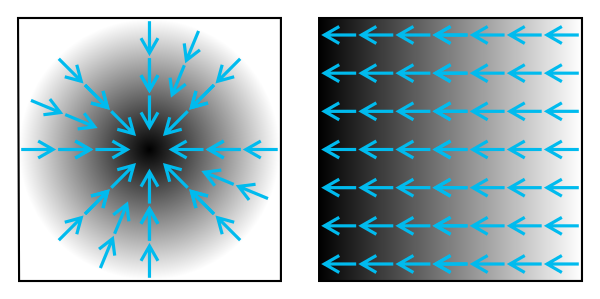
\includegraphics[height=3cm]{imageGradient}
	\caption{دو مثال از جهت‌گیری بردار‌های گرادیان در تصاویر}
	\label{gradImgEx}
\end{figure}
\subsection{در‌هم‌ریزی پوآسون}
در این قسمت، در‌هم‌ریزی پوآسون را به عنوان روشی برای ترکیب دو تصویر متفاوت در فضای گرادیان آورده‌ایم. تعریف مسئله و متغیر‌های مشخص‌شده در این قسمت از \cite{PoissonImageEditing} آورده شده‌است. ابتدا در شکل \ref{poissonSolve} متغیر‌ها را نمایش می‌دهیم و سپس به تعریف این متغیرها می‌پردازیم.
\begin{figure}[h!]
	\centering
	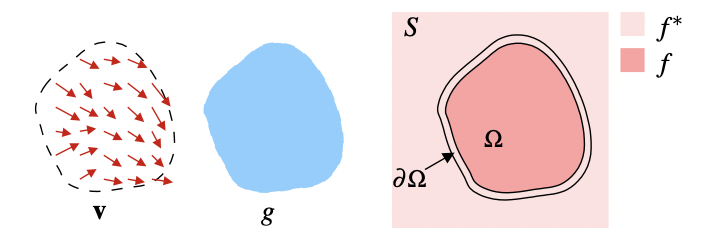
\includegraphics[height=3cm]{poissonSolve}
	\caption{نمایش متغیر‌های مورد استفاده در روش درهم‌ریزی پوآسون (از \cite{PoissonImageEditing})}
	\label{poissonSolve}
\end{figure}
در شکل \ref{poissonSolve}، متغیرها به این صورت تعریف می‌شوند:
\begin{itemize}
	\item 
	$g$ : تابع منبع
	\item 
	S : فضای مقصد
	\item 
	$\Omega$ : زیرمجموعه‌ای از فضای مقصد
	\item 
	$f$ : تابع درون‌یابی
	\item
	$f^*$ : تابع مقصد
	\item 
	\textbf{v} : میدان برداری (می‌تواند گرادیان g .باشد)
\end{itemize}
در مسئله‌ی درهم‌ریزی پوآسون، ما $f$ را طوری به دست می‌آوریم که بتواند هم مشخصات \lr{v} و هم مشخصات $f^*$ را حفظ کند. به این منظور یک مسئله‌ی بهینه‌سازی مطابق معادله‌ی \ref{variationalEq} تعریف می‌شود.
\begin{equation} \label{variationalEq}
	\min_f \iint_\Omega |\nabla f - \text{\textbf{v}} |^2 \quad \textrm{with} \quad f|_{\partial \Omega} = f^*|_{\partial \Omega} 
\end{equation}
به طوری که 
$\nabla f = \begin{bmatrix} \frac{\partial f}{\partial x} &  \frac{\partial f}{\partial y}\end{bmatrix}$ 
و 
$\text{\textbf{v}} = (u,v) = \nabla g$.

پاسخ معادله‌ی \ref{variationalEq} با پاسخ معادله‌ی زیر برابر خواهد بود:
\begin{equation} \label{poissonEq}
	\Delta f = \textrm{div}\ \text{\textbf{v}}\ \textrm{over}\ \Omega \quad \textrm{with} \quad f|_{\partial \Omega} = f^*|_{\partial \Omega} 
\end{equation}
به طوری که 
$\Delta f = \begin{bmatrix}\frac{\partial^2 f}{\partial x^2} + \frac{\partial^2 f}{\partial y^2}\end{bmatrix}$.
از طرف دیگر، داریم:
\begin{equation}
	\textrm{div}\ \text{\textbf{v}} = \frac{\partial u}{\partial x} + \frac{\partial v}{\partial y} = \frac{\partial^2 g}{\partial x^2} + \frac{\partial^2 g}{\partial y^2} = \Delta g
\end{equation}
که نشان می‌دهد با استفاده از این معادله‌ در حال یکسان‌سازی لاپلاس توابع \lr{$g$} و \lr{$f$} هستیم. این معادله، یک معادله پوآسون به همراه \gls{Dirichlet boundary conditions} است.
\newline
معادله‌ی \ref{poissonEq} پایه‌ی اصلی ویرایش تصاویر رنگی به روش پوآسون است. برای اجرای این روش در فضای رنگی، سه دفعه این معادله در سه کانال فضای رنگی انتخاب‌شده (لزومی بر \lr{RGB} بودن نیست)، به صورت مجزا اجرا می‌شود تا تصویر نهایی به دست آید.
\newline
با توجه به این موضوع که معادله‌ی \ref{poissonEq} را می‌توان به صورت مجزا برای هر پیکسل اجرا کرد، برای هر پیکسل مانند \lr{p}، می‌توان نوشت:
\begin{equation}
	\Delta f_p = \Delta g_p
\end{equation}
که با توجه به فیلتر پیچشی معرفی‌شده در بخش قبلی برای محاسبه‌ی لاپلاس در تصاویر، این معادله برای تصاویر به شکل زیر نوشته می‌شود:
\begin{equation}
	4f_p - \sum_{q \in N_p} f_q = 4g_p - \sum_{q \in N_p}  g_q
\end{equation}
که $N_p$ مجموعه‌ی همسایگی‌های پیکسل \lr{p} را نمایش می‌دهد. این معادله را می‌توان به صورت زیر نوشت:
\setcounter{MaxMatrixCols}{20}
\begin{equation} \label{linearPoisson}
	\begin{bsmallmatrix}0 & \ldots & 0 & -1 & 0 &  \ldots & -1 & 4 & -1 & 0 & \ldots & -1 & 0 & \ldots& 0\end{bsmallmatrix} 
	\begin{bsmallmatrix}f_1 \\ \vdots \\ f_{q1} \\ \vdots\\ f_{q2} \\ f_p \\ f_{q3} \\ \vdots \\ f_{q4} \\ \vdots \\ f_N \end{bsmallmatrix} = 
	\begin{bsmallmatrix}\Delta g_1 \\ \vdots \\ \Delta g_{q1} \\ \vdots\\ \Delta g_{q2} \\ \Delta g_p \\ \Delta g_{q3} \\ \vdots \\ \Delta g_{q4} \\ \vdots \\ \Delta g_N\end{bsmallmatrix}
\end{equation}
معادله‌ی \ref{linearPoisson} یک معادله خطی به شکل \lr{$Af = b$} است که به ازای هر پیکسل، یک سطر از ضرایب به بخش $A$ اضافه می‌شود. می‌توان این معادله را برای رسیدن به $f$، که تابع هدف ما و همان تابع درون‌یابی است، با روش‌های مختلف حل سیستم معادله‌های خطی به‌دست آورد. مشخص است ماتریس نهایی $A$، یک ماتریس $N*N$ خواهد بود. می‌توان نمایش داد این ماتریس همان ماتریس 
\lr{$(\nabla f)^T \nabla f$} 
و در نتیجه متقارن و \gls{Positive-Definite} است.
\subsection{واپیچش تصویر}
واپیچش در تصاویر زمانی اتفاق می‌افتد که خطوط صاف در تصویر، بعد از عکس‌برداری با دوربین، از صاف بودن خارج می‌شوند. واپیچش نوعی ابیراهی نوری است که اگرچه می‌تواند نامنظم باشد یا از الگوهای مختلف پیروی‌کند، اما اغلب به علت تقارن لنز تصویربرداری به طور شعاعی متقارن یا تقریبا متقارن است. این واپیچش‌های شعاعی معمولاً می توانند به عنوان واپیچش بشکه‌ای یا واپیچش بالشتکی طبقه‌بندی شوند، که در ادامه تعریف‌های این دو نوع واپیچش را آورده‌ایم. در شکل \ref{distortions} نیز می‌توان مثالی برای این دو واپیچش مشاهده کرد.
\begin{description}
	\item[واپیچش بشکه‌ای:]
در واپیچش بشکه‌ای، بزرگنمایی تصویر با فاصله‌گرفتن از مرکز تصویر کاهش می‌یابد. نتیجه‌ی ظاهری آن مانند تصویری است که به دور یک بشکه ترسیم شده‌است. لنزهای \gls{Fish-Eye} که نماهای نیمکره‌ای دارند، از این نوع واپیچش به عنوان راهی برای نمایش زوایای بیشتری از صحنه در تصویر محدود استفاده می‌کنند. در یک لنز برزگ‌نمایی، واپیچش بشکه‌ای در وسط تصویر ظاهر می‌شود و هر چه به کناره‌های تصویر نزدیک می‌شویم، این واپیچش بدتر خواهد‌شد.
	\item[واپیچش بالشتکی:]
در واپیچش بالشتکی، بزرگنمایی تصویر با فاصله‌گرفتن از مرکز تصویر افزایش می‌یابد. نتیجه‌ی قابل مشاهده این است که خطوطی که از مرکز تصویر عبور نمی‌کنند، به سمت داخل، یعنی مرکز تصویر، مانند یک بالشتک، خم می‌شوند.
\end{description}
\begin{figure}[h]
	\centering
	\subfloat[تصویر اصلی]{
\includegraphics[height=4cm]{distortions-1}\label{distortions:f1}}
	\qquad
	\subfloat[واپیچش بالشتکی]{
\includegraphics[height=4cm]{distortions-2}\label{distortions:f2}}
	\qquad
	\subfloat[واپیچش بشکه‌ای]{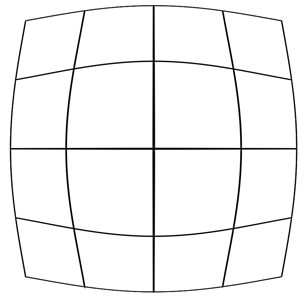
\includegraphics[height=4cm]{distortions-3}\label{distortions:f3}}
	\caption{دو نوع اصلی واپیچش در تصاویر}
	\label{distortions}
\end{figure}
\section{مروری بر مطالعات انجام‌شده}
در این قسمت تعدادی از پژوهش‌های مرتبط با هدف ما آورده شده‌است. این پژوهش‌ها در دو زمینه‌ی تولید بافت از یک تصویر و اتصال تصاویر برای تولید سراسرنما صورت گرفته‌اند. برای بررسی جامع پژوهش‌های انجام‌شده در زمینه‌ی تولید بافت از یک تصویر به \cite{jetchev2017texture} و \cite{survey2020} مراجعه کنید. این قسمت با استفاده از \cite{szeliski2011computer} نوشته شده است که سعی کردیم در طول مسیر پژوهش از این کتاب به عنوان مرجع اصلی استفاده کنیم.
\subsection{تولید بافت از یک تصویر} \label{texSynLit}
مسئله‌ی تولید بافت را می توان به صورت تولید بافت با استفاده از ورودی یک نمونه‌ی کوچک از آن، توصیف کرد. رویکردهای سنتی برای تولید بافت تلاش می‌کنند خروجی‌های تولید‌شده با طیف تصویر منبع مطابقت داشته باشند و در عین حال \gls{Structured Noise} ایجاد کنند. الگوریتم‌های تولید بافت از یک تصویر به‌طور متوالی پیکسل‌های بافت را برای جست‌وجوی همسایگی‌هایی در بافت منبع که مشابه تصویر فعلی تولید شده هستند، استفاده می‌کنند\cite{nonParam}. در اجرا، مشابه‌ترین همسایگی را در نمونه‌ی بافت پیدا می‌کنند و سپس تمام همسایه‌های دیگر را در فاصله
\lr{$d=(1+\epsilon)$} 
  با
\lr{$\epsilon=0.1$}  
  درنظر می‌گیرند. آنها همچنین پیکسل‌های مناسب برای ادامه‌ی تولید بافت را به صورت تصادفی و با وزن انتخاب‌شده با معیار فاصله‌ی d برای پیکسل‌های همسایگی مناسب، انتخاب می‌کنند.

برای تسریع این فرآیند و بهبود کیفیت ظاهری آن، \cite{treeVecQuant} این روش را با استفاده از فرآیند تولید \gls{Coarse-to-Fine} گسترش دادند، جایی که سطوح درشت‌تر هرم، که قبلاً تولید شده‌اند، نیز در طول یافتن پیکسل مناسب در نظر گرفته می‌شوند\cite{deBonet}. برای تسریع یافتن نزدیکترین همسایه، از \gls{Quantization} برداری با ساختار درختی استفاده می‌شود. یک نسخه بسیار سریع‌تر در جستجوی مشابه‌ترین پیکسل همسایه، الگوریتم به‌روزرسانی تکراری تصادفی \gls{Patch-Based} است که توسط \cite{patchMatch} توسعه داده شده است. محققین در
\cite{imageQuilting} 
روشی برای افزایش سرعت و بهبود ویژگی‌های ظاهری تصویر تولید‌شده‌ی نهایی پیشنهاد کردند. به جای تولید یک پیکسل در هر زمان، بلوک های مربعی که با یکدیگر هم‌پوشانی دارند برای استفاده در جست‌وجوی مشابه‌ترین بلوک با بافت تولید‌شده‌ تا به آن زمان استفاده می‌شوند. هنگامی که بلوک‌های مناسب انتخاب شدند، \gls{Seam} بین بلوک‌های همپوشانی جدید با استفاده از برنامه‌نویسی پویا تعیین می‌شود. از آنجا که این فرآیند شامل انتخاب تکه‌های کوچک و اتصال آن‌ها به یکدیگر است، آن‌ها سیستم خود را \gls{Image Quilting} می‌نامند.

ادامه‌ی پژوهش‌های انجام شده در این زمینه، به صورت خاص‌منظوره نسبت به هدف استفاده از بافت انجام شده‌اند. به طور مثال در زمینه‌ی پرکردن شکاف در تصویر، \cite{criminisiPerezInpaint} روشی را با استفاده از تولید بافت مبتنی بر نمونه ارائه می‌دهد که در آن، ترتیب ترکیب با مقادیر گرادیان در امتداد مرز منطقه تعیین می‌شود. \cite{wexlerIrani} نیز از روشی مشابه برای پر کردن شکاف در ویدئو‌ها استفاده می‌کند. در جدیدترین پژوهش‌ها تلاش‌شده با استفاده از یادگیری عمیق، روش‌هایی برای بهبود ویژگی‌های ظاهری تصویر تولید‌شده‌ی نهایی ارائه شود\cite{nazeri2019edgeconnect}\cite{yi2020contextual}. در تعدادی از این پژوهش‌ها، استخراج ساختار و گسترش بافت به ابعاد دلخواه، همگی توسط یک شبکه‌ عصبی با استفاده از لایه‌های پیچشی انجام شود\cite{gatys2015texture}\cite{risser2020optimal}.
\subsection{ترکیب تصاویر در فضای گرادیان}
بازسازی تصاویر از فضای گرادیان آن‌ها، از زمینه‌های قدیمی در بینایی ماشین است\cite{HornRV} که اولین استفاده‌ها از این روش در ثبات روشنایی\cite{Horn1974DeterminingLF}، شکل از سایه‌زنی\cite{shapeFromShading} و استریو فوتومتریک\cite{Woodham1994GradientAC} بوده است. ایده‌های مشابهی برای بازسازی تصاویر با استفاده از لبه‌های موجود در تصویر\cite{elderGoldberg}، از بین بردن سایه در تصاویر\cite{weissShadow} و جداسازی بازتاب نور از تصویر\cite{levinReflect1}\cite{levinReflect2} نیز استفاده شده است.

\cite{PoissonImageEditing}
 نشان می‌دهد چگونه می‌توان از بازسازی در فضای گرادیان برای ترکیب یک تصویر در تصویر دیگر استفاده کرد. به جای تکرار کردن مستقیم پیکسل‌ها، از تکرار مقادیر گرادیان تصاویر استفاده می‌شود. پیکسل‌ها در انتها با استفاده از حل کردن یک معادله‌ی پوآسون برای یکسان‌سازی محلی مقادیر گرادیان با توجه به شرایط مرزی دیریکله در ناحیه هم‌پوشانی محاسبه می‌شوند. در پژوهش‌های قدیمی‌تر، \cite{Peleg1981EliminationOS} یک تابع هموارساز معرفی می‌کند تا برای اطمینان از پایداری تصویر در ناحیه هم‌پوشانی از آن استفاده شود.

\cite{agarwala2004}
 این ایده را برای استفاده در مسئله‌ی ترکیب چند تصویر ورودی بسط داده است که دیگر صحبت از مقصد برای هموارسازی در ناحیه هم‌پوشانی معنا ندارد. در عوض، از گرادیان هر منبع در معادله‌ی پوآسون استفاده می‌شود و این معادله با توجه به \gls{Neumann boundary conditions} حل می‌شود. به جای حل مستقیم معادله پو‌آسون، در این روش از حداقل‌سازی یک مسئله‌ی متغیر استفاده می‌شود که در معادله‌ی \ref{agarwala} آمده است.
\begin{equation} \label{agarwala}
	\min_{C(x)} ||\nabla C(x) - \nabla \tilde{I}_{l(x)}(x)||^2
\end{equation} 
فرم گسسته‌ی این معادله را می‌توان با استفاده از تعدادی معادله‌ی قیود گرادیان به صورت زیر نوشت:
\begin{gather}
	C(x+\hat{i}) - C(x) = \tilde{I}_{l(x)}(x+\hat{i}) - \tilde{I}_{l(x)}(x) \qquad \textrm{and}\\
	C(x+\hat{j}) - C(x) = \tilde{I}_{l(x)}(x+\hat{j}) - \tilde{I}_{l(x)}(x) \qquad \quad
\end{gather}
که 
\lr{$\hat{i} = (1,0)$} 
و 
\lr{$\hat{j} = (0,1)$} 
بردارهای یکّه در جهت محور‌های $x$ و $y$ هستند. آن‌ها سپس این مسئله‌ی حداقل مربعات پراکنده را حل می‌کنند. از آنجایی که این سیستم معادلات فقط تا یک حد افزایشی تعریف شده است، در پژوهش از کاربر خواسته می‌شود مقدار یک پیکسل را مشخص کند. در عمل، انتخاب بهتر ممکن است جهت‌دهی جزءی راه‌حل به سمت بازتولید مقادیر رنگ اصلی تصویر نهایی باشد.

به منظور تسریع حل این سیستم خطی پراکنده، محققان در \cite{fattal} از \gls{Multigrid} استفاده می کنند، در حالی که پژوهش شرح داده‌شده از روش گرادیان استفاده می کند\cite{56188}\cite{10.1145/1141911.1142005}\cite{10.1145/2070781.2024211}\cite{10.1145/2461912.2461992}. پژوهش بعدی، \cite{10.1145/1275808.1276495} نشان می‌دهد که چگونه استفاده از یک نمایش \gls{Quadtree} برای راه‌حل می‌تواند محاسبات را با کاهش حداقلی دقت، تسریع کند. \cite{fastPoisson} بیان می‌کند ترکیب در فضای لگاریتمی، یا استفاده از جمع به جای ضرب، ترجیح داده می‌شود، زیرا مطابقت تصویر نهایی تولید‌شده با تفاوت‌های نوری بافت در ناحیه هم‌پوشانی بیشتر است. نتایج ترکیب تصاویر به‌دست‌آمده مطلوب است، اگرچه هنگام کپی کردن مقادیر گرادیان بزرگ در نزدیکی ناحیه هم‌پوشانی باید دقت شود تا \gls{Double Edge} ایجاد نشود.

کپی کردن گرادیان‌ها به طور مستقیم از تصاویر منبع پس از قرار دادن ناحیه هم‌پوشانی، تنها یک رویکرد برای ترکیب تصاویر در فضای گرادیان است. \cite{SeamlessStitching} چندین نوع مختلف از این رویکردها را بررسی می‌کند که آنها را 
\lr{Gradient-domain Image Stitching}
یا \lr{GIST} می‌نامند. تکنیک‌هایی که آنها بررسی می کنند، شامل \gls{Feathering} گرادیان‌ها از تصاویر منبع، و همچنین استفاده از \gls{L1-Norm} در انجام بازسازی تصاویر از فضای گرادیان، به جای استفاده از \gls{L2-Norm} مانند معادله \ref{agarwala} است. روش پیشنهادی آن‌ها بهینه سازی نُرم یک تابع هزینه‌ی پوشش‌گذاری بر روی گرادیان‌های تصویر اصلی (که \lr{GIST1-l1} می نامند) است. از آنجایی که بهینه‌سازی نُرم یک با استفاده از برنامه‌نویسی خطی می تواند کند باشد، آنها الگوریتم سریع‌تری را در یک چارچوب چندشبکه‌ای توسعه می‌دهند. مقایسه‌ی بصری بین رویکرد ترجیحی آنها و \cite{agarwala2004} نتایج مشابهی را نشان می‌دهد، در حالی که به طور قابل توجهی از الگوریتم‌های ترکیب هرمی و پوشش‌گذاری بهتر است.		% فصل دوم: مروری بر مطالعات انجام شده
% !TeX root=../main.tex

\chapter{روش تحقیق}
در این بخش روش ارائه‌شده را شرح می‌دهیم. در ابتدا تعریفی از مسئله‌ی مورد بررسی در این پژوهش و قیود در نظر گرفته‌شده برای ورودی را بیان می‌کنیم. در ادامه، پیش‌زمینه‌ی محاسباتی راه‌حل استفاده‌شده برای حل مسئله‌ی موردنظر را توضیح می‌دهیم. در انتها الگوریتم پیاده‌سازی‌شده در این روش به صورت مرحله‌به‌مرحله بیان می‌شود.
\section{تعریف مسئله و قیود}
\label{section_problem}
در این پژوهش، ما به دنبال ارائه‌ی یک روش برای حل مسئله‌ی تولید بافت از یک تصویر هستیم، که بر روی الگو‌های تکراری با ساختار پیچیده متمرکز است. برای مشخص کردن مسئله‌ای که به دنبال حل آن هستیم، یک تعریف از مسئله‌ی تولید بافت بیان می‌کنیم:
\begin{definition} \label{texSynProblem}
با استفاده از ورودی یک الگوی دو‌بعدی محدود، خروجی با ساختار یکسان ورودی، ویژگی‌های ظاهری یکسان و به طول و عرض دلخواه تولید شود. 
\end{definition}
این مسئله، یکی از مسائل قدیمی در زمینه‌ی بینایی ماشین بوده که راه‌حل‌های مختلفی با استفاده از روش‌های متفاوت برای آن ارائه‌شده‌است (بخش \ref{texSynLit}). در این پژوهش ما ورودی این مسئله را تنها یک تصویر درنظر می‌گیریم.

ما تلاش می‌کنیم برای طیفی از ورودی‌های خاص، مسئله‌ی \ref{texSynProblem} را حل کنیم. قیود مشخص‌شده برای ورودی، شرایط را برای استفاده از روش مورد نظر ما در حل مسئله فراهم می‌کنند و نتایج تنها برای ورودی‌هایی که این ویژگی‌ها را دارند تولید شده‌است. امکان دارد این روش برای ورودی‌ها با ویژگی‌های متفاوت نیز نتایج مورد قبولی تولید کند یا بتواند برای حل مسائل دیگری استفاده شود، اما این موضوع بررسی نشده ‌است. قیود در نظر گرفته‌شده برای ورودی‌ها در ادامه آمده است:
\begin{itemize}
\item 
الگوی ورودی از تکرار یک قطاع موجود در الگو تشکیل می‌شود.
\item 
تعداد تکرار‌های قطاع در الگو قابل شمارش و محدود است.
\item 
قطاع، ارتفاعی برابر با الگوی اصلی دارد.
\item 
خروجی تنها با استفاده از گسترش افقی تولید می‌شود.
\end{itemize}
\section{پیش‌زمینه محاسباتی} \label{conjGradExp}

در این بخش، الگوریتم \gls{Conjugate Gradient}، که در این روش استفاده می‌شود را شرح داده‌ایم. سیستم معادلات خطی که ماتریس آنها متقارن و مثبت معین است را می‌توان با استفاده از این روش به صورت \gls{Iterative} حل کرد. روش گرادیان مزدوج را می‌توان از دیدگاه‌های مختلف به دست آورد، از جمله روش جهت مزدوج برای بهینه سازی، و تغییر تکرارشونده Arnoldi/Lanczos برای مسائل ارزش ویژه. علیرغم تفاوت در رویکردهای آنها، این روش‌ها یک موضوع مشترک دارند، اثبات متعامد بودن باقیمانده‌ها و مزدوج شدن جهت‌های جستجو. این دو ویژگی برای توسعه‌ی فرمول مختصر روش گرادیان مزدوج بسیار مهم هستند.

می‌گوییم دو بردار غیر صفر u و v با یکدیگر مزدوج هستند (نسبت به \lr{A}) اگر:
\begin{equation} \label{conjGrad1}
	\textrm{u}^T\textrm{Av} = 0
\end{equation}
با توجه به اینکه ماتریس A یک ماتریس متقارن و مثبت‌معین است، قسمت چپ معادله‌ی \ref{conjGrad1} یک ضرب داخلی را مشخص می‌کند:
\begin{equation}
	\textrm{u}^T\textrm{Av} = \langle\textrm{u,v}\rangle_{\textrm{A}} := \langle\textrm{Au,v}\rangle = \langle\textrm{u,A}^T\textrm{v}\rangle = \langle\textrm{u,Av}\rangle
\end{equation}
دو بردار مزدوج هستند اگر و تنها اگر، نسبت به این ضرب داخلی بر هم عمود باشند. مزدوج بودن یک رابطه‌ی متقارن است؛ یعنی اگر u با v مزدوج باشد، v نیز با u مزدوج است.

در نظر می‌گیریم 
\lr{$P=\{\textrm{p}_0, ..., \textrm{p}_n\}$} 
یک مجموعه $n$ عضوی از بردار‌هایی است که دوبه‌دو نسبت به A مزدوج هستند (
\lr{$\textrm{p}_i^T\textrm{Ap}_j = 0$}
، برای هر $i$ نامساوی با $j$). در نتیجه $P$ یک پایه برای فضای برداری 
$\mathbb{R}^n$ 
خواهد بود و ما می‌توانیم پاسخ $x^*$ برای معادله‌ی خطی 
\lr{$\textrm{A}x = \textrm{b}$} 
را با استفاده از این پایه بنویسیم:
\begin{equation}
	x^* = \sum_{i=0}^n\alpha_i \textrm{p}_i \Rightarrow Ax^* = \sum_{i = 0}^{n} \alpha_i \textrm{A}\textrm{p}_i
\end{equation}
اگر دوطرف معادله را از سمت چپ با $\textrm{p}_k^T$ ضرب کنیم، خواهیم داشت:
\begin{equation}
	\textrm{p}_k^T\textrm{b} = \textrm{p}_k^T\textrm{A}x^* = \sum_{i = 0}^{n} \alpha_i \textrm{p}_k^T \textrm{Ap}_i = \sum_{i = 0}^{n} \alpha_i \langle \textrm{p}_k,\textrm{p}_i\rangle_{\textrm{A}} = \alpha_k \langle \textrm{p}_k,\textrm{p}_k \rangle_{\textrm{A}}
\end{equation}
و:
\begin{equation}
	\alpha_k = \frac{\langle \textrm{p}_k, b \rangle}{\langle \textrm{p}_k, \textrm{p}_k \rangle_{\textrm{A}}}
\end{equation}
که با استفاده از این معادله می‌توان ضرایب $x^*$ را در فضای معرفی‌شده به دست آورد. پس باید ابتدا $n$ بردار مزدوج پیدا کرد و سپس ضرایب آن‌ها را برای $x^*$ محاسبه کرد. 

روش بالا، یک روش مستقیم برای حل معادله خطی است که برای $n$ کوچک قابل استفاده است. می‌دانیم در زمینه‌ی تصاویر، مقدار $n$ بزرگ خواهد بود و استفاده از روش بالا بسیار هزینه‌ی بالایی دارد. اگر بردار‌های $\textrm{p}_k$ را با دقت و به درستی انتخاب کنیم، دیگر نیازی به استفاده از تمام این بردارها برای رسیدن به یک جواب مناسب $x^*$ نخواهیم داشت و می‌توانیم با استفاده از روش گرادیان مزدوج، به صورت تکرارشونده، به حل سیستم معادلات خطی بپردازیم. با در نظر گرفتن یک حدس اولیه مانند \lr{$x_0$} (می‌تواند ۰ باشد یا تخمینی از پاسخ نهایی)، در هر تکرار، ما به دنبال پاسخ مناسب خواهیم بود و به یک معیار نیاز داریم تا بدانیم به جواب مناسب، $x^*$، نزدیک می‌شویم یا خیر. این معیار را می‌توانیم با توجه به اینکه $x^*$ به حداقل رساننده‌ی یکتای تابع درجه دوم زیر است، به دست آوریم:
\begin{equation}
	f(x) = \frac{1}{2}x^T\textrm{A}x - x^T\textrm{b}
\end{equation}
وجود یک نقطه‌ی حداقل یکتا برای این تابع، با توجه به متقارن و مثبت معین بودن ماتریس هسین این تابع مشخص است، چون می‌دانیم ماتریس A این ویژگی را دارد و $\textrm{H}(f(x)) = \textrm{A}$. از طرف دیگر می‌دانیم در صورتی که $x^*$ یک نقطه‌ی حداقل‌کننده باشد، باید مشتق تابع را صفر کند. با توجه به اینکه 
$\nabla f(x) = \textrm{A}x - b$ 
در نتیجه این نقطه پاسخ سیستم معادلات خطی نیز خواهد بود.

با توجه به ویژگی‌های گفته‌شده، مناسب است بردار اول پایه
 $\textrm{p}_0$ 
 را برابر با منفی گرادیان $f$ در نقطه‌ی \lr{$x = x_0$} قرار دهیم. می‌دانیم گرادیان تابع برابر با \lr{$\textrm{A}x - b$} است؛ در نتیجه بردار اول پایه به صورت \lr{$\textrm{p}_0=\textrm{b}-\textrm{A}x_0$} می‌شود و دیگر بردار‌های پایه با گرادیان، مزدوج خواهند بود. با توجه به اینکه ما به دنبال صفر کردن \lr{$\textrm{A}x-\textrm{b}$} هستیم، می‌توانیم \lr{$p_0$} را \gls{Residual}‌ در گام اول بدانیم. به طور کلی می‌توان مانده ($r$) در گام $k$ را به صورت زیر در نظر گرفت:
 \begin{equation}
 	r_k = \textrm{b} - \textrm{A}x_k
 \end{equation}
همانطور که دیدیم، این مقدار برابر منفی گرادیان تابع در نقطه‌ی \lr{$x_k$} خواهد بود، در نتیجه روش \gls{Gradient Descent} باید در این جهت حرکت کند؛ با این تفاوت که ما باید مطمئن‌شویم جهت‌های حرکت نسبت به هم مزدوج باشند. برای این کار، ما می‌توانیم جهت بعدی را از مانده‌ی فعلی و تمام جهت‌های قبلی به دست آوریم:
 \begin{equation}
	\textrm{p}_k = r_k - \sum_{i<k} \frac{\textrm{p}_k^T \textrm{A} r_k}{\textrm{p}_i^T \textrm{A} \textrm{p}_i} \textrm{p}_i
\end{equation}
با توجه به این جهت، نقطه‌ی بعدی را با معادلات زیر به دست می‌آوریم:
\begin{gather}
	x_{k+1} = x_k + \alpha_k \textrm{p}_k\\
	\alpha_k = \frac{\textrm{p}_k^T (\textrm{b} - \textrm{A} x_k)}{\textrm{p}_k^T \textrm{A} \textrm{p}_k} = \frac{\textrm{p}_k^T r_k}{\textrm{p}_k^T \textrm{A} \textrm{p}_k}
\end{gather}
در انتها این الگوریتم برای حل سیستم معادلات خطی در الگوریتم \ref{alg:conjugate} آمده است.
\lr{
	\begin{algorithm}[h]
		\onehalfspacing
		\caption{Conjugate gradient method for solving linear equations system}
		\label{alg:conjugate}
		\SetKwBlock{Repeat}{repeat}{}
		\DontPrintSemicolon \SetNoFillComment
		$r_0 \gets \textrm{b} - \textrm{A}x$ \\
		if $r_0$ is sufficiently small, then return $x_0$ as the result \\
		$\textrm{p}_0 \gets r_0$ \\
		$k \gets 0$ \\
		\Repeat{
			$\alpha_k \gets \frac{r_k^T r_k}{\textrm{p}_k^T \textrm{A} \textrm{p}_k}$ \\
			$x_{k+1} \gets x_k + \alpha_k \textrm{p}_k$ \\
			$r_{k+1} \gets r_k - \alpha_k \textrm{A} \textrm{p}_k$ \\
			if $r_{k+1}$ is sufficiently small, then exit loop \\
			$\beta_k \gets \frac{r_{k+1}^T r_{k+1}}{r_k^T r_k}$ \\
			$p_{k+1} \gets r_{k+1} + \beta_k \textrm{p}_k$ \\
			$k \gets k + 1$
		} 
		\textbf{Return} $x_{k+1}$
	\end{algorithm}
}
\section{تولید بافت برای اشیاء با الگوی تکرارشونده}
در این بخش، ما روش خود را شرح می‌دهیم. ابتدا رفع واپیچش بشکه‌ای، که به عنوان یک مرحله‌ی پیش‌پردازش در روش ما پیاده‌سازی شده‌است، بیان می‌شود. سپس پیاده‌سازی اتصال تصاویر در فضای گرادیان با استفاده از معادله‌ی پو‌آسون به روش گرادیان مزدوج شرح داده می‌شود که برای این پیاده‌سازی از \cite{panoramaMaster} بهره می‌جوییم. پس از این بخش، روش کامل را توصیف و گام‌های رسیدن به خروجی از ورودی را مشخص می‌کنیم. در انتها نیز رابط گرافیکی پیاده‌سازی‌شده به طور خلاصه آورده ‌شده است.
\subsection{رفع واپیچش}
در این قسمت با استفاده از کتاب‌خانه‌ی \lr{OpenCV\cite{opencv_library}} رفع واپیچش در تصویر را اجرا می‌کنیم. با توجه به اینکه تصاویر الگو‌ها از سطح رویی جسم استخراج می‌شوند و معمولا این اجسام حالت مکعب‌مستطیلی ندارند، امکان وجود واپیچش در تصاویر الگو‌ها وجود دارد. برای رفع واپیچش از متد‌ \lr{cv2.undistort} در کتاب‌خانه‌ی \lr{OpenCV} استفاده می‌کنیم. روش اصلی این کار در \cite{opencvCamCalib} آمده است. ما در این قسمت، تفاوت‌های روش پیاده‌سازی‌شده با روش اصلی را بیان می‌کنیم. در روش اصلی، از صفحه‌ی شطرنجی برای استخراج ماتریس ویژگی‌های دوربین و ضرایب رفع واپیچش استفاده شده است. ماتریس ویژگی‌های دوربین به صورت زیر تعریف می‌شود:
\begin{equation}
	camera\ matrix\ =\ \begin{bmatrix}
		f_x & 0 & c_x \\
		0 & f_y & c_y \\
		0 & 0 & 1
	\end{bmatrix}
\end{equation}
که در این ماتریس، \lr{$(f_x,f_y)$} نشان‌دهنده‌ی فواصل کانونی و \lr{$(c_x,c_y)$} نمایش‌دهنده‌ی مراکز نوری دوربین هستند. خروجی دیگر نیز، ضرایب رفع واپیچش هستند که به صورت یک بردار‌ با ۴، ۵، ۸، ۱۲  یا ۱۴ عضو مشخص می‌شود. این دو ویژگی استخراج‌شده از تصاویر صفحات شطرنجی، ورودی‌های اصلی تابع \lr{cv2.undistort} در کنار تصویری است که می‌خواهیم رفع واپیچش را بر روی آن اجرا کنیم.

در این پیاده‌سازی ما باید حالتی را بوجود آوریم که بتوان به صورت دستی برای هر تصویر ورودی، با تغییر ضرایب رفع واپیچش و بدون دانستن ویژگی‌های دوربین، رفع واپیچش را اعمال کنیم. ما برای رفع نیاز به دانستن ماتریس ویژگی‌های دوربین، این ماتریس را در پیاده‌سازی به صورت زیر تعریف می‌کنیم:
\begin{equation}
	camera\ matrix\ =\ \begin{bmatrix}
		10 & 0 & W/2 \\
		0 & 10 & H/2 \\
		0 & 0 & 1
	\end{bmatrix}
\end{equation}
که در این ماتریس، \lr{$W$} و \lr{$H$} به ترتیب طول و ارتفاع تصویر ورودی هستند. با بررسی‌های انجام‌شده متوجه شدیم در صورت در نظر گرفتن بردار ضرایب رفع واپیچش با چهار عضو، عضو اول این بردار ضریبی است که با استفاده از آن می‌توان واپیچش‌های بشکه‌ای و بالشتکی را رفع کرد. در نتیجه با استفاده از \lr{OpenCV} یک رابط کاربری گرافیکی ساده توسعه داده شده است تا بتوان مقدار این ضریب را تغییر داد و نتایج رفع واپیچش را مشاهده کرد. در انتها، تصویر رفع واپیچش‌شده ذخیره می‌شود. برای عملیات ریاضی از  \lr{NumPy\cite{harris2020array}} استفاده شده‌است. این رابط کاربری گرافیک در بخش \ref{GUI} نمایش داده شده است.
\lr{
	\begin{algorithm}[h]
		\onehalfspacing
		\caption{Distortion Correction for an input image of choice}
		\label{alg:distCorrect}
		\DontPrintSemicolon \SetNoFillComment
		\KwIn{An input image, Img}
		$W \gets \textrm{Img.Width}$ \\
		$H \gets \textrm{Img.Height}$ \\
		$\textrm{distCoeffs} \gets [0.0, 0.0, 0.0, 0.0]$ \text{/* Initial Distortion Correction Coefficient */}\\
		$\textrm{camMat} \gets [[10, 0, W/2], [0, 10, H/2], [0, 0, 1]]$ \text{/* Camera Matrix */} \\
		setupTrackbars() \text{/* Setup Trackbars to Choose Coefficient */} \\
		\While{Keyboard key 'q' is not pressed}{
			$\textrm{distCoeffs}[0, 0] \gets \textrm{getTrackbarValue()}$ \\
			$\textrm{dst} \gets \textrm{\lr{cv2.undistort}}(\textrm{Img}, \textrm{camMat}, \textrm{distCoeff})$ \\
			$drawGridLines(dst)$ \text{/* Draw Grid Lines on Image for Guidance */} \\
			showImage(dst) \\
		}
		saveImage(dst) \\
	\end{algorithm}
}
\subsection{اتصال تصاویر در فضای گرادیان}
در این بخش، روش اتصال تصاویر در فضای گرادیان، را به صورت گام‌به‌گام شرح می‌دهیم. منظور از ارتفاع، اندازه‌ی تصویر در محور عمودی و منظور از طول، اندازه‌ی تصویر در محور افقی در نظر گرفته شده‌است. برای پیاده‌سازی این قسمت از زبان برنامه‌نویسی \lr{C++} استفاده می‌شود. تمام عملیات را درون یک تابع قرار می‌دهیم که ورودی این تابع، آرایه‌ای از تصاویر که باید به هم متصل شوند، شیفت هر تصویر در محور افقی و تعداد تصاویر است. برای انجام عملیات مشتق‌گیری از تصویر، همانطور که در بخش \ref{imageGradExp} توضیح داده‌شد، دو فیلتر پیچشی برای محور‌های افقی و عمودی به شکل زیر تعریف می‌کنیم:
\begin{equation}
	dx = [0, 0, -1, 1], \qquad dy = [1, -1, 0, 0]
\end{equation}
تصویر نهایی را به صورت یک آرایه دوبعدی با مقادیر صفر، ارتفاع برابر با ارتفاع تصویر اول و طول برابر با جمع آخرین شیفت و طول تصویر اول، تعریف می‌کنیم. در اولین گام، تصویر اول را در ابتدای این آرایه قرار می‌دهیم. حال برای هر تصویر درون آرایه‌ی تصاویر، به‌جز تصویر اول، شروع به اجرای حلقه می‌کنیم.

در ابتدا ناحیه‌ی هم‌پوشانی را بر روی تصویر فعلی با توجه به مقدار شیفت تصویر فعلی، مقدار شیفت تصویر قبلی و طول تصویر قبلی، محاسبه می‌کنیم. مقدار به‌دست آمده، نقطه‌ی شروع تصویر فعلی در تصویر نهایی با در نظر گرفتن هم‌پوشانی است. در این روش ما تلاش می‌کنیم مقدار درست تصویر فعلی را از خارج به داخل به صورت گام‌به‌گام، به تصویر نهایی منتقل کنیم. برای اینکار ابتدا ردیف بالا، ردیف پایان و ستون آخر تصویر را در مکان مناسب بر روی تصویر نهایی قرار می‌دهیم و می‌دانیم ستون اول با ستون آخر تصویر قبلی باید یکسان باشد. بعد از قرار دادن این سطر و ستون‌ها، حال می‌توانیم روند اصلی را برای تصویر فعلی آغاز کنیم. حد بالای تعداد تکرار را برابر ۱۰۰۰ قرار می‌دهیم و یک ماتریس برای مقادیر مانده (با توجه به الگوریتم گرادیان مزدوج که در بخش \ref{conjGradExp} شرح دادیم) با ابعاد برابر با تصویر فعلی، به نام \lr{res}، آماده می‌کنیم.

حال شروع به اجرای حلقه بر روی تمام مقادیر تصویر فعلی (به جز سطر و ستون‌های حاشیه‌ای) می‌کنیم. مقدار مانده برای هر پیکسل را در ابتدا صفر می‌کنیم، سپس بر روی مقادیر $dx$ و $dy$ مشخص‌شده، اجرای یک حلقه‌ی‌ دیگر را آغاز می‌کنیم. درون این حلقه‌ی داخلی، ابتدا طول و ارتفاع پیکسل همسایگی را با توجه به طول و ارتفاع پیکسل فعلی و مقادیر $dx$ و $dy$ فعلی، مشخص می‌کنیم. حال مقدار مانده‌ی پیکسل فعلی را برابر با مجموع اختلاف مقدار پیکسل فعلی و مقدار پیکسل همسایگی در تصویر فعلی و مقدار پیکسل همسایگی و پیکسل فعلی در تصویر نهایی قرار می‌دهیم. در واقع با این کار ما مقدار \lr{$\textrm{b}-\textrm{A}x$} را محاسبه می‌کنیم و مقدار اولیه‌ی ماتریس مانده‌ها را برابر با آن قرار می‌دهیم. مقدار b همان گرادیان تصویر نهایی است که اینجا با استفاده از $dx$ و $dy$ محاسبه می‌شود.

سپس یک ماتریس جدید برای مقادیر $p$‌(جهت حرکت گرادیان) با نام \lr{search\_p} تعریف می‌کنیم و مقدار اولیه آن را برابر با ماتریس مانده‌ها قرار می‌دهیم. در ادامه، شروع به اجرای حلقه با حد بالای تعداد تکرار می‌کنیم، البته در میان اجرای این حلقه، در صورتی که میزان خطا از حد دلخواه کمتر شد، از حلقه خارج می‌شویم. یک ماتریس موقت با نام \lr{vec} تعریف می‌کنیم که ابعادی برابر با تصویر فعلی دارد و مقدار اولیه‌ی آن صفر است. با اجرای حلقه بر روی تمام پیکسل‌ها و مقادیر همسایگی هر پیکسل، مقدار این ماتریس را برای آن پیکسل، اگر همسایگی پیکسل درون ناحیه‌ی مناسب (درون تصویر به جز سطر‌های اول و آخر، ستون آخر و ستون ابتدای ناحیه هم‌پوشانی) باشد، با اختلاف مقدار ماتریس جهت پیکسل و همسایگی و در صورتی که همسایگی خارج از ناحیه مناسب باشد، با مقدار ماتریس جهت پیکسل جمع می‌کنیم. با این کار ما در واقع ماتریس \lr{$\textrm{A}\textrm{p}$} را تشکیل می‌دهیم.

حال باید مقدار $\alpha_k$ را محاسبه کنیم. برای این کار صورت و مخرج کسر محاسبه‌ی $\alpha_k$ را جدا می‌کنیم. این صورت و مخرج هر کدام به صورت بردار‌های سه عضوی تعریف می‌شوند (سه کانال رنگی) که مقدار ابتدایی صفر دارند. با حلقه زدن بر روی ناحیه‌ی مناسب تصویر، مقادیر صورت و مخرج را هر بار با مقادیر مناسب جمع می‌کنیم. مقدار مناسب هر تکرار برای صورت برابر با ضرب مقدار ماتریس مانده در آن نقطه با خودش (معادل \lr{$r_k^T r_k$}) و مقدار مناسب برای مخرج نیز برابر با ضرب ماتریس جهت و ماتریس موقت \lr{vec} (معادل \lr{$\textrm{p}_k^T \textrm{A} \textrm{p}_k$}) است. در انتها صورت بر مخرج تقسیم می‌شود تا مقدار نهایی \lr{$\alpha_k$} محاسبه شود.

پس از محاسبه‌ی \lr{$\alpha_k$}، حال می‌توانیم مقادیر تصویر نهایی، مقادیر ماتریس مانده و مقدار \lr{$\beta_k$} برای محاسبه‌ی مقادیر جدید ماتریس جهت را محاسبه کنیم. برای این کار، ابتدا دو بردار صورت و مخرج برای \lr{$\beta_k$} را به صورت دو بردار سه عضوی برابر با صفر تعریف می‌کنیم. با توجه به اینکه صورت کسر محاسبه‌ی \lr{$\alpha_k$} با مخرج کسر محاسبه‌ی \lr{$\beta_k$} برابر است، بردار مخرج را برابر با بردار صورت کسر محاسبه‌ی \lr{$\alpha_k$} قرار می‌دهیم. حال بر روی پیکسل‌های ناحیه‌ی مناسب اجرای حلقه را آغاز می‌کنیم. در حلقه، مقدار تصویر نهایی متناظر با آن پیکسل را با مقدار \lr{$\alpha_k$} ضرب در ماتریس جهت آن پیکسل، جمع می‌کنیم (معادل \lr{$x_k + \alpha_k \textrm{p}_k$}). سپس از مقدار ماتریس مانده‌ی آن پیکسل، به اندازه‌ی \lr{$\alpha_k$} ضرب در ماتریس موقت آن پیکسل، کم می‌کنیم (معادل \lr{$r_k - \alpha_k \textrm{A} \textrm{p}_k$}). بعد از این محاسبات، مقدار صورت \lr{$\beta_k$} را با ضرب ماتریس مانده‌ی به‌روز‌شده‌ی پیکسل در خودش، جمع می‌کنیم (معادل تشکیل \lr{$r_{k+1}^T r_{k+1}$}) بعد از خارج شدن از لوپ، صورت $\beta_k$ را بر مخرج آن تقسیم می‌کنیم تا مقدار نهایی $\beta_k$ را داشته باشیم. حال می‌توانیم با استفاده از این مقدار و با اجرای حلقه بر روی پیکسل‌ها، مقدار ماتریس جهت را با مساوی قرار دادن آن با جمع مقدار ماتریس مانده‌ی به‌روز‌شده و ضرب $\beta_k$ در مقدار ماتریس جهت قبلی، به‌روز‌ کنیم. 

در انتها بیشترین مقدار بردار $\beta_k$ را به عنوان خطای فعلی در نظر می‌گیریم. با توجه به اینکه تعریف $\beta_k$ به نوعی نسبت تغییرات مانده‌ها در هر گام را نمایش می‌دهد، این کار به نظر منطقی است و نتایج مناسبی را هم تولید می‌کند. حال اگر این مقدار خطا از یک حد (در این پیاده‌سازی مقدار آن $1$ در نظر گرفته شده) کمتر بود، از حلقه خارج می‌شویم و سراغ تصویر بعدی می‌رویم. بعد از اتمام انجام این محاسبات، تصویر نهایی بازگردانده می‌شود. گام‌های اجرای این تکنیک در الگوریتم \ref{alg:fusion} آورده شده‌است.
\lr{
	\begin{algorithm}[h!]
		\caption{Poisson Blend in Gradient Domain}
		\label{alg:fusion}
		\DontPrintSemicolon\SetNoFillComment
		\SetKwBlock{Begin}{Begin}{}
		\SetAlgoLined
		\SetKwFunction{procedureName}{\textbf{blendPoisson}} 
		\SetKwProg{myalg}{procedure}{}{}    
		\myalg{\procedureName{%
				pic[], imgCount, shift[]%
		}}{
			$dx \gets [0, 0, -1, 1]$ \\
			$dy \gets [1, -1, 0, 0]$ \\
			$\textrm{fin} \gets \textrm{zeroMatrix}(\textrm{pic}[0].rows,\ \textrm{shift}[\textrm{imgCount} - 1] + \textrm{pic}[0].cols)$ \\
			\ForEach{$\textrm{pixel}(x,y)$ \textbf{in} $\textrm{pic}[0]$}{
				$\textrm{fin}(x, y) = \textrm{pixel}$
			}
			\For{$i \gets 1$ \KwTo imgCount}{
				$\textrm{ROI} \gets \textrm{pic}[i][1:-2,\ overlap:-2,\ :]$ \\
				$\textrm{overlap} \gets \textrm{shift}[i-1] + \textrm{pic}[i-1].cols - \textrm{shift}[i]$ \\
				\For{$y \gets \textrm{overlap}$ \KwTo $\textrm{pic}[i].cols$}{
					$\textrm{fin}(0, y + \textrm{shift}[i]) \gets \textrm{pic}[i](0, y)$ \\
					$\textrm{fin}(\textrm{pic}[i].rows - 1, y + \textrm{shift}[i]) \gets \textrm{pic}[i](\textrm{{}pic}[i].rows - 1, y)$
				}
				\For{$x \gets 0$ \KwTo $\textrm{pic}[i].rows$}{
					$\textrm{fin}(x, \textrm{pic}[i].cols - 1 + \textrm{shift}[i]) \gets \textrm{pic}[i](x, \textrm{pic}[i].cols - 1)$
				}
				$T \gets 1000$ \\
				$\textrm{res} \gets \textrm{zeroMatrix}(\textrm{pic}[i].rows,\ \textrm{pic}[i].cols)$ \\
				\ForEach{$\textrm{neighbor}(nx,ny)$ \textbf{of} $\textrm{pixel}(x,y)$ \textbf{in} $\textrm{ROI}$}{
					$\textrm{res}(x, y) \gets \textrm{res}(x,y) + \textrm{pic}[i](x, y) - \textrm{pic}[i](nx, ny)$ \\
					$\textrm{res}(x, y) \gets \textrm{res}(x,y) + \textrm{fin}(nx, ny + \textrm{shift}[i]) - \textrm{fin}(x, y + \textrm{shift}[i])$
				}
				$\textrm{searchP} \gets \textrm{res}.clone()$ \\
			}
		}{}
	\end{algorithm}
	\begin{algorithm}[h!]
		\setcounter{AlgoLine}{20}
		\SetKwBlock{Begin}{}{end}
		\SetKwProg{Loop}{LOOP}{}{}
		\Begin{
			\For{$k \gets 0$ \KwTo $T$}{
				$\textrm{vec} \gets \textrm{zeroMatrix}(\textrm{pic}[i].rows,\ \textrm{pic}[i].cols)$ \\
				\ForEach{$\textrm{neighbor}(nx,ny)$ \textbf{of} $\textrm{pixel}(x,y)$ \textbf{in} $\textrm{ROI}$}{
					\eIf{neighbor in ROI}{
						$\textrm{vec}(x, y) = \textrm{vec}(x, y) + \textrm{searchP}(x, y) - \textrm{searchP}(nx, ny)$
					}{
						$\textrm{vec}(x, y) = \textrm{vec}(x, y) + \textrm{searchP}(x, y)$
					}
				}
				$\alpha_{k1} \gets \alpha_{k2} \gets [0, 0, 0]$ \\
				\ForEach{$\textrm{pixel}(x,y)$ \textbf{in} $\textrm{ROI}$}{
					$\alpha_{k1} = \alpha_{k1} +  \textrm{res}(x, y).mul(\textrm{res}(x, y))$ \\
					$\alpha_{k2} = \alpha_{k2} +  \textrm{searchP}(x, y).mul(\textrm{vec}(x, y))$
				}
				$\alpha_k = \alpha_{k1} / \alpha_{k2}$ \\
				$\beta_{k1},\ \beta_{k2} \gets [0, 0, 0],\ \alpha_{k1}$ \\
				\ForEach{$\textrm{pixel}(x,y)$ \textbf{in} $\textrm{ROI}$}{
					$\textrm{fin}(x, y + \textrm{shift}[i]) = \textrm{fin}(x, y + \textrm{shift}[i]) + \alpha_k.mul(\textrm{searchP}(x, y))$ \\
					$\textrm{res}(x, y) = \textrm{res}(x, y) - \alpha_k.mul(\textrm{vec}(x, y))$ \\
					$\beta_{k1} = \beta_{k1} + \textrm{res}(x, y).mul(\textrm{res}(x, y))$
				}
				$\beta_k = \beta_{k1} / \beta_{k2}$ \\
				\ForEach{$\textrm{pixel}(x,y)$ \textbf{in} $\textrm{ROI}$}{
					$\textrm{searchP}(x, y) = \textrm{res}(x, y) + \beta_k.mul(\textrm{searchP}(x, y))$ 
				}
				\If{$max(\beta_k) < 1$}{break}
			}
			\textbf{Return} fin
		}
	\end{algorithm}
}
\subsection{روش نهایی}
در این قسمت، ما روش نهایی را ارائه می‌دهیم که از تکنیک معرفی‌شده در قسمت قبل برای تولید بافت استفاده می‌کند. این روش نیز به صورت یک تابع با استفاده از زبان برنامه‌نویسی \lr{C++} پیاده‌سازی شده است و برای اجرای کامل روش، از آن استفاده می‌شود.

در تابع پیاده‌سازی، که \lr{repBlend} نام دارد، ورودی‌ها شامل قطاع الگو و تعداد تکرار این قطاع در الگو است. در ابتدا قطاع دریافت شده دو بار تکرار می‌شود و سه قطاع تکراری درون یک آرایه قرار می‌گیرند. در تابع باید آرایه‌ی مقادیر شیفت افقی الگو‌ها نیز آماده شوند تا بتوان از تابع پیاده‌سازی‌شده برای ترکیب تصاویر استفاده کرد. تعداد این مقادیر شیفت باید برابر با تعداد تصاویر درون آرایه باشد. مقدار اول شیفت که برای تکرار اول قطاع است، برابر با صفر خواهد بود. این مقدار در ادامه با توجه به طول تصویر و اندازه‌ی ناحیه هم‌پوشانی، که در این پیاده‌سازی برابر با $2$ در نظر گرفته شده است، مشخص می‌شود که برابر 
\lr{$(\textrm{image}.cols - 2) * i$} 
خواهد بود که $i$، شماره‌ی تکرار قطاع است و در این مرحله از $0$ تا $2$ خواهد بود. پس از آماده‌سازی این دو آرایه، تعداد تکرار تصاویر را برابر با $3$ قرار می‌دهیم و به عنوان ورودی به تابع اتصال تصاویر می‌دهیم. خروجی پس از استخراج بریده می‌شود تا تنها قطاع وسط را داشته باشیم. ناحیه‌ی موردنظر، دو پیکسل از چپ و دو پیکسل از راست کوچک‌تر از قطاع ورودی اولیه خواهد بود و از هر دو طرف به مقدار خوبی هموار شده است.

در مرحله‌ی بعدی، این قطاع استخراج‌شده پس از یک بار هموار‌سازی، به تعداد ورودی داده‌شده به تابع برای تکرار، درون آرایه قرار می‌گیرد. میزان شیفت قطاع‌ها نیز متناسب با تصاویر، با همان مقدار 
\lr{$(\textrm{image}.cols - 2) * i$} 
انتخاب می‌شود، مقدار $i$ در این گام از صفر تا یکی کمتر از تعداد مشخص‌شده‌ی تکرار تصاویر برای تابع است. همانطور که مشخص است، ناحیه‌ی همسایگی در این قسمت هم برابر با دو پیکسل است. پس از آماده‌سازی این دو آرایه، آرایه‌ها با تعداد تکرار قطاع نهایی مشخص‌شده، به تابع اتصال تصاویر داده می‌شوند. تصویر به‌دست آمده از تابع اتصال تصاویر، بافت نهایی تولید‌شده با استفاده از روش ما خواهد بود. تمام گام‌های این روش در الگوریتم \ref{alg:final} آورده شده است.
\lr{
	\begin{algorithm}[h!]
		\caption{Final algorithm presented}
		\label{alg:final}
		\DontPrintSemicolon\SetNoFillComment
		\SetAlgoLined
		\SetKwFunction{procedureName}{\textbf{repBlend}} 
		\SetKwProg{myalg}{procedure}{}{}
		\myalg{\procedureName{%
				imageSlice, repCount%
		}}{
			$\textrm{pic} : \textrm{Array of matrices}$ \\
			$\textrm{shift} : \textrm{Array of numbers}$ \\
			\For{$i \gets 0$ \KwTo $3$}{
				$\textrm{pic}[i] = \textrm{imageSlice}.clone()$ \\
				$\textrm{shift}[i] = (\textrm{imageSlice}.cols - 2) * i;$
			}
			$fin \gets \textrm{blendPoisson(pic, \lr{3}, shift)}$ \text{/* Presented in } \\
			$ROI \gets (\textrm{imageSlice}.cols + 2, 0, \textrm{imageSlice}.cols - 4, \textrm{imageSlice}.rows)$ \\
			$\textrm{pic}[0] \gets fin[ROI]$ \\
			\For{$i \gets 0$ \KwTo $\textrm{repCount}$}{
				$\textrm{pic}[i] = \textrm{pic}[0].clone()$ \\
				$\textrm{shift}[i] = (\textrm{pic}[0].cols - 2) * i;$
			}
			$fin \gets \textrm{blendPoisson(pic, \textrm{repCount}, shift)}$ \\
			\textbf{Return} $fin$
		}{}
	\end{algorithm}
}
\subsection{رابط کاربری گرافیکی}
\label{GUI}
برای ساده‌‌تر کردن استفاده از الگوریتم پیاده‌سازی‌شده، یک رابط کاربری گرافیکی با استفاده از زبان برنامه‌نویسی \lr{Python}، با ورژن \lr{$3.9.9$}، توسعه داده شده‌است. با استفاده از این رابط کاربری می‌توان تصویر ورودی را انتخاب کرد، تصویر را در صورت برش داد، تعداد تکرار قطاع در بافت نهایی را انتخاب کرد و نام پوشه‌ی موردنظر برای ذخیره‌سازی تصاویر تولید‌شده را مشخص کرد. تصاویر ذخیره‌شده در حین اجرا شامل تصویر اولیه‌ی الگو، تصویر بریده‌شده‌ی الگو و تصویر بافت نهایی تولید‌شده است. تصویری از این رابط کاربری در شکل \ref{gui:f1} آمده است. رابط کاربری دیگری که توسعه‌ داده شده، برای بخش رفع واپیچش است که در آن می‌توان ضریب رفع واپیچش را در کنار برش تصویر از بالا و پایین انجام داد. ظاهر این رابط کاربری در شکل \ref{gui:f2} آمده است.

تابع اصلی مشخص شده در بخش قبلی نیز با استفاده از این رابط کاربری اجرا می‌شود. برای استفاده از تابع، که با زبان برنامه‌نویسی \lr{C++} نوشته شده در \lr{Python}، از کتاب‌خانه‌ی 
\lr{PyBind\cite{pybind}} 
استفاده شده‌است که می‌توان با استفاده از آن کد‌های \lr{C++} را به فایل‌های قابل استفاده در \lr{Python} تبدیل کرد. این کد‌ها با استفاده از \gls{Compiler} با نام \lr{$g++11$} گرد‌آوری می‌شوند. نتایج نشان می‌دهند استفاده از کد پیاده‌سازی‌شده بعد از گرد‌آوری از \lr{Python}، سرعت بالاتری از اجرای کد مستقیم \lr{C++} دارند.

\begin{figure}[htbp]
	\centering
	\subfloat[روش ارائه‌شده]{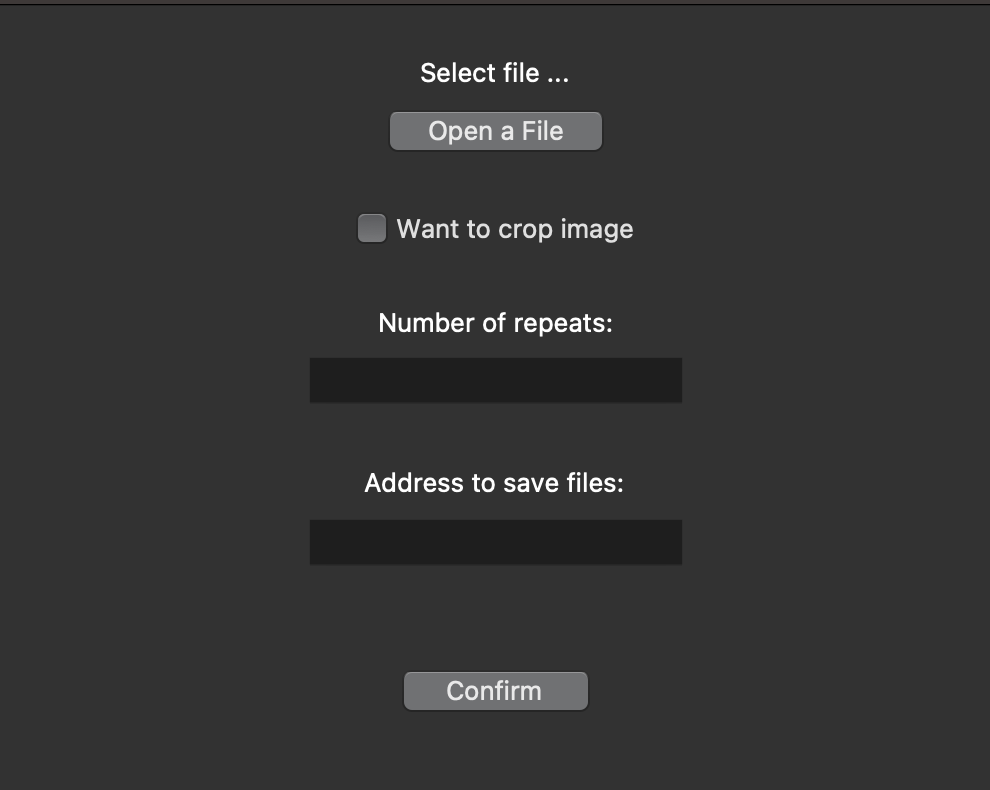
\includegraphics[height=5cm]{GUI-1}\label{gui:f1}}
	\qquad
	\subfloat[رفع واپیچش]{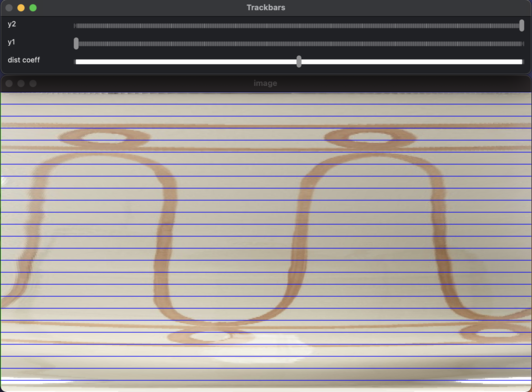
\includegraphics[height=5cm]{GUI-2}\label{gui:f2}}
	\caption{دو رابط کاربری گرافیکی توسعه داده‌شده}
	\label{gui}
\end{figure}






		% فصل سوم: روش تحقیق
% !TeX root=../main.tex

\chapter{نتایج}
\label{section_results}
در این قسمت با استفاده از تصاویر اشیاء مختلف، عملکرد روش خود را نمایش دادیم. برای استخراج الگوی رویی اشیاء و ساخت هندسه‌ی سه‌بعدی جسم، از الگوریتم رویه دورانی\cite{SMH.Hosseini} استفاده کردیم. در این الگوریتم بعد از مشخص کردن نقاط حاشیه‌ای شیء در تصویر ورودی، مدل سه‌بعدی تولید می‌شود. ما با ذخیره کردن الگو‌ی استخراج‌شده از سطح جسم، که به صورت تقریبی رفع واپیچش شده و به شکل یک مستطیل گشترش می‌یابد، از آن به عنوان ورودی الگوریتم خود استفاده می‌کنیم. خروجی الگوریتم را که بافت کامل مدل سه‌بعدی است را نیز با استفاده از همان الگوریتم بر روی مدل سه‌بعدی نگاشت کردیم.

ابتدا عملکرد روش خود را در مقایسه با تعدادی از الگوریتم‌های دیگر برای تولید بافت مقایسه کردیم. به این علت که تصاویر بافت‌های تولید‌شده باید به اندازه‌ی کافی بزرگ باشند تا ویژگی‌های ظاهری آن‌ها مشخص شود، نتایج در کنار هم نیامده‌اند و نتایج هر الگوریتم تنها در بخش خود آمده است. بافت‌ها نیز به نسبت طول به عرض تقریبا یکسانی تغییر اندازه داده شده‌اند تا بهتر دیده‌شوند. بعد از این قسمت، نتایج روش خود را در تولید بافت برای بازسازی سه‌بعدی با یک تصویر را نمایش داده‌ایم.

داده‌های نمایش داده‌شده برای نتایج به دست آمده، شامل تصویر ورودی شیء، الگوی رویی استخراج‌شده از تصویر شیء، قطاع تکرارشونده‌ی الگوی شیء، بافت نهایی تولید‌شده و مدل سه‌بعدی نهایی بعد از نگاشت بافت بر روی هندسه‌ی مدل می‌باشد. روش بر روی سیستم با پردازنده \lr{Apple M1 Pro} به همراه 
 \lr{16 GB}
 رم اجرا می‌شود و جدول زمانی اجرا در انتها‌ی بخش نتایج آورده شده‌است.
\section{مقایسه با روش‌های دیگر}

در این قسمت بافت تولید‌شده با استفاده از روش خود و تعدادی دیگر از روش‌ها را نمایش داده و مقایسه کرده‌ایم. برای این قسمت دو ورودی انتخاب شد که برای بعضی از الگوریتم‌ها از ورودی شکل \ref{compInputs:f1} و برای بقیه از شکل \ref{compInputs:f2} استفاده کردیم، اما برای مقایسه‌ی مناسب، بافت تولید شده از هر دو ورودی با استفاده از الگوریتم خودمان را نمایش دادیم.

در هر زیربخش، خروجی الگوریتم‌های مختلف را نمایش دادیم و آن را تحلیل می‌کردیم. در انتها نیز در یک جمع‌بندی کلی، تمام خروجی‌ها را نسبت به هم مقایسه شده و به تحلیل نتایج پرداختیم.

\begin{figure}[h]
	\centering
	\subfloat[]{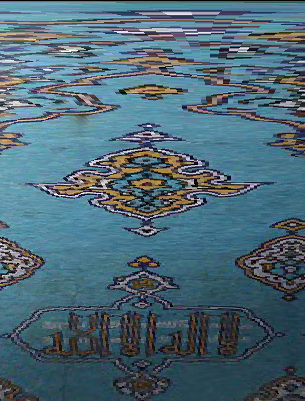
\includegraphics[height=4cm]{comparison-1}\label{compInputs:f1}}
	\qquad
	\subfloat[]{
\includegraphics[height=4cm]{comparison-2}\label{compInputs:f2}}
	\caption{قطاع‌های استفاده‌شده برای مقایسه}
	\label{compInputs}
\end{figure}


\subsection{ادغام تصاویر در فضای گرادیان} \label{imageFusion}
در این قسمت از 
\lr{Multi-exposure and multi-focus image fusion in gradient domain\cite{paul2016multi}}
برای تولید بافت استفاده شد. این الگوریتم با هدف گسترش تصویر پیاده‌سازی‌ نشده و برای ادغام تصاویر یک صحنه استفاده می‌شود. برای اجرای این الگوریتم متناسب با هدف ما، باید ورودی‌ها را به فرمت مناسبی آماده می‌کردیم. تصاویر ورودی به تعداد مناسب تکرار الگو ساخته شد و هر قطاع در یک تصویر جدا قرار گرفت. ورودی‌های تولید‌شده از قطاع از لحاظ افقی با قطاع تصویر قبلی و بعدی خود تعداد شش پیکسل \gls{Overlap} دارد که برای اجرای الگوریتم نیاز بوده است. وجود ناحیه‌های هم‌پوشانی بین تصاویر ورودی قطاع برای اجرای درست الگوریتم الزامی است. بعد از به دست آوردن خروجی از الگوریتم، قسمت هم‌پوشانی تیره‌تر از نواحی دیگر بافت خواهد بود. این قسمت‌ها در انتها حذف می‌شود تا بافت نهایی تولید شود.

نمونه‌ی ورودی مناسب برای اجرای الگوریتم با سه قطاع در شکل \ref{properInputs1} آمده است. حاشیه‌های دور تصاویر برای نمایش مناسب رنگ سفید قرار داده شده است و جزو تصاویر نیستند. هر تصویر در نواحی دیگر به جز قطاع، یک رنگ ثابت خواهد بود. این رنگ می‌تواند سفید، خاکستری (دقیقا میانه‌ی سفید و سیاه) و سیاه باشد. نتایج نشان داد استفاده از رنگ سفید بهترین نتیجه را داشت.
\setlength{\fboxsep}{0pt}%
\begin{figure}[h!]
	\centering
	\subfloat[]{\fbox{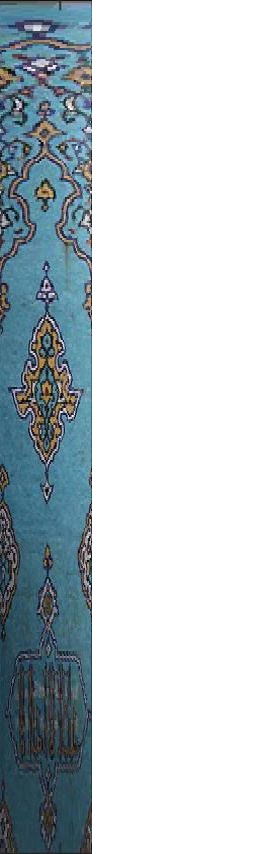
\includegraphics[height=4cm]{comparison-3}\label{properInputs1:f1}}}
	\qquad
	\subfloat[]{\fbox{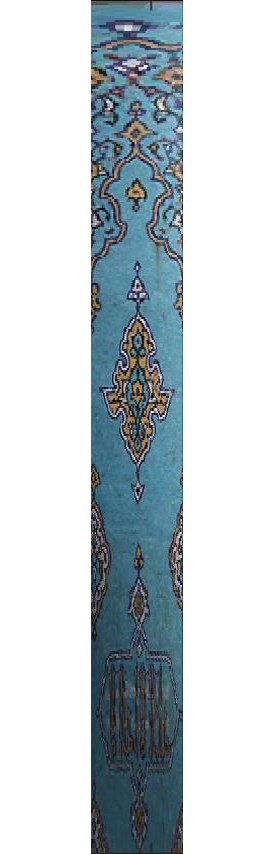
\includegraphics[height=4cm]{comparison-4}\label{properInputs1:f2}}}
	\qquad
	\subfloat[]{\fbox{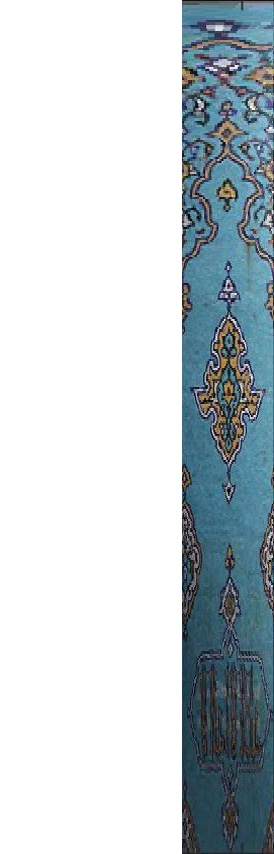
\includegraphics[height=4cm]{comparison-5}\label{properInputs1:f3}}}
	\caption{ورودی‌های مناسب برای الگوریتم ادغام تصاویر در فضای گرادیان}
	\label{properInputs1}
\end{figure}

 در شکل \ref{grayResult} نتایج تولید شده با استفاده از رنگ خاکستری برای نواحی غیر قطاع نمایش داده شده است. می‌توان از این خروجی نتیجه گرفت که چون رنگ خاکستری آنقدر متفاوت با رنگ خود قطاع نبوده است، الگوریتم تغییر مناسبی در رنگ و شدت نور قطاع ایجاد نکرده و شدت نور و رنگ در طول قطاع به ظاهر مناسبی دست پیدا نکرده است. این نتیجه هر چه از رنگ سفید دور می‌شویم، بیشتر مشاهده می‌شود. در نتیجه برای تولید نتایج مناسب با استفاده از این روش، از رنگ سفید برای نواحی غیرقطاع ورودی استفاده شده است. 
\begin{figure}[h!]
	\centering
	
\includegraphics[height=5cm]{comparison-6}
	\caption{خروجی الگوریتم ادغام تصاویر با استفاده از رنگ خاکستری برای نواحی قیر غطاع}
	\label{grayResult}
\end{figure}

در ابتدا با استفاده از ورودی‌های مشابه با قالب شکل \ref{properInputs1}، ورودی‌ها را برای دوازده تکرار قطاع آماده کردیم و این تصاویر را به الگوریتم دادیم تا نتایج را تولید کنیم. نتایج تولید شده در شکل \ref{twelveRep} آمده است. مشخص است الگوریتم در یکسان‌سازی شدت نور عملکرد مناسبی داشته و برای یکسان‌سازی رنگ قطاع، آن را روشن‌تر کرده است که با این کار شرایط نوری در طول قطاع به طور مناسبی هموار شده است. مشکلی که در نتیجه مشاهده می‌شود، انتشار رنگ سفید در بعضی نواحی است. به طور مثال در امتداد خطی که از مرکز قطاع‌ها می‌گذرد، می‌توان مشاهده کرد رنگ سفید از چپ قطاع به سمت مرکز انتشار یافته و حاشیه‌ی قطاع‌ها را مشخص کرده است. در این حالت، اولین کاری که به نظر راه‌حل این مشکل است، تغییر رنگ سفید به رنگی نزدیک‌تر به رنگ خود قطاع‌ها می‌باشد. با انجام اینکار ما به نتیجه‌ی شکل \ref{grayResult} دست پیدا کردیم که ویژگی‌هایش را شرح دادیم.
\begin{figure}[h!]
	\centering
	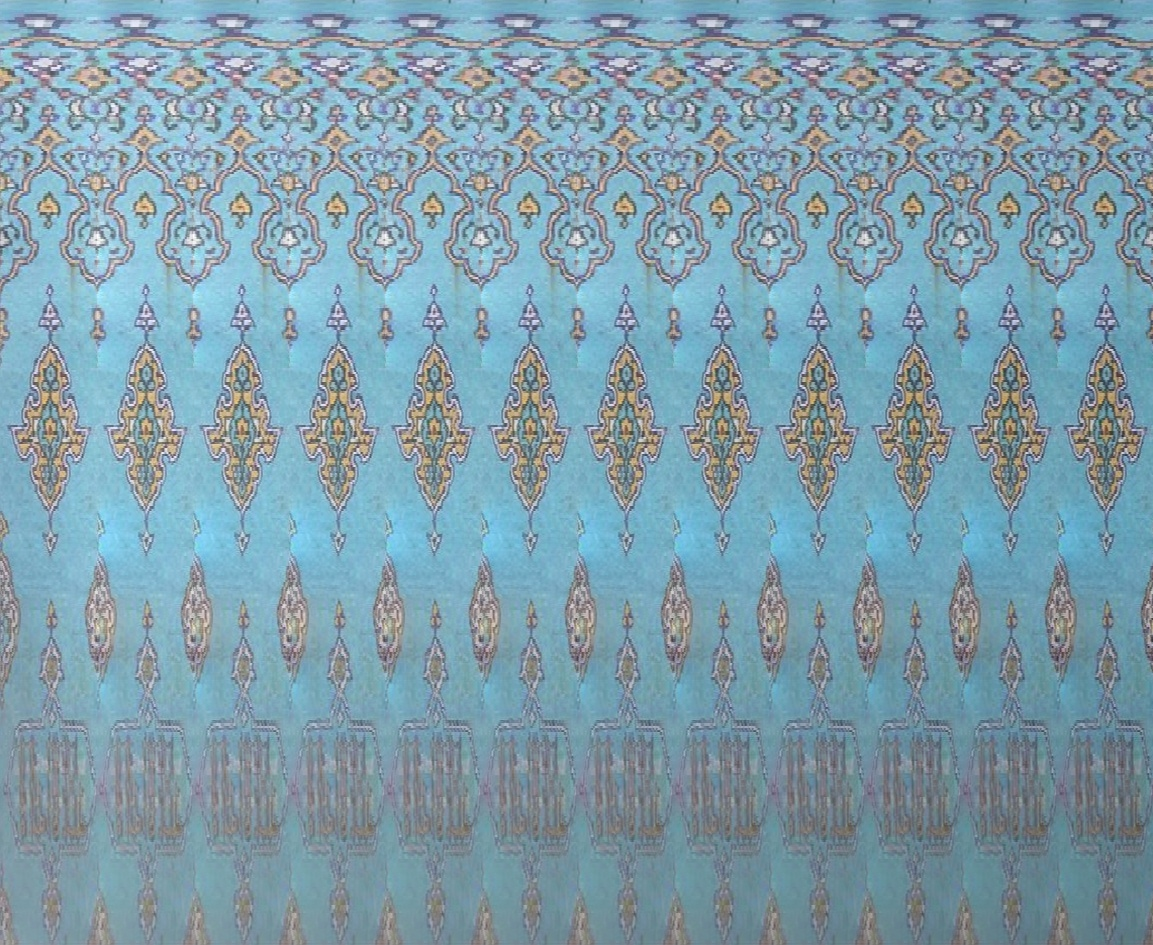
\includegraphics[height=5cm]{comparison-7}
	\caption{خروجی الگوریتم ادغام تصاویر با دوازده تکرار قطاع}
	\label{twelveRep}
\end{figure}

راه‌حل بعدی که پیاده‌سازی شد، اجرای الگوریتم به صورت قدم‌به‌قدم بوده است. در این روش، هر مرحله تنها دو تصویر با هم ادغام و ورودی‌های هر مرحله، با استفاده از خروجی قدم قبلی تولید می‌شوند. خروجی مرحله قبلی یک بار از سمت چپ با رنگ سفید گسترش می‌یابد و یک بار از سمت راست تا ورودی‌های مرحله فعلی را تشکیل دهد. این روش را با سه قدم اجرا کردیم: ابتدا با ورودی‌های تولید‌شده از قطاع اولیه، سپس با ورودی‌های تولید‌شده از دو قطاع به هم چسبیده و در انتها با استفاده از ورودی‌های تولید‌شده از چهار قطاع به هم چسبیده. نتایج این روش در شکل \ref{stepByStepRes} آورده شده است. نتایج برای قدم اول (\ref{stepByStepRes:f1}) و قدم دوم (\ref{stepByStepRes:f2}) مناسب هستند و به نظر مشکل انتشار رنگ سفید را هم ندارند. اما زمانی که به قدم آخر (\ref{stepByStepRes:f3}) می‌رسیم، مشاهده می‌شود به دلیل زیاد شدن مساحت رنگ سفید و زیاد شدن فاصله‌ی منطقه‌ی هم‌پوشانی از دو طرف تصویر، الگوریتم نتوانسته نتایج خوبی داشته باشد و علاوه بر به هم خوردن رنگ کلی بافت، خط اتصال میانی نیز به وضوح مشخص است.
\begin{figure}[h!]
	\centering
	\subfloat[]{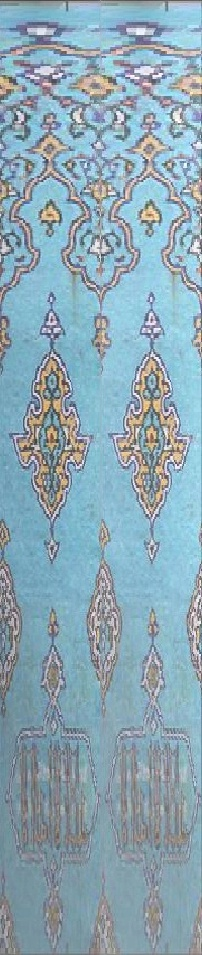
\includegraphics[height=5cm]{comparison-8}\label{stepByStepRes:f1}}
	\qquad
	\subfloat[]{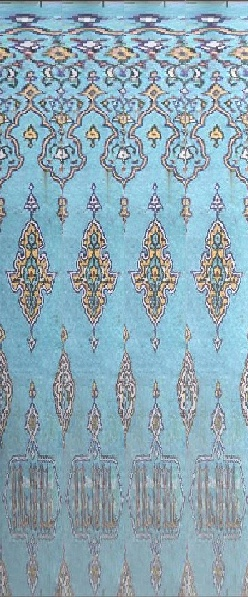
\includegraphics[height=5cm]{comparison-9}\label{stepByStepRes:f2}}
	\qquad
	\subfloat[]{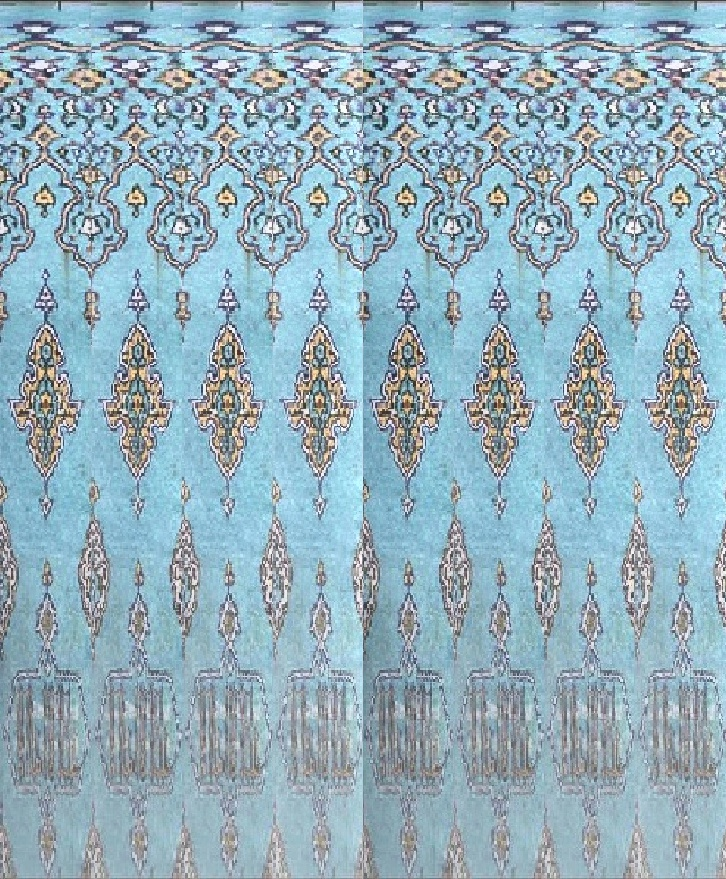
\includegraphics[height=5cm]{comparison-10}\label{stepByStepRes:f3}}
	\caption{اجرای الگوریتم ادغام تصاویر به صورت قدم‌به‌قدم}
	\label{stepByStepRes}
\end{figure}

\subsection{روش‌های یادگیری عمیق} \label{deepLearningRes}
در این قسمت با استفاده از دو روش مبتنی بر یادگیری عمیق  نتایج را تولید و تحلیل کردیم. با مشاهده نتایج، به نظر می‌رسد استفاده از یادگیری عمیق برای حفظ \gls{Structure} الگو مناسب نیست و نمی‌تواند بافت مناسب را تولید کند.

\subsubsection{تولید بافت با استفاده از شبکه عصبی پیچشی} \label{TexSynConvSec}
با استفاده از پژوهش 
\lr{Texture Synthesis Using Convolutional Neural Networks\cite{gatys2015texture}} 
نتایج این قسمت تولید شد. ورودی و خروجی الگوریتم در شکل \ref{TexSynConv} مشاهده می‌شود. در این شکل، تصویر \ref{TexSynConv:f1} ورودی الگوریتم و تصویر \ref{TexSynConv:f2} خروجی برای گسترش سه برابر عرض ورودی و طول برابر با ورودی است. خروجی به صورت کلی توانسته است رنگ بافت ورودی را حفظ کند و متوجه شده است رنگ قالب، رنگ پس‌زمینه است. مشکلی که در این روش مشاهده می‌شود، عدم حفظ ساختار الگو است که این باعث در‌هم‌ریختگی الگو در بافت نهایی شده است.
\begin{figure}[h!]
	\centering
	\subfloat[]{
\includegraphics[height=5cm]{comparison-11}\label{TexSynConv:f1}}
	\qquad
	\subfloat[]{
\includegraphics[height=5cm]{comparison-12}\label{TexSynConv:f2}}
	\caption{اجرای الگوریتم تولید بافت با استفاده از شبکه عصبی پیچشی}
	\label{TexSynConv}
\end{figure}

\subsubsection{بافت‌های بهینه}
این قسمت نتایج تولید شده با استفاده از الگوریتم 
\lr{Optimal Textures\cite{risser2020optimal}}
آمده است. این الگوریتم دو هدف متفاوت را می‌تواند اجرا کند. هدف اول مانند \ref{TexSynConvSec}، برای گسترش تصاویر است. در این هدف، ما برای تنظیمات الگوریتم، عرض خروجی را چهار برابر و طول آن را برابر با ورودی مشخص کردیم. ورودی و خروجی الگوریتم برای این هدف در شکل \ref{OpTex1} آمده است که تصویر \ref{OpTex1:f1} ورودی الگوریتم و تصویر \ref{OpTex1:f2} خروجی تولید‌شده را نمایش می‌دهد. خروجی این قسمت ویژگی‌های مشابه با \ref{TexSynConvSec} دارد که با توجه به عدم تمرکز بر روی مشکل حفظ ساختار الگو‌ها در این پژوهش نسبت به پژوهش قبلی، این نتایج آن چنان دور از انتظار نبود.
\begin{figure}[h!]
	\centering
	\subfloat[]{
\includegraphics[height=5cm]{comparison-13}\label{OpTex1:f1}}
	\qquad
	\subfloat[]{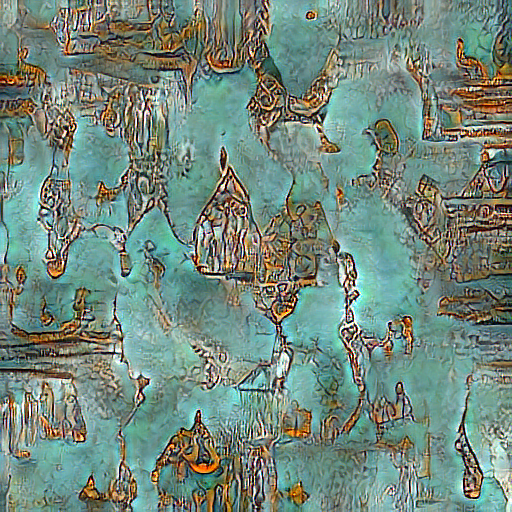
\includegraphics[height=5cm]{comparison-14}\label{OpTex1:f2}}
	\caption{اجرای الگوریتم بافت‌های بهینه با هدف گسترش}
	\label{OpTex1}
\end{figure}

هدف دیگری که پژوهش بافت‌های بهینه ارائه می‌دهد، ادغام تصاویر ‌(مانند \ref{imageFusion}) است. ورودی و خروجی اجرای الگوریتم برای این هدف در شکل \ref{OpTex2} آمده است. تصاویر \ref{OpTex2:f1} و \ref{OpTex2:f2} ورودی تولید شده برای این هدف هستند و تصویر \ref{OpTex2:f3} خروجی الگوریتم را نمایش می‌دهد. با استفاده از این هدف، نتایج باز هم مناسب نیستند و به رنگ سفید وزن بیشتری نسبت به الگوی ورودی داده شده است.
\begin{figure}[h!]
	\centering
	\subfloat[]{\fbox{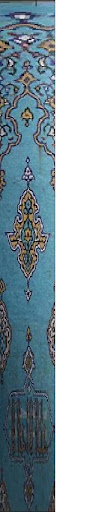
\includegraphics[height=5cm]{comparison-15}\label{OpTex2:f1}}}
	\qquad
	\subfloat[]{\fbox{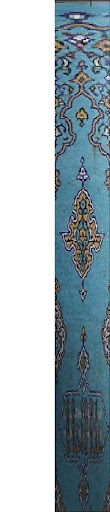
\includegraphics[height=5cm]{comparison-16}\label{OpTex2:f2}}}
	\qquad
	\subfloat[]{\fbox{
\includegraphics[height=5cm]{comparison-17}\label{OpTex2:f3}}}
	\caption{اجرای الگوریتم بافت‌های بهینه برای ادغام تصاویر}
	\label{OpTex2}
\end{figure}

\subsection{روش‌های مبتنی بر وصله} \label{patchBasedRes}
در این قسمت نتایج را با یک پیاده‌سازی روش‌های مبتنی بر وصله\cite{patchBaseGit} که با استفاده از پژوهش‌های 
\lr{Image Quilting} 
و
\lr{Real-Time Texture Synthesis by Patch-Based Sampling\cite{patchBasedSampling}} 
نوشته شده است، تولید کردیم. در ابتدا الگوریتم را با استفاده از یک قطاع به عنوان ورودی، اجرا کردیم. ورودی (قسمت سمت راست تصویر) و خروجی (قسمت سمت چپ تصویر) در شکل \ref{patch1} نمایش داده شده است. گسترش انتخاب شده برای طول و عرض دو برابری خروجی نسبت به ورودی بوده‌است. وصله‌های انتخاب شده برای تولید خروجی ساختار مناسبی ندارند و الگوریتم با استفاده از معیار فاصله خود نتوانسته وصله‌های مناسبی را انتخاب کند.
\begin{figure}[h!]
	\centering
	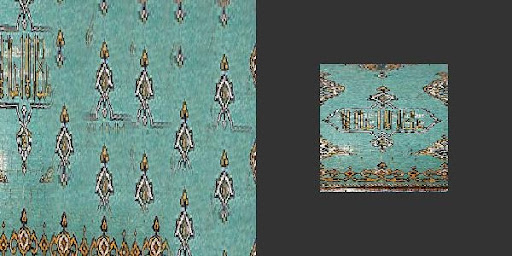
\includegraphics[height=5cm]{comparison-18}
	\caption{ورودی و خروجی روش مبتنی بر وصله با یک قطاع}
	\label{patch1}
\end{figure}
\newline
برای اینکه امکان تولید نتایج مناسب را بالا ببریم، از خروجی اتصال چهار قطاع، که با استفاده از \ref{imageFusion} تولید شده است، به عنوان ورودی برای الگوریتم انتخاب کردیم. ورودی و خروجی در شکل \ref{patch2} آمده است. با استفاده از چهار قطاع، الگوریتم توانسته با استفاده از معیار فاصله خود، وصله‌های بهتری برای خروجی پیدا کند، اما در بعضی مناطق باز هم دچار اشتباه شده و خروجی ساختار کامل را رعایت نکرده است. به نظر می‌رسد تضمین کاملی برای انتخاب وصله‌های مناسب توسط الگوریتم وجود ندارد. مشکل دیگری که پر این الگوریتم وجود دارد، انتخاب وصله‌ها به صورت مربعی است. تلاش شد با تغییر کد کاری کرد که نیازی به انتخاب فرمت مربعی برای خروجی و وصله‌ها نباشد، اما به نتیجه نرسید و اندازه‌ها با یکدیگر هماهنگ نشدند. دلیل اصلی این اتفاق تفاوت ترتیب طول و عرض در ماتریس تصاویر 
\lr{OpenCV} 
و 
 \lr{NumPy}
 بود که به علت مربعی بودن پیاده‌سازی اصلی، در خیلی از قسمت‌های کد این اشتباه رخ داده و امکان تغییر نبود.
\begin{figure}[h!]
	\centering
	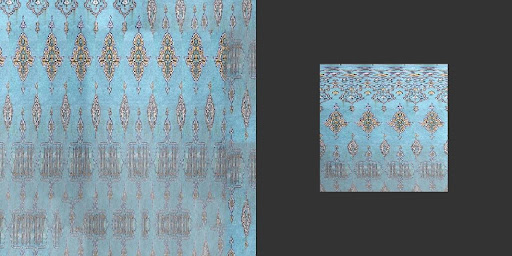
\includegraphics[height=5cm]{comparison-19}
	\caption{ورودی و خروجی روش مبتنی بر وصله با چهار قطاع}
	\label{patch2}
\end{figure}

\subsection{آینده کردن تصویر} \label{mirroringRes}
در این قسمت با استفاده از روش آینه‌کردن تلاش می‌شود تصویر از لحاظ رنگی و شدت نوری هموار شود. در صورتی که قطاع در نظر گرفته‌شده حاوی طرح متقارن باشد، استفاده از این تکنیک هم در فضای RGB و هم در فضای LUV می‌تواند هموار کردن را به صورت مناسبی انجام دهد. مشکل اصلی این الگوریتم در شکل \ref{mirroring} نمایش داده شده است. این خروجی برای قطاع \ref{compInputs:f1} تولید شده است که حاوی قسمت متنی بوده است. خروجی این روش، با اینکه از لحاظ نوری و رنگی هموار است و در مکان‌های اتصال قطاع‌ها خطی مشاهده نمی‌شود، قسمت متنی قطاع را به هم ریخته و ساختار را خراب کرده است.
\begin{figure}[h!]
	\centering
	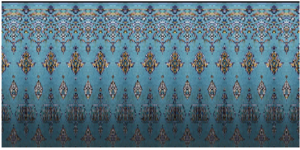
\includegraphics[height=5cm]{comparison-20}
	\caption{خروجی استفاده از روش آینه‌کردن در قطاع حاوی متن}
	\label{mirroring}
\end{figure}

\subsection{الگوریتم ارائه‌شده} \label{ourAlgCompRes}
در این قسمت نتایج تولید شده با استفاده از روش ما با استفاده از ورودی‌های \ref{compInputs} تولید شده است. در شکل \ref{compOurs1} بافت تولید شده برای ورودی قطاع \ref{compInputs:f1} آمده است. همانطور که در تصویر مشخص است، الگوریتم ما توانسته به صورت مناسب مرز‌های بین قطاع‌ها را حذف کند و بافت همواری را تولید کند. در خروجی مشخص است که مشکل انتشار رنگ سفید (مشکل مشاهده شده در بخش \ref{imageFusion}) حل شده و الگوریتم توانسته ساختار ورودی را، برخلاف روش‌های یادگیری عمیق اجرا‌شده در بخش \ref{deepLearningRes} و \ref{patchBasedRes}، حفظ کند. نسبت به روش آینه‌کردن تصاویر (بخش \ref{mirroringRes})، الگوریتم ما در هموار کردن با آن برابری می‌کند، اما مشکل در هم ریختگی قسمت متنی را ندارد.

 تنها مشکلی که در این خروجی مشاهده می‌شود، در بالای بافت تولید شده است که به صورت کامل خط بین قطاع‌ها برطرف نشده است. دلیل وجود این مشکل تفاوت زیاد نوری این بخش از قطاع در دو طرف تصویر است که به علت ساختار هندسه‌ی شیء انتخاب‌شده برای مدل‌سازی بوجود آمده. مدل انتخاب شده یک گنبد بوده که به علت هندسه‌ی آن، بخش بالای تصویر در اصل مساحت بسیار کمتری را نسبت به قسمت میانی تصویر بر روی گنبد شامل می‌شود. البته با توجه به هندسه‌ی مدل سه‌بعدی که باید بافت بر روی آن نگاشت شود، این مشکل به علت فشرده شدن بخش بالای تصویر، دیده نمی‌شود.
\begin{figure}[h!]
	\centering
	
\includegraphics[height=5cm]{comparison-21}
	\caption{بافت تولید شده از الگوریتم ارائه‌شده برای ورودی \ref{compInputs:f1}}
	\label{compOurs1}
\end{figure}

در شکل \ref{compOurs2} بافت تولید شده برای قطاع \ref{compInputs:f2} نمایش داده شده است. همانطور که مشخص است، این بافت مشکلات خروجی‌های بخش‌های قبلی را ندارد و از لحاظ رنگی و نوری هموار می‌باشد. ایرادی که امکان دارد از این بافت گرفته شود، وجود انعکاس نور در وسط و پایین تصویر است که  همراه با قطاع بوده و در هر تکرار قطاع دیده می‌شود. با توجه به اینکه در روش ارائه‌شده، ما تمرکز خود را بر روی نواحی حاشیه قطاع قرار داده‌ایم، وجود اعوجاج در میانه‌ی قطاع برای ما اهمیتی ندارد و آن را بررسی نمی‌کنیم. در نتیجه انتخاب قطاع مناسب برای تولید بافت بدون مشکل در الگوریتم ما مهم است.
\begin{figure}[h!]
	\centering
	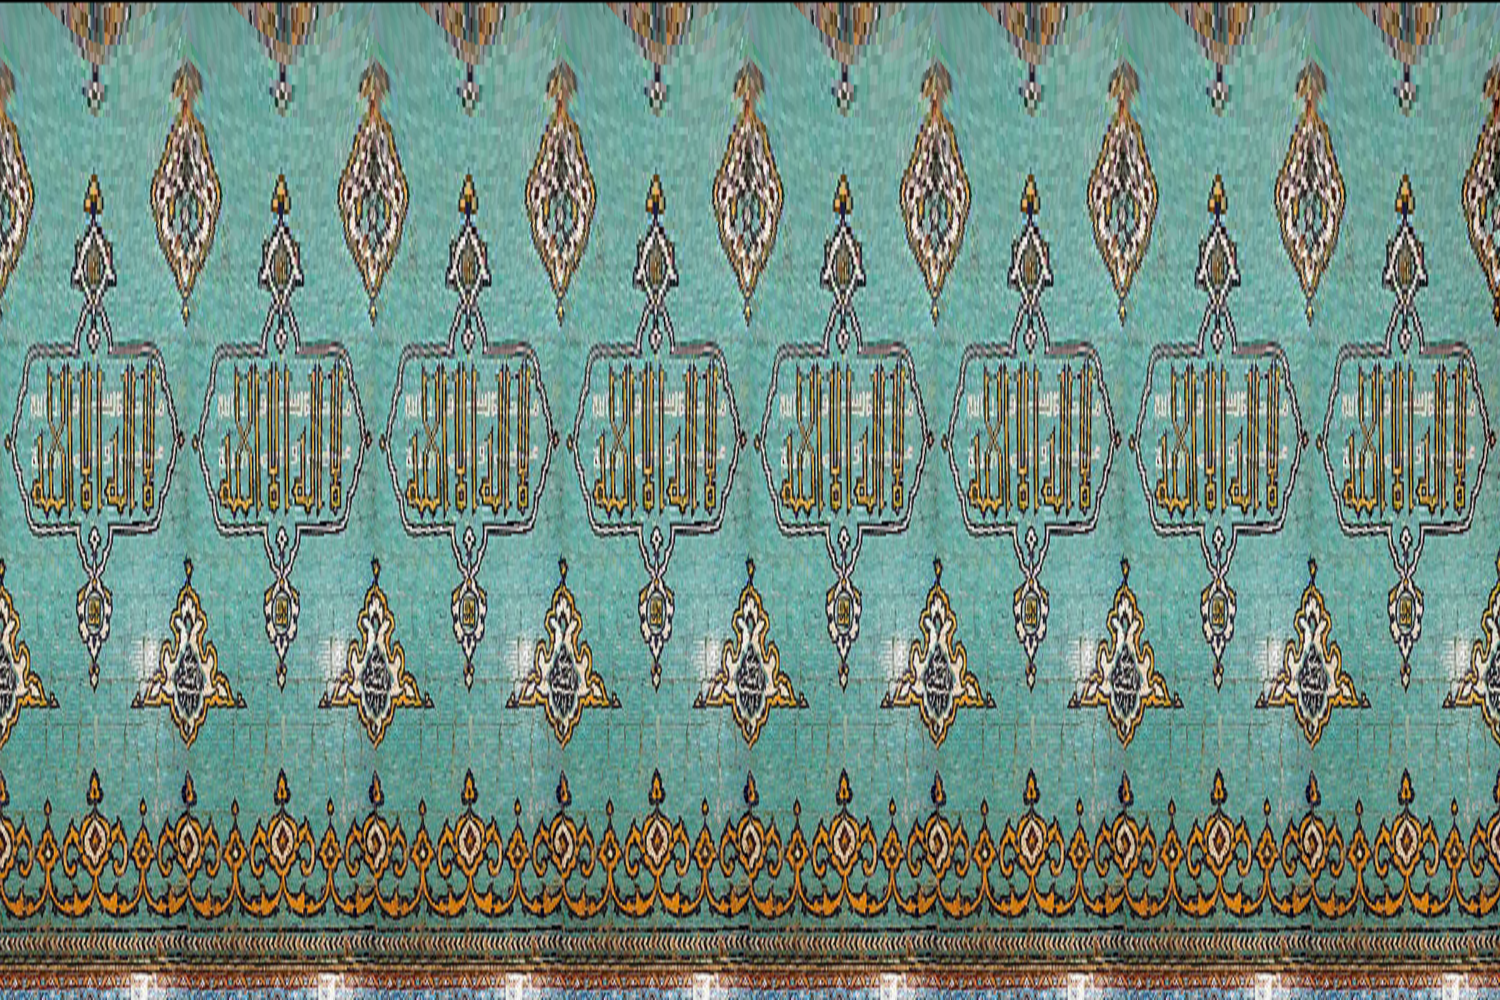
\includegraphics[height=5cm]{comparison-22}
	\caption{بافت تولید شده از الگوریتم ارائه‌شده برای ورودی \ref{compInputs:f2}}
	\label{compOurs2}
\end{figure}

\section{بازسازی سه‌بعدی با استفاده از یک تصویر}
در این قسمت نتایج استفاده از روش ارائه‌شده در مسئله‌ی تولید بافت برای بازسازی سه‌بعدی از یک تصویر را نمایش داده‌ایم. برای مدل‌سازی هندسه و استخراج بافت رویی شیء، از الگوریتم رویه دورانی استفاده شده است. روش استفاده شده در آن الگوریتم، به صورت پیش‌فرض، تکرار الگوی رویی برای قسمت پشتی شیء بوده که ما این روش را برای بعضی از اشیاء اجرا و نتایج آن را با نتایج تولید‌شده با استفاده از روش خودمان مقایسه کردیم.

در ابتدا برای تکمیل کردن نتایج بخش قبل، در شکل \ref{res1In} تصویر اصلی شیء که قطاع \ref{compInputs:f1} از آن استخراج شده بود، در کنار خود قطاع آورده شده است. همانطور که گفته‌شد، هندسه‌ی مدل به صورت جداگانه از تصویر \ref{res1In:f1} استخراج می‌شود و تمرکز ما تنها بر روی تولید بافت بوده است.
\begin{figure}[h!]
	\centering
	\subfloat[تصویر اصلی شیء]{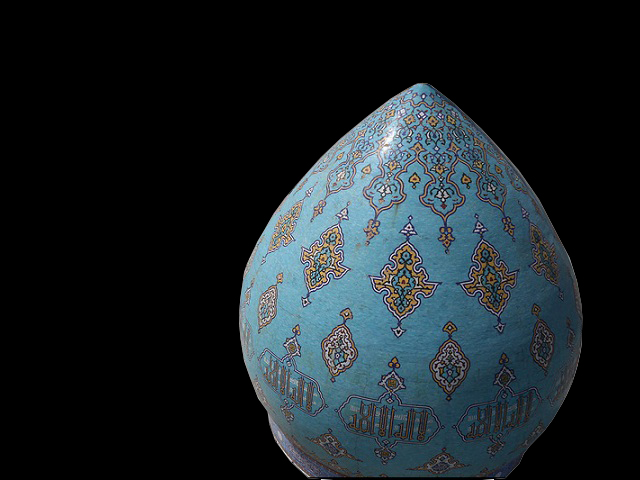
\includegraphics[height=4cm]{ourRes-1}\label{res1In:f1}}
	\qquad
	\subfloat[قطاع استخراج‌شده]{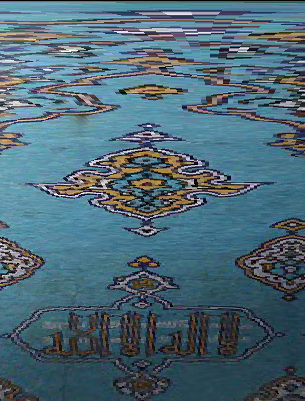
\includegraphics[height=4cm]{ourRes-2}\label{res1In:f2}}
	\caption{ورودی‌های اول الگوریتم ارائه‌شده}
	\label{res1In}
\end{figure}
\newline
بافت تولید‌شده با استفاده از روش ارائه‌شده در شکل \ref{res1Out} آورده شده است که ویژگی‌های آن در بخش \ref{ourAlgCompRes} شرح داده شد. این خروجی با دوازده تکرار قطاع مشخص‌شده در \ref{res1In:f2} تولید شده است.
\begin{figure}[h!]
	\centering
	
\includegraphics[height=5cm]{ourRes-3}
	\caption{بافت تولید شده از الگوریتم ارائه‌شده برای ورودی اول}
	\label{res1Out}
\end{figure}
\newline
خروجی تولید‌شده پس از نگاشت بافت خروجی از روش ما بر روی هندسه‌ی تولید‌شده، در شکل \ref{res1_3DOut} آورده شده است. بازسازی صورت گرفته از لحاظ ویژگی‌های ظاهری مناسب می‌باشد. هندسه سه‌بعدی استخراج‌شده ارتفاع کامل گنبد را شامل نشده اما بافت استخراج شده نیز همین ویژگی را دارد. تنها مشکلی که به ظاهر وجود دارد، یکسان نبودن تعداد تکرار قطاع در بافت تولید‌شده نسبت به تصویر جسم است، که این تعداد تکرار از الگوریتم رویه دورانی استخراج شده بود. البته این مشکل را به راحتی می‌توان با انتخاب تعداد مناسب تکرار به عنوان ورودی برای الگوریتم ارائه شده حل کرد.
\begin{figure}[h!]
	\centering
	\subfloat[]{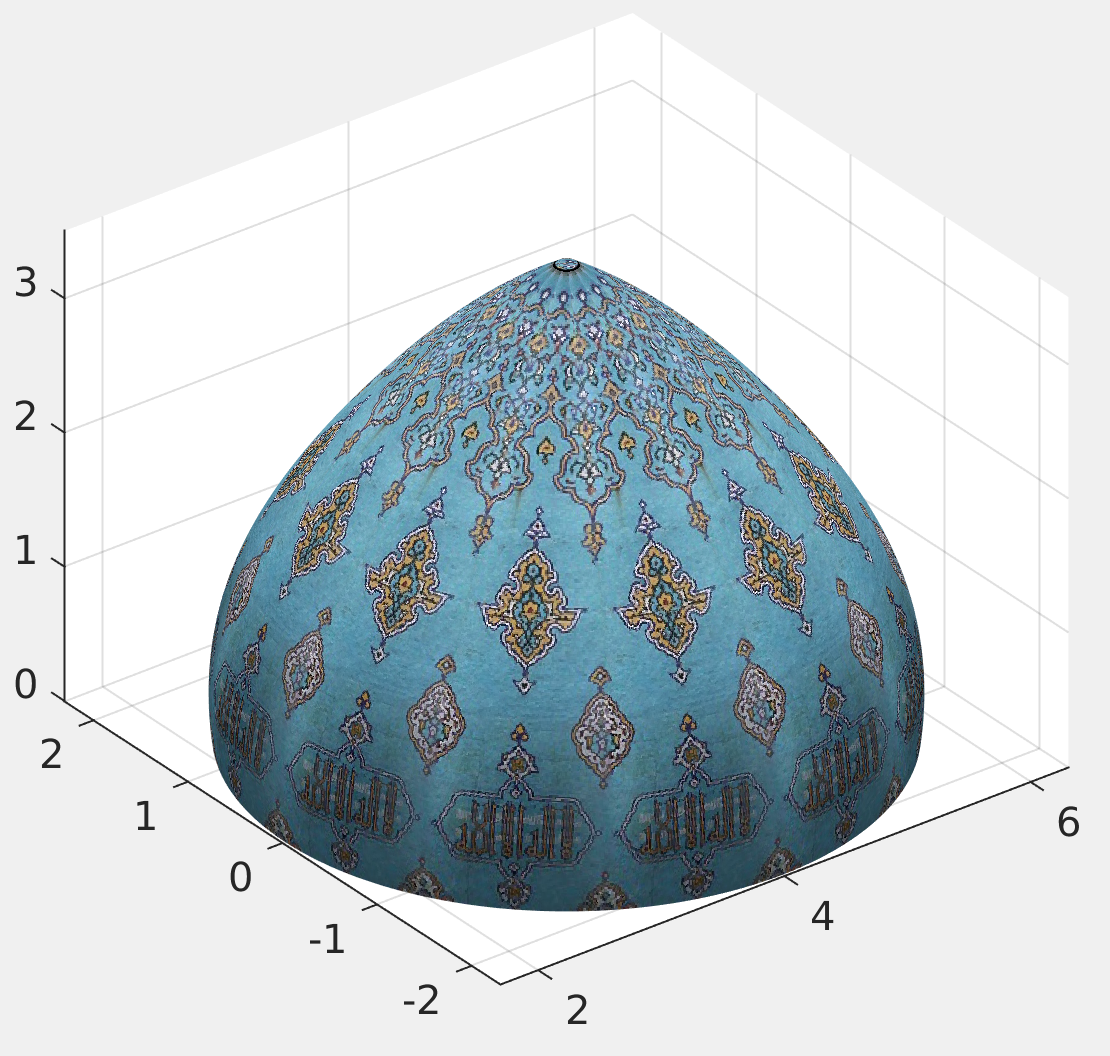
\includegraphics[height=4cm]{ourRes-4}\label{res1_3DOut:f1}}
	\qquad
	\subfloat[]{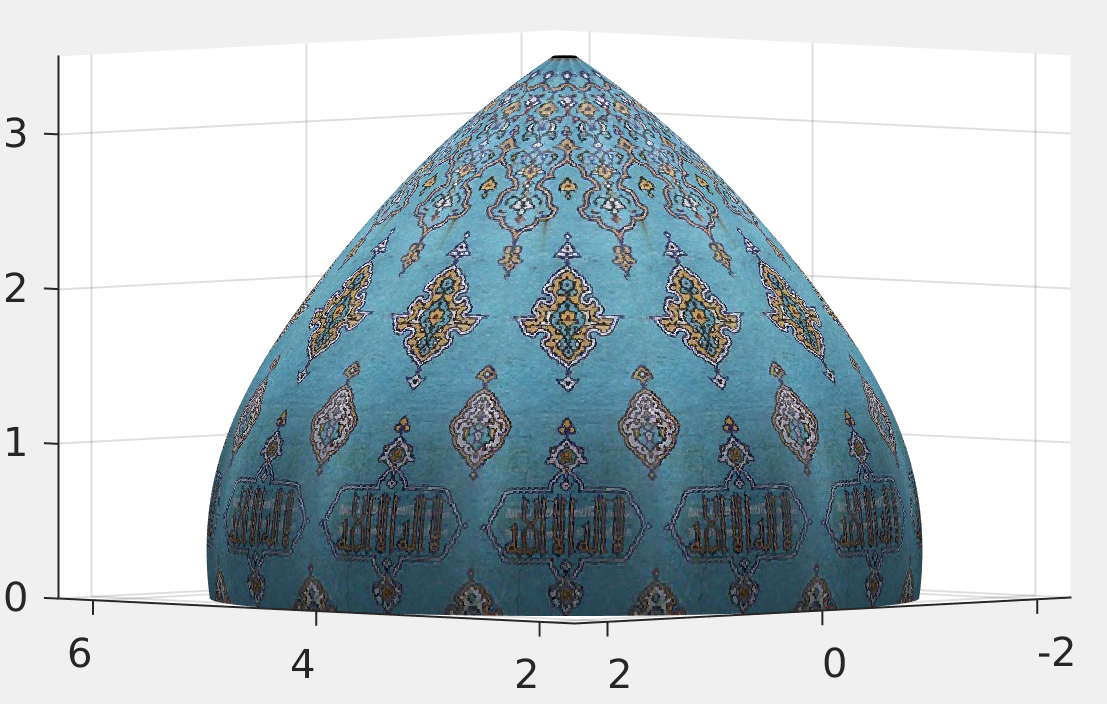
\includegraphics[height=4cm]{ourRes-5}\label{res1_3DOut:f2}}
	\caption{مدل سه‌بعدی بازسازی شده اول}
	\label{res1_3DOut}
\end{figure}

ورودی بعدی انتخاب‌شده در شکل \ref{res2In} آمده است که همان قطاع \ref{compInputs:f2} به همراه تصویر اصلی شیء است که قطاع از آن استخراج شده بود.
\begin{figure}[h!]
	\centering
	\subfloat[تصویر اصلی شیء]{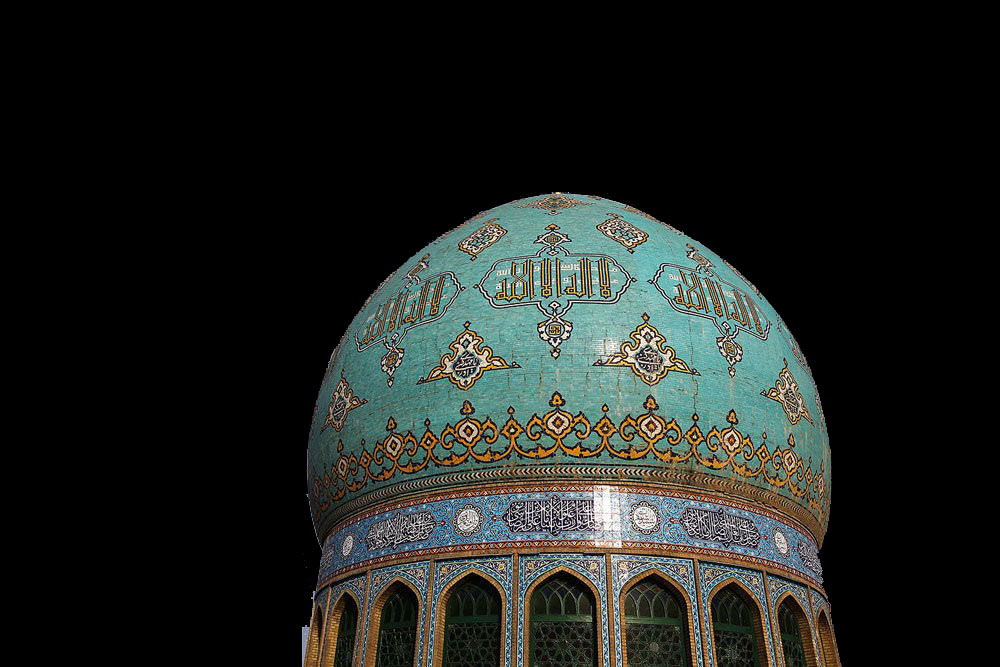
\includegraphics[height=4cm]{ourRes-6}\label{res2In:f1}}
	\qquad
	\subfloat[قطاع استخراج‌شده]{
\includegraphics[height=4cm]{ourRes-7}\label{res2In:f2}}
	\caption{ورودی‌های دوم الگوریتم ارائه‌شده}
	\label{res2In}
\end{figure}
\newline
بافت تولید‌شده در شکل \ref{res2Out} آمده است که در بخش \ref{ourAlgCompRes} ویژگی‌های این بافت را نیز شرح دادیم. این بافت با هشت تکرار قطاع تولید‌شده است.
\begin{figure}[h!]
	\centering
	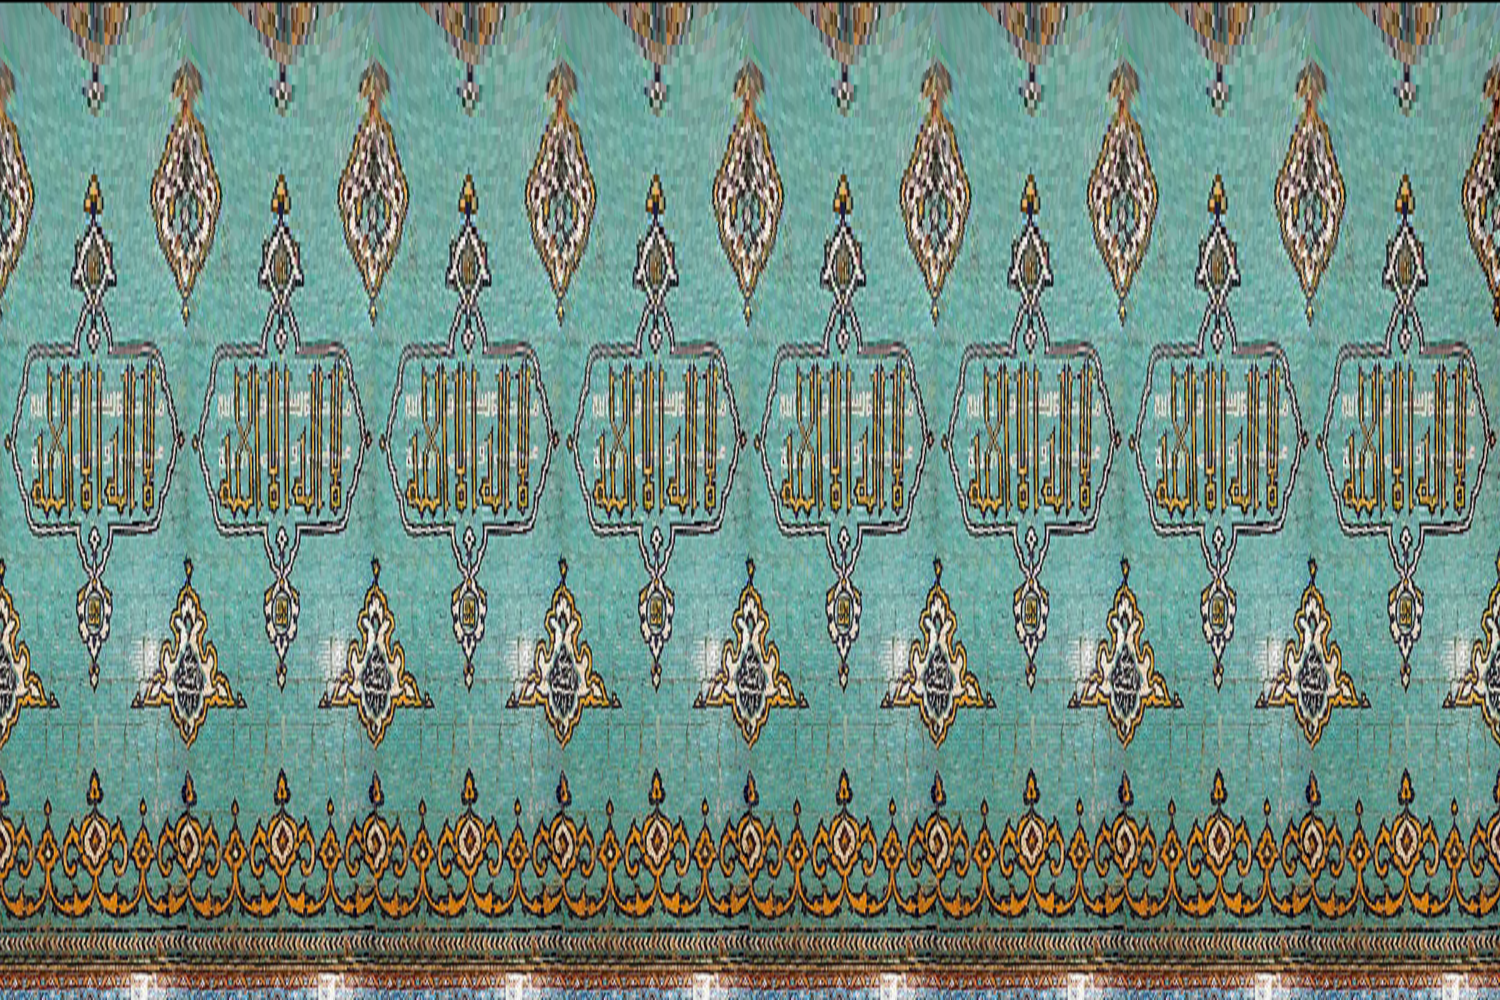
\includegraphics[height=5cm]{ourRes-8}
	\caption{بافت تولید شده از الگوریتم ارائه‌شده برای ورودی دوم}
	\label{res2Out}
\end{figure}

مدل نهایی بازسازی شده در شکل \ref{res2_3DOut} آمده است. برای این شیء هم مدل سه‌بعدی بازسازی شده کامل نیست اما الگوی متناسب استخراج شده بوده و بافت نهایی تولید‌شده هموار و مناسب است. در این شیء تکرار قطاع مناسب است و مدل سه‌بعدی نهایی شباهت مطلوبی با شیء اصلی در تصویر ورودی دارد. تنها مشکلی که در بافت مشاهده می‌شود، قسمت بالایی بافت است که به علت زاویه دوربین، از ناحیه‌ای استخراج شده که بعد از گسترش به الگوی مستطیلی، کشیدگی زیادی داشته و اندکی محو شده است. اما این مشکل به علت زاویه دوربین در تصویر ورودی بوده و روش ارائه‌شده‌ی ما بر روی این موضوع تمرکزی ندارد.
\begin{figure}[h!]
	\centering
	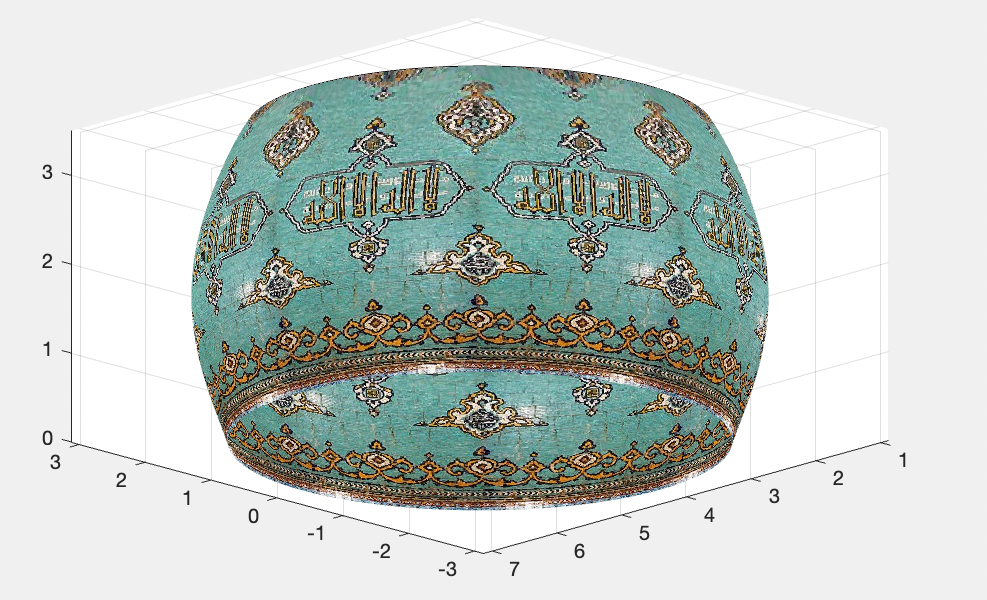
\includegraphics[height=5cm]{ourRes-9}
	\caption{مدل سه‌بعدی بازسازی شده دوم}
	\label{res2_3DOut}
\end{figure}

ورودی سوم در شکل \ref{res3In} آمده است. شیء مورد نظر (تصویر \ref{res3In:f1}) یک کوزه است که قطاع آن سه بار تکرار شده است. همانطور که از تصویر مشخص است، در صورتی که الگوی رویی شیء را برای قسمت پشت آن تکرار کنیم، در جلو و پشت شیء یک تکرار کامل قطاع داریم و در دو طرف شی هر کدام یک قسمت کوچک از قطاع وجود داردک ه تشکیل یک قطاع کامل را نمی‌دهند. مدل سه‌بعدی بازسازی‌شده با استفاده از این روش در شکل \ref{res3_bad} آمده است که این مشکل در تکرار ساده نشان می‌دهد. در تصویر \ref{res3In:f2} قطاع نهایی پس از استخراج الگو و برش آن آمده است. مشکلی که در قطاع دیده می‌شود، عمودی نبودن خط‌های دهانه‌ی کوزه است. این مشکل به علت استخراج نامناسب الگوی رویی  به دلیل دقیق نشدن هندسه‌ی مدل بر روی تصویر، پیش آمده است. با توجه به اینکه این مرحله توسط الگوریتم ارائه‌شده انجام نمی‌شود، برای بهبود این قسمت کاری انجام نشده است.
\begin{figure}[h!]
	\centering
	\subfloat[تصویر اصلی شیء]{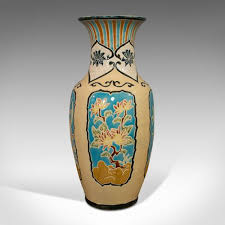
\includegraphics[height=4cm]{ourRes-11}\label{res3In:f1}}
	\qquad
	\subfloat[قطاع استخراج‌شده]{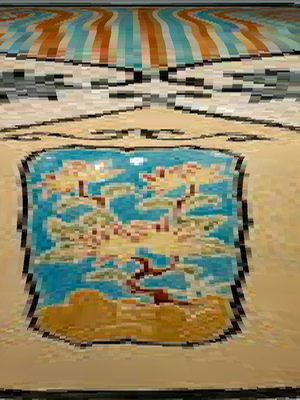
\includegraphics[height=4cm]{ourRes-12}\label{res3In:f2}}
	\caption{ورودی‌های سوم الگوریتم ارائه‌شده}
	\label{res3In}
\end{figure}
\begin{figure}[h!]
	\centering
	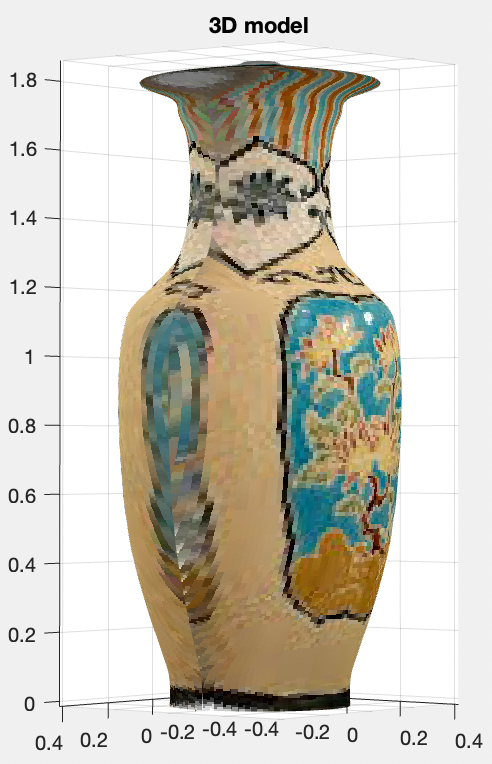
\includegraphics[height=5cm]{ourRes-10}
	\caption{مدل سه‌بعدی بازسازی‌شده برای ورودی سوم با استفاده از تکرار ساده طرح رویی برای پشت}
	\label{res3_bad}
\end{figure}

مطابق شکل \ref{res3Out}، بافت نهایی از قطاع با انجام سه تکرار تولید شده است. قطاع نهایی (\ref{res3in:f2}) با استفاده از روش رفع واپیچش، هموار‌تر شده تا در دو طرف قطاع مشکلی برای اتصال مناسب الگو‌ها به هم نداشته باشیم. بافت نهایی تولید شده به علت کم بودن کیفیت تصویر و نامنظم بودن الگوی کوزه، اندکی از لحاظ ظاهری مشکل دارد. البته این مشکل بعد از نگاشت بافت به هندسه‌ی سه‌بعدی کم‌رنگ‌تر شده است. در بافت نهایی نیز مشکل خطوط عمودی بالای الگو دیده می‌شود اما الگوریتم تلاش کرده این قسمت را هم هموار کند که مشاهده می‌شود خط محکمی در این قسمت نیز دیده نمی‌شود.
\begin{figure}[h!]
	\centering
	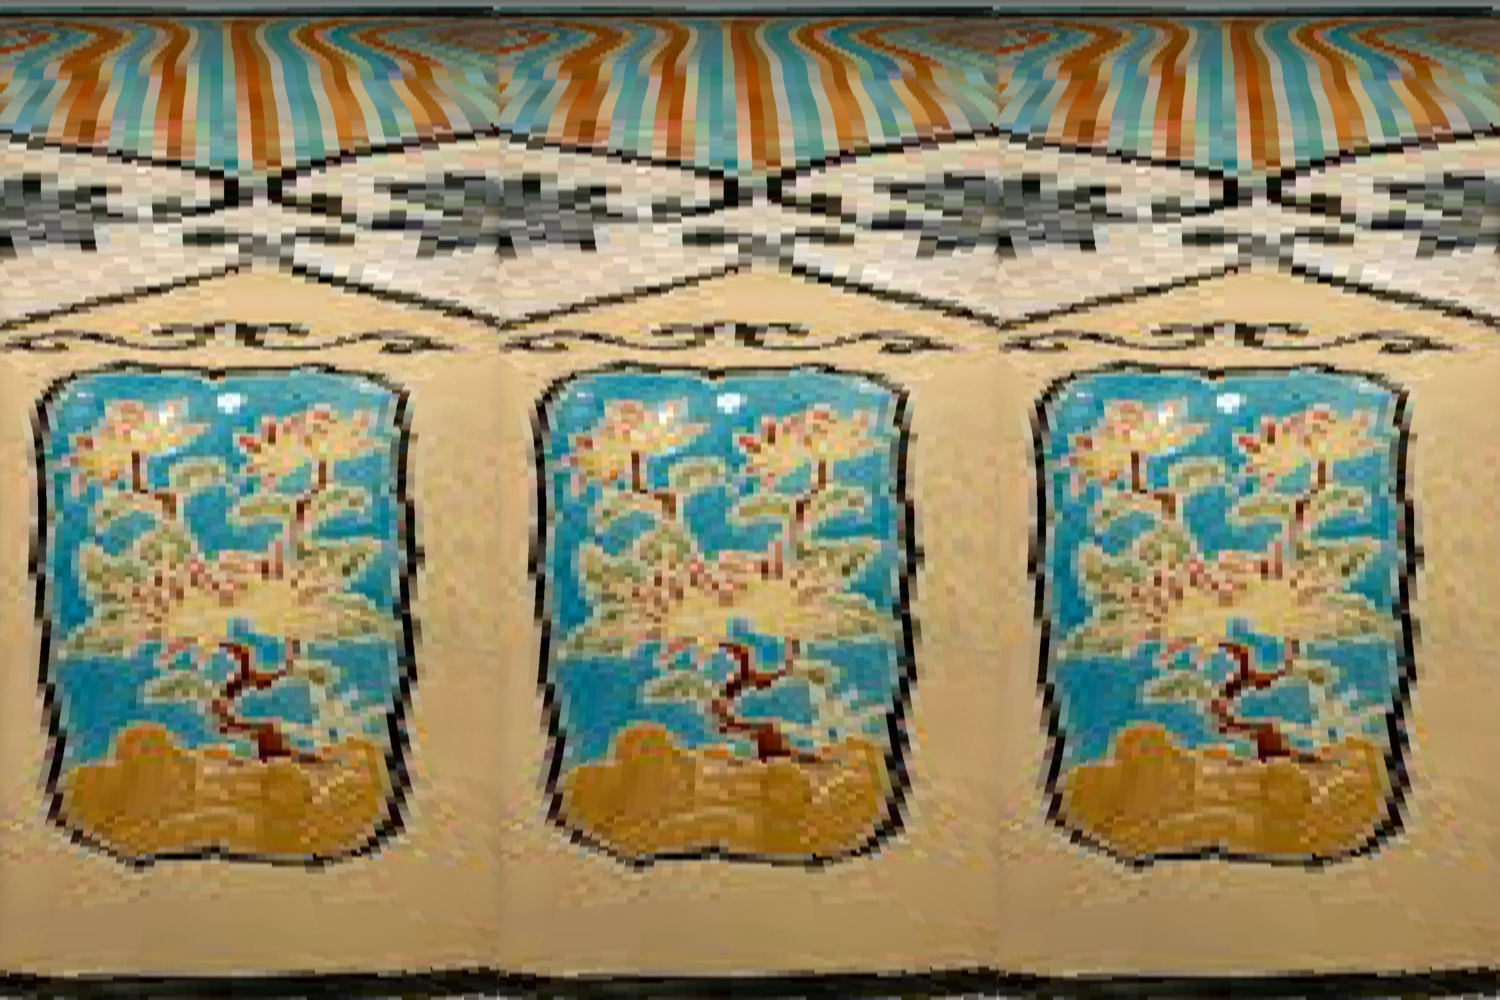
\includegraphics[height=5cm]{ourRes-13}
	\caption{بافت تولید شده از الگوریتم ارائه‌شده برای ورودی سوم}
	\label{res3Out}
\end{figure}

در شکل \ref{res3_3DOut} مدل سه‌بعدی نهایی بعد از نگاشت بافت تولید‌شده بر روی هندسه‌ی مدل آمده است. در مقایسه با شکل \ref{res3_bad}، مشاهده می‌شود روش ارائه‌شده، نتیجه‌ی مطلوب‌تری برای شیء حاوی تکرار فرد در الگوی خود، نسبت به روش استفاده از الگوی رویی برای الگوی پشتی داشته که این موضوع جزو برتری‌های روش ما نسبت به دیگر روش‌ها است.
\begin{figure}[h!]
	\centering
	\subfloat[]{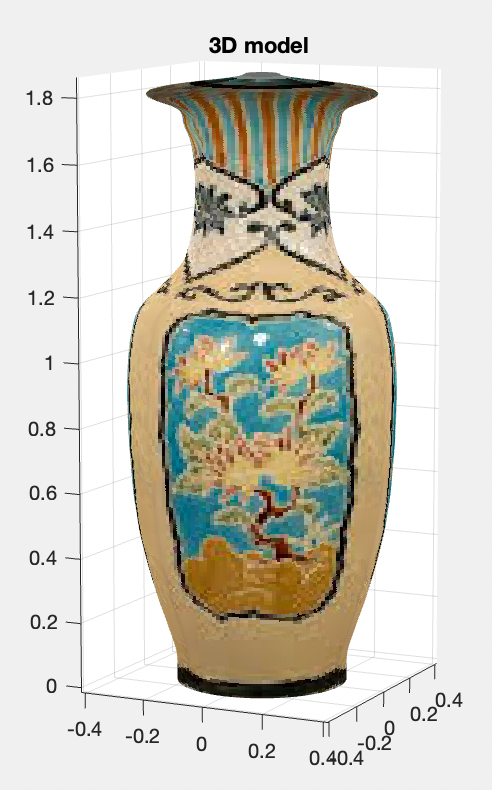
\includegraphics[height=5cm]{ourRes-14}\label{res3_3DOut:f1}}
	\qquad
	\subfloat[]{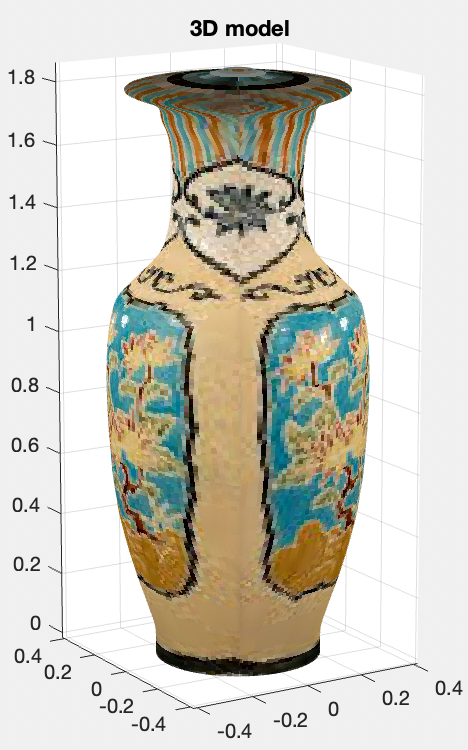
\includegraphics[height=5cm]{ourRes-15}\label{res3_3DOut:f2}}
	\caption{مدل سه‌بعدی بازسازی شده سوم}
	\label{res3_3DOut}
\end{figure}
\newline
ورودی بعدی اندکی با موارد قبلی تفاوت دارد. این ورودی (تصویر \ref{res4In:f1}) یک کوزه با تعداد تکرار‌های زیاد در الگوی تکرار شونده خود است. قطاع انتخاب‌شده در تصویر \ref{res4In:f2} آمده است. این قطاع نسبت به قطاع‌های قبلی باریک‌تر است اما برای بهتر دیده‌شدن، نسبت طول به عرض آن تغییر داده ‌شده است.
\begin{figure}[h!]
	\centering
	\subfloat[تصویر اصلی شیء]{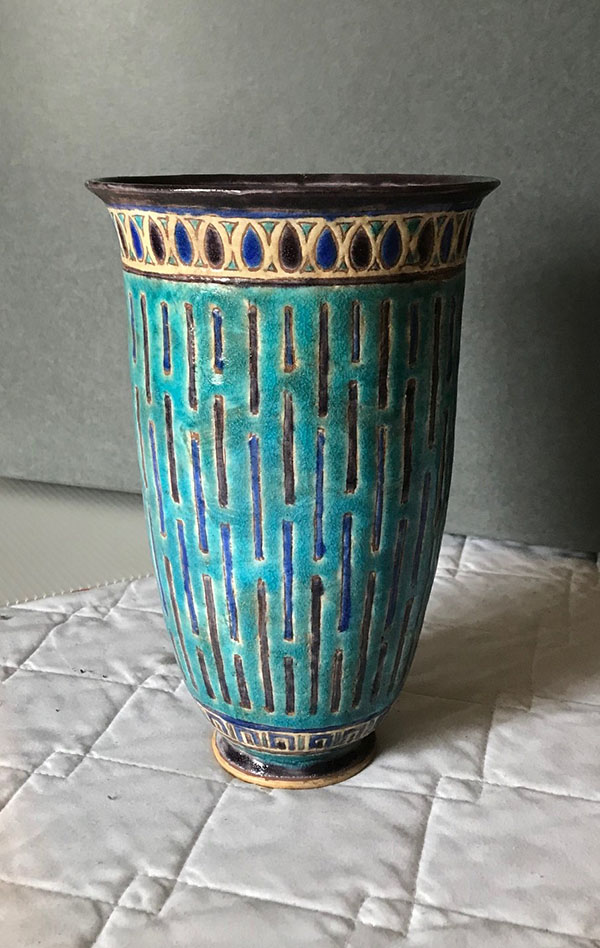
\includegraphics[height=4cm]{ourRes-16}\label{res4In:f1}}
	\qquad
	\subfloat[قطاع استخراج‌شده]{
\includegraphics[height=4cm]{ourRes-17}\label{res4In:f2}}
	\caption{ورودی‌های چهارم الگوریتم ارائه‌شده}
	\label{res4In}
\end{figure}
\newline
بافت نهایی تولید‌شده برای این قطاع با شانزده تکرار در شکل \ref{res4Out} آمده است. این بافت به نظر هموار است و هم قسمت بالایی آن و هم قسمت پایینی آن به صورت مناسبی تکرار شده و به یکدیگر چسبانده شده است.
\begin{figure}[h!]
	\centering
	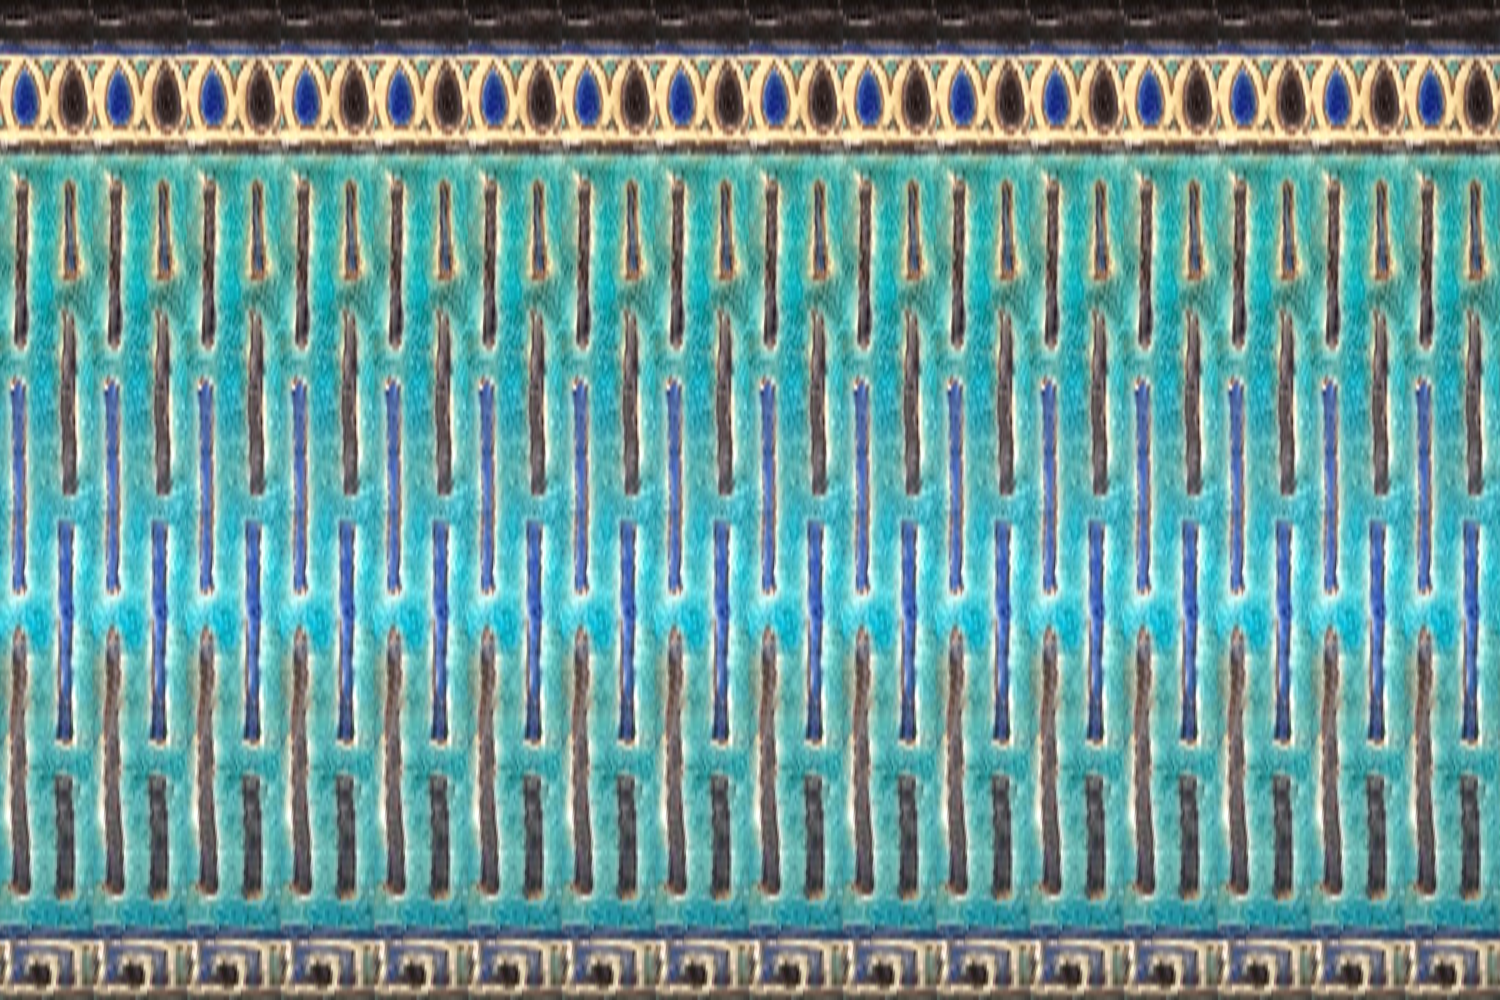
\includegraphics[height=5cm]{ourRes-18}
	\caption{بافت تولید شده از الگوریتم ارائه‌شده برای ورودی چهارم}
	\label{res4Out}
\end{figure}

در شکل \ref{res4_3DOut} مدل سه‌بعدی نهایی تولید‌شده مشخص است. این مدل از لحاظ ظاهری بسیار مشابه به شیء اصلی است و هم هندسه و هم بافت نهایی تولید شده مناسب بوده است.
\begin{figure}[h!]
	\centering
	\subfloat[]{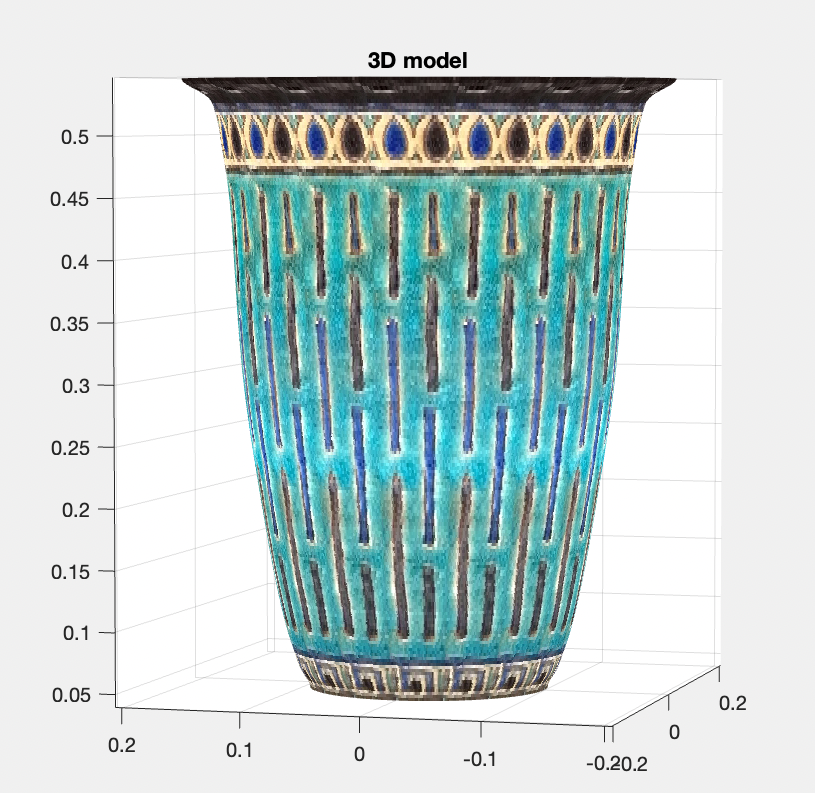
\includegraphics[height=5cm]{ourRes-19}\label{res4_3DOut:f1}}
	\qquad
	\subfloat[]{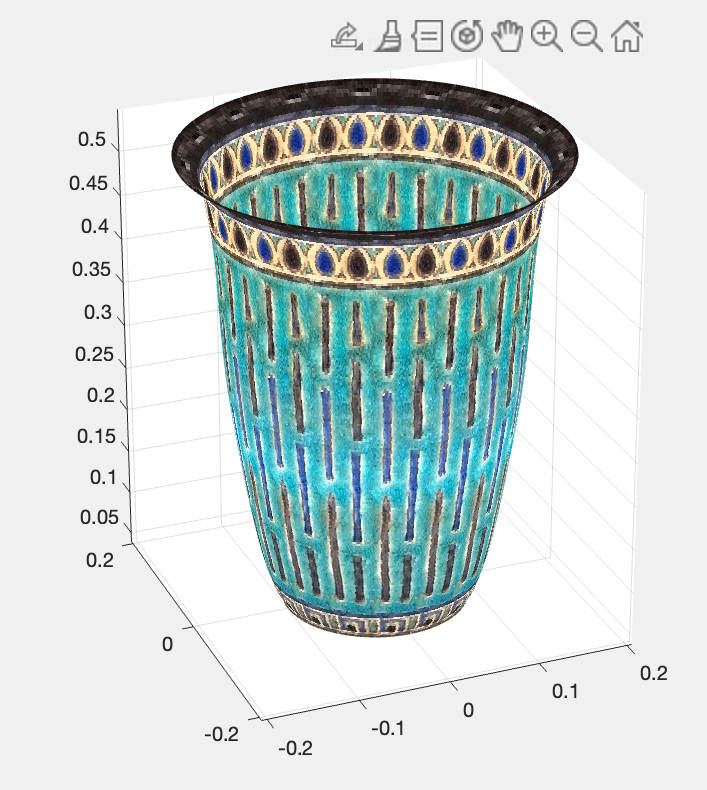
\includegraphics[height=5cm]{ourRes-20}\label{res4_3DOut:f2}}
	\caption{مدل سه‌بعدی بازسازی شده سوم}
	\label{res4_3DOut}
\end{figure}
\newline
در نمونه‌ی بعدی، شیء حاوی الگوی تکرارشونده‌ای نیست. این جسم (تصویر\ref{res5In:f1})، که یک بطری است، برای نمایش کاربرد الگوریتم ارائه‌شده در تکرار الگوی رویی برای قسمت پشت مدل سه‌بعدی آورده شده است. در شکل \ref{res5_bad} مدل سه‌بعدی بازسازی‌شده با استفاده از روش تکرار ساده الگوی رویی برای قسمت پشت آمده است. نتیجه‌ی این کار به نسبت مناسب است و مشکل زیادی ندارد. قطاع انتخاب شده برای الگوریتم ارائه‌شده در این حالت (تصویر \ref{res5In:f2}) همان الگوی رویی شیء در تصویر ورودی است که بدون بریدن به عنوان ورودی به الگوریتم ما داده می‌شود. 
\begin{figure}[h!]
	\centering
	\subfloat[تصویر اصلی شیء]{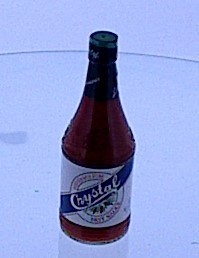
\includegraphics[height=4cm]{ourRes-21}\label{res5In:f1}}
	\qquad
	\subfloat[قطاع استخراج‌شده]{\includegraphics[height=4cm]{ourRes-22}\label{res5In:f2}}
	\caption{ورودی‌های پنجم الگوریتم ارائه‌شده}
	\label{res5In}
\end{figure}
\begin{figure}[h!]
	\centering
	\includegraphics[height=5cm]{ourRes-26}
	\caption{مدل سه‌بعدی بازسازی‌شده برای ورودی پنجم با استفاده از تکرار ساده طرح رویی برای پشت}
	\label{res5_bad}
\end{figure}

بافت تولید شده در شکل \ref{res5Out} آمده است. همانطور که مشخص است، تعداد تکرار قطاع برای این بافت برابر دو بوده است. در خط میانی مشاهده می‌شود که خط جداکننده سنگینی وجود ندارد و به نسبت دو قطاع به صورت همواری به یکدیگر متصل شده‌اند. به خصوص در قسمت برچسب بطری، گذار از قسمت بنفش به رنگ پس‌زمینه‌ی برچسب هموارتر شده است و خط محکمی وجود ندارد.
\begin{figure}[h!]
	\centering
	\includegraphics[height=5cm]{ourRes-23}
	\caption{بافت تولید شده از الگوریتم ارائه‌شده برای ورودی پنجم}
	\label{res5Out}
\end{figure}

شکل \ref{res5_3DOut} مدل سه‌بعدی بازسازی‌شده‌ی نهایی را در کنار مدل بازسازی شده با استفاده از روش تکرار ساده نمایش می‌دهد. همانطور که در مورد بافت تولید‌شده برای این شیء گفته‌شد، به نظر می‌آید با استفاده از الگوریتم ارائه‌شده، بافت اندکی هموارتر بوده و عملکردی تقریبا برابر با تکرار ساده بافت رویی برای قسمت پشت مدل سه‌بعدی داشته.
\begin{figure}[h!]
	\centering
	\subfloat[]{\includegraphics[height=5cm]{ourRes-24}\label{res5_3DOut:f1}}
	\qquad
	\subfloat[]{\includegraphics[height=5cm]{ourRes-25}\label{res5_3DOut:f2}}
	\caption{مدل سه‌بعدی بازسازی شده پنجم}
	\label{res5_3DOut}
\end{figure}

در انتها یک مثال آورده می‌شود که عملکرد الگوریتم ما مناسب نبوده است. شیء ورودی و قطاع استخراج‌شده از آن در شکل \ref{res6In} آمده است. همانطور که در تصویر قطاع مشخص است، قطاع طرح تکرارشونده را به صورت مناسب در بر گرفته، اما از سمت راست به چپ، در قسمت بالا‌ی قطاع، شدت نور در حال کاهش است و حاشیه‌ی سمت چپ قطاع با شروع سایه همراه بوده است. مشکل دیگری که دیده می‌شود، صاف نبودن خطوط پایینی الگو است که به علت مشکل در استخراج الگوی رویی پیش آمده. توانستیم با استفاده از روش رفع واپیچش خط‌های بالایی را صاف کنیم، اما خط‌های پایینی صاف نشدند.
\begin{figure}[h!]
	\centering
	\subfloat[تصویر اصلی شیء]{\includegraphics[height=4cm]{ourRes-27}\label{res6In:f1}}
	\qquad
	\subfloat[قطاع استخراج‌شده]{\includegraphics[height=4cm]{ourRes-28}\label{res6In:f2}}
	\caption{ورودی‌های ششم الگوریتم ارائه‌شده}
	\label{res6In}
\end{figure}

در شکل \ref{res6Out} بافت تولید شده برای این شیء آمده است. الگوریتم ما نتوانسته به صورت مناسب در قسمت بالا (به علت وجود سایه) و پایین (به علت صاف نبودن خطوط و وجود سایه) هموار کردن قطاع را انجام دهد. در قسمت میانی قطاع به علت صاف بودن و نبود سایه، هموار شدن به صورت مناسبی صورت گرفته است.
\begin{figure}[h!]
	\centering
	\includegraphics[height=5cm]{ourRes-30}
	\caption{بافت تولید شده از الگوریتم ارائه‌شده برای ورودی ششم}
	\label{res6Out}
\end{figure}

در تصویر \ref{res6_3DOut:f2} می‌توان مدل سه‌بعدی نهایی بعد از نگاشت بافت تولیدشده را دید. همانطور که در تصویر بافت هم دیدیم، مدل در قسمت بالا و پایین قطاع، ظاهر مناسبی ندارد و به صورت مناسب هموار نشده است. در تصویر \ref{res6_3DOut:f2} مدل نهایی تولید شده با استفاده از روش تکرار الگوی رویی برای پشتی آمده است که نشان می‌دهد عملکرد روش ما نسبت به این روش، بهتر بوده است.
\begin{figure}[h!]
	\centering
	\subfloat[روش تکرار]{\includegraphics[height=5cm]{ourRes-29}\label{res6_3DOut:f1}}
	\qquad
	\subfloat[الگوریتم ارائه‌شده]{\includegraphics[height=5cm]{ourRes-31}\label{res6_3DOut:f2}}
	\caption{مدل سه‌بعدی بازسازی شده ششم}
	\label{res6_3DOut}
\end{figure}

اولین علت این ضعف می‌تواند این موضوع باشد که الگوریتم ارائه‌شده تنها به حاشیه‌ها توجه می‌کند و نمی‌تواند ناسازگاری‌های الگو را در طول قطاع هموار کند. دومین علت نیز می‌تواند کم بودن مساحت در نظر گرفته شده برای ناحیه‌ی هم‌پوشانی باشد. با توجه به اینکه طول این ناحیه به صورت یک عدد ثابت در نظر گرفته شده، برای تصاویری که کیفیت بالاتر و تعداد پیکسل‌های بیشتری دارند، این مساحت می‌تواند به نسبت تعداد پیکسل‌های قطاع، کوچک باشد و باعث شود الگوریتم به درستی کار خود را انجام ندهد. در نظر گرفتن مساحت ناحیه‌ی هم‌پوشانی به صورت نسبتی از طول قطاع، امکان دارد نتایج را بهتر کند. البته باید دقت کرد این مساحت از تصویر ورودی الگو بیرون نزند. به طور مثال برای ورودی‌هایی که الگو برش‌ داده نمی‌شود، ناحیه‌ی هم‌پوشانی بزرگ می‌تواند نظم الگو را به هم بزند.

در انتها، جدول \ref{tab:timings} زمان اجرای روش ما برای ورودی‌های نمایش داده‌شده در این بخش را نمایش می‌دهد.
\newpage
\begin{table}[htbp]
	\caption{زمان اجرای الگوریتم}
	\label{tab:timings}
	\centering
	\onehalfspacing
	\begin{tabular}{ ||c c c c|| }
		\hline \rl{ورودی} & \rl{ابعاد قطاع} & \rl{تعداد تکرار قطاع} & \rl{مدت زمان (ثانیه)} \\ 
		\hline
		\hline \rl{ورودی اول \ref{res1In}} & \lr{$305*401$} & $12$ & $26.92$ \\ 
		\hline \rl{ورودی دوم \ref{res2In}} & \lr{$302*401$} & $8$ & $15.83$ \\ 
		\hline \rl{ورودی سوم \ref{res3In}} & \lr{$936*300$} & $3$ & $25.37$ \\ 
		\hline \rl{ورودی چهارم \ref{res4In}} & \lr{$192*200$} & $16$ & $5.61$ \\ 
		\hline \rl{ورودی پنجم \ref{res5In}} & \lr{$1270*200$} & $2$ & $12.09$ \\ 
		\hline \rl{ورودی ششم \ref{res6In}} & \lr{$476*500$} & $4$ & $24.59$ \\ 
		\hline
	\end{tabular}
\end{table}

		% فصل چهارم: نتایج
% !TeX root=../main.tex

\chapter{نتیجه‌گیری}
\label{section_conclusion}
در این پژوهش، روشی برای تولید بافت برای بازسازی سه‌بعدی از یک تصویر اشیاء با الگو‌های تکراری و دارای ساختار پیچیده، ارائه شد. این روش مبتنی بر حل یک مسئله خطی بهینه‌سازی در فضای گرادیان و در‌هم‌ریزی پواسون، برای گسترش افقی قطاع‌های الگو بود. در این پژوهش به دنبال بافت از قطاع‌های تکرار‌شونده‌ی الگو بودیم، به طوری که خطوط عمودی قابل مشاهده‌ای در مرزهای قطاع‌های مجاور وجود نداشته باشد. 
%
نشان دادیم با استفاده از این روش، اختلاف نوری یا سایر عناصر بصری را می توان در حین انتقال از یک قطاع الگو به قطاع بعدی حذف کرد، که منجر به تولید بافت نهایی جذاب‌تر از نظر بصری برای مدل سه بعدی می‌شود. نشان دادیم که با استفاده از روش ارائه‌شده، ایجاد بافت برای اشیاء با تعداد تکرار فرد در الگوی تکراری آنها، نتایج بهتری نسبت به استفاده از یک تکرار ساده از بافت جلویی در پشت دارد. مزیت دیگر رویکرد ما این بود که می‌توان آن را برای اشیاء با بخش‌های متنی در بافت خود استفاده کرد، جایی که استفاده از تکنیک آینه کردن برای یکسان‌سازی شرایط نوری باعث به هم ریختن بافت می‌شود. همانطور که در نتایج نشان داده شده است، انتخاب یک برش الگوی قابل اجرا برای نتیجه رویکرد ما بسیار مهم است. از آنجایی که روش ارائه‌شده بر نواحی مرزی قطاع متمرکز است، انتخاب یک برش الگو با تفاوت قابل‌توجه در روشنایی دو طرف قطاع منجر به ایجاد بافت‌هایی می‌شود که به مقدار مناسبی هموار نشده‌اند.

برای کارهای آینده، به جای تلاش برای برش الگو استخراج شده از بافت رویی شی، استخراج قطاع مستقیماً از تصویر شی و سپس اصلاح واپیچش این قطاع می‌تواند روشی برای دست‌یابی به نتایح مطلوب‌تری باشد. موضوع دیگری که می‌تواند برای انتخاب بهتر قطاع انجام شود، امتیاز دادن به مدل سه بعدی نهایی تولید شده بر اساس تفاوت بین مدل سه بعدی و تصویر ورودی و پیشنهاد بهترین نقاط برش در بافت جلویی استخراج شده است. یکسان‌سازی شرایط نوری در طول قطاع، به جای تمرکز فقط بر حاشیه‌های قطاع، جنبه دیگری از روش ما است که نیاز به مطالعه بیشتر دارد. اینکار می‌تواند با انتخاب ناحیه هم‌پوشانی به صورت پویا یا اضافه کردن قسمت‌های پیش‌پردازش به روند اجرای روش، انجام شود. بخش دیگری که می‌تواند باعث بهبود روش ارائه‌شده شود، پیاده‌سازی روش‌های دیگر در قسمت حل سیستم معادلات خطی نیز می‌تواند باعث افزایش سرعت این روش شده و زمینه‌ی مناسبی برای ادامه‌ی پژوهش انجام شده باشد.		% فصل پنجم: جمع‌بندی

% مراجع
% اگر از استیل‌های natbib استفاده می‌کنید باید دو خط را در فایل commands.tex تغییر دهید.
\pagestyle{empty}
{
\small
\onehalfspacing
\bibliographystyle{plain-fa} % or plainnat-fa for author-date
\bibliography{./tex/MyReferences}
}

\pagestyle{fancy}

% \appendix
% فصلهای پس از این قسمت به عنوان ضمیمه خواهند آمد.

% دستورات لازم برای تبدیل «فصل آ» به «پیوست آ» در فهرست مطالب
\addtocontents{toc}{
    \protect\renewcommand\protect\cftchappresnum{\appendixname~}%
    \protect\setlength{\cftchapnumwidth}{\mylenapp}}
    
% دستورات لازم برای شماره‌گذاری صفحات پیوست‌ها بشکل آ-۱ (فعلا با glossaries سازگار نیست)
% \let\Chapter\chapter
%\pretocmd{\chapter}{
%  \clearpage
%  \pagenumbering{arabic}
%  \renewcommand*{\thepage}{\rl{\thechapter-\arabic{page}}}}{}{}
%%%%%%%%%%%%%%%%%%%%%%%%%%%%%%%%%%%%%
        

%% !TeX root=../main.tex

\chapter{آشنایی سریع با برخی دستورات لاتک}
\label{app:latexIntro}
%\thispagestyle{empty}
در این فصل ویژگی‌های مهم و پرکاربرد زی‌پرشین و لاتک معرفی می‌شود. برای راهنمایی بیشتر و به‌کاربردن ویژگی‌های پیشرفته‌تر به راهنمای زی‌پرشین و راهنمای لاتک مراجعه کنید. برای آگاهی از دستورات لاتک که این خروجی را تولید کرده‌اند فایل \lr{appendix1.tex} را ملاحظه فرمایید.
\footnote{بیشتر مطالب این بخش از مثال 
\lr{xepersian\_example.tex}
گرفته شده‌اند که توسط آقای امیرمسعود پورموسی آماده شده است.}

\section{بندها و زیرنویس‌ها}
هر جایی از نوشتهٔ خود، اگر می‌خواهید به سر سطر بروید و یک بند (پاراگراف) تازه را آغاز کنید، باید یک خط را خالی بگذارید%
\footnote{یعنی دوبار باید کلید \lr{Enter} را بزنید.}
 مانند این:

حالا که یک بند تازه آغاز شده است، یک زیرنویس انگلیسی%
\LTRfootnote{English Footnote!}
 هم می‌نویسیم!
\section{فرمول‌های ریاضی}
\label{formula}

اینجا هم یک فرمول می‌آوریم که شماره دارد:
\begin{equation}\label{eq:yek}
A=\frac{c}{d}+\frac{q^2}{\sin(\omega t)+\Omega_{12}}
\end{equation}
در لاتک می‌توان به کمک فرمان 
\lr{\textbackslash label\{\}}
به هر فرمول یک نام نسبت داد. در فرمول بالا نام \lr{eq:yek} را برایش گذاشته‌ایم (پروندهٔ \lr{tex} همراه با این مثال را ببینید). این نام ما را قادر می‌کند که بعداً بتوانیم با فرمان
\lr{\textbackslash ref\{eq:yek\}}
به آن فرمول با شماره ارجاع دهیم. یعنی بنویسیم فرمول \ref{eq:yek}. 
لاتک خودش شمارهٔ این فرمول‌ها را مدیریت می‌کند.\footnote{یعنی اگر بعداً فرمولی قبل از این فرمول بنویسیم، خودبه‌خود شمارهٔ این فرمول و شمارهٔ ارجاع‌ها به این فرمول یکی زیاد می‌شود. دیگر نگران شماره‌گذاری فرمول‌های خود نباشید!} این هم یک فرمول که شماره ندارد:
$$A=|\vec{a}\times \vec{b}| + \sum_{n=0}^\infty C_{ij}$$

این هم عبارتی ریاضی مانند 
$\sqrt{a^2+b^2}$
 که بین متن می‌آید.
\subsection{یک زیربخش}
\label{zirbakhsh}

این زیربخش \ref{zirbakhsh} است؛ یعنی یک بخش درون بخش \ref{formula} است.
\subsubsection{یک زیرزیربخش}
این هم یک زیرزیربخش است. در لاتک می‌توانید بخش‌های تودرتو در نوشته‌تان تعریف کنید تا ساختار منطقی نوشته را به خوبی نشان دهید. می‌توانید به این بخش‌ها هم با شماره ارجاع دهید، مثلاً بخش فرمول‌های ریاضی شماره‌اش \ref{formula} است.
\section{نوشته‌های فارسی و انگلیسی مخلوط}
نوشتن یک کلمهٔ انگلیسی بین متن فارسی بدیهی است، مانند Example در این جمله.\footnote{هرچند بهتر است باز هم آن کلمه را مانند \lr{Example} در این جمله بنویسید.}
نوشتن یک عبارت چندکلمه‌ای مانند
 \lr{More than one word} کمی پیچیده‌تر است.

اگر ناگهان تصمیم بگیرید که یک بند کاملاً انگلیسی را بنویسید، باید:
\begin{latin}
This is an English paragraph from left to right. You can write as much as you want in it.
\end{latin}
\section{افزودن تصویر به نوشته}
پروندهٔ تصویر دلخواه خود را در کنار پروندهٔ \lr{tex} قرار دهید. سپس به روش زیر تصویر را در نوشتهٔ خود بیاورید:
\begin{latin}
\begin{verbatim}
\includegraphics{YourImageFileName}
\end{verbatim}
\end{latin}
به تصویرها هم مانند فرمول‌ها و بخش‌ها می‌توان با شماره ارجاع داد. مثلاً تصویر \ref{fig:shir} یک شیر علاقه‌مند به لاتک را در حال دویدن نشان می‌دهد. برای جزئیات بیشتر دربارهٔ روش گذاشتن تصویرها در نوشته باید راهنماهای لاتک را بخوانید.
\begin{figure}[ht]
\centerline{\includegraphics[width=5cm]{lion}}
\caption{در این تصویر یک شیر علاقه‌مند به لاتک را در حال دویدن می‌بینید.}
\label{fig:shir}
\end{figure}

به تصویرها هم مانند فرمول‌ها و بخش‌ها می‌توان با شماره ارجاع داد. مثلاً تصویر بالا شماره‌اش \ref{fig:shir} است. برای جزئیات بیشتر دربارهٔ روش گذاشتن تصویرها در نوشته باید راهنماهای لاتک را بخوانید.

\section{محیط‌های شمارش و نکات}
برای فهرست‌کردن چندمورد، اگر ترتیب برایمان مهم نباشد:
\begin{itemize}
\item مورد یکم
\item مورد دوم
\item مورد سوم
\end{itemize}
و اگر ترتیب برایمان مهم باشد:
\begin{enumerate}
\item مورد یکم
\item مورد دوم
\item مورد سوم
\end{enumerate}
می‌توان موردهای تودرتو داشت:
\begin{enumerate}
\item مورد ۱
\item مورد ۲
\begin{enumerate}
\item مورد ۱ از ۲
\item مورد ۲ از ۲
\item مورد ۳ از ۲
\end{enumerate}
\item مورد ۳
\end{enumerate}
شماره‌گذاری این موردها را هم لاتک انجام می‌دهد.

\section{تعریف و قضیه}
برای ذکر تعریف، قضیه و مثال مثالهای ذیل را ببینید.
\begin{definition}
مجموعه همه ارزیابی‌های  (پیوسته)  روی $(X,\tau)$، دامنه توانی احتمالی
\index{دامنه توانی احتمالی}
$ X $
نامیده می‌شود.
\end{definition}
\begin{theorem}[باناخ-آلااغلو]
\index{قضیه باناخ-آلااغلو}
اگر $ V $ یک همسایگی $ 0 $ در فضای برداری 
\index{فضای!برداری}
 توپولوژیکی $ X $ باشد و 
\begin{equation}\label{eq1}
K=\left\lbrace \Lambda \in X^{*}:|\Lambda x|\leqslant 1 ; \ \forall x\in V\right\rbrace,
\end{equation}
آنگاه $ K $،  ضعیف*-فشرده است که در آن، $ X^{*} $ دوگان
\index{فضای!دوگان}
 فضای برداری توپولوژیکی $ X $ است به ‌طوری که عناصر آن،  تابعی‌های 
خطی پیوسته
\index{تابعی خطی پیوسته}
 روی $X$ هستند.
\end{theorem}
تساوی \eqref{eq1} یکی از مهم‌ترین تساوی‌ها در آنالیز تابعی است که در ادامه، به وفور از آن استفاده می‌شود.
\begin{example}
برای هر فضای مرتب، گردایه 
$$U:=\left\lbrace U\in O: U=\uparrow U\right\rbrace $$
از مجموعه‌های بالایی باز، یک توپولوژی تعریف می‌کند که از توپولوژی اصلی، درشت‌تر  است.
\end{example}
حال تساوی 
\begin{equation}\label{eq2}
\sum_{n=1}^{+\infty} 3^{n}x+7x=\int_{1}^{n}8nx+\exp{(2nx)}
\end{equation}
را در نظر بگیرید. با مقایسه تساوی \eqref{eq2} با تساوی \eqref{eq1} می‌توان نتیجه گرفت که ...


\section{چگونگی نوشتن و ارجاع به مراجع}
\label{Sec:Ref}


در لاتک به راحتی می‌توان مراجع خود را نوشت و به آنها ارجاع داد. به عنوان مثال برای معرفی کتاب گنزالس \cite{Gonzalez02book} به عنوان یک مرجع می‌توان آنرا به صورت زیر معرفی نمود:

\singlespacing
\begin{LTR}
\begin{verbatim}
\bibitem{Gonzalez02book}
Gonzalez, R.C., and Woods, R.E. {\em Digital Image Processing}, 3rd ed..
Prentice-Hall, Inc., Upper Saddle River, NJ, USA, 2006.
\end{verbatim}
\end{LTR}
\doublespacing

در دستورات فوق \lr{Gonzalez02book}  برچسبی است که به این مرجع داده شده است و با استفاده از دستور 
\verb!\cite{Gonzalez02book}!
می‌توان به آن ارجاع داد؛ بدون این که شماره‌اش را در فهرست مراجع‌مان بدانیم.

اگر این اولین مرجع ما باشد در قسمت مراجع به صورت زیر خواهد آمد:\\
\includegraphics[width=\textwidth]{gonzalez.png}

این شیوهٔ تعریف مراجع بسیار ابتدایی است و اگر فرمت مراجع، ترتیب یا تعداد آنها را خواسته باشید تغییر دهید، به عنوان مثال ابتدا حرف اول نام نویسنده بیاید و سپس نام خانوادگی، باید همه کارها را به صورت دستی انجام دهید!
چون در یک \پ یا مقاله باید کنترل کاملی بر مراجع خود داشته باشید و به راحتی بتوانید قالب مراجع را عوض کنید، بنابراین می‌بایست از \lr{Bib\TeX} استفاده کنید که درپیوست  \ref{app:refMan} به  آن پرداخته خواهد شد.
		% پیوست اول: آشنایی مقدماتی با لاتک
%% !TeX root=../main.tex

\chapter{‌جدول، نمودار و الگوریتم در لاتک}
\label{app:latex:more}
%\thispagestyle{empty}

در این بخش نمونه مثالهایی از جدول، شکل، نمودار، الگوریتم و معادلات ریاضی را در لاتک خواهیم دید.
دقت کنید که در پایان‌نامه‌ها و مقالات، باید قاعدهٔ «ارجاع به جلو%
\LTRfootnote{Forward Referencing}»
رعایت شود؛ یعنی ابتدا در متن به شمارهٔ شکل، جدول یا معادله اشاره شود و بعد از آن (زیر آن) خود شکل، جدول یا معادله رسم شود. (توضیحات بیشتر در قسمت
\ref{sec:floatObjs}).

\section{جدول}
دستور اصلی برای رسم جدول در لاتک 
\verb|tabular|
می‌باشد که جدول
\eqref{tab:motionModels}
با استفاده از آن کشیده شده است؛ در
\verb|tabular|
عرض جدول برابر با مجموع عرض ستون‌ها و حداکثر مساوی عرض متن است.
\begin{table}[ht]
\caption{مدلهای تبدیل.}
\label{tab:motionModels}
\centering
\onehalfspacing
\begin{tabular}{|r|c|l|r|}
	\hline نام مدل & درجه آزادی & تبدیل مختصات & توضیح \\ 
	\hline انتقالی & ۲ & $\begin{aligned} x'=x+t_x \\ y'=y+t_y \end{aligned}$  &  انتقال دوبعدی\\ 
	\hline اقلیدسی & ۳ & $\begin{aligned} x'=x\cos\theta - y\sin\theta+t_x \\ y'=x\sin\theta+y\cos\theta+t_y \end{aligned}$  &  انتقالی+دوران \\ 
	\hline 
\end{tabular} 
\end{table}

برای اینکه عرض جدول قابل کنترل باشد، باید از دستورات
\verb|tabularx|،
\verb|tabulary| یا
\verb|tabu|
استفاده کرد که راهنمای آنها در اینترنت وجود دارد.
مثلاً جدول
\ref{tab:motionModelsCont}
با
\verb|tabularx|
رسم شده که عرض جدول در آن ثابت بوده و ستون‌های از نوع
\verb|X|
عرض خالی جدول را پر می‌کنند.
\begin{table}[ht]
	\caption{مدلهای تبدیل دیگر.}
	\label{tab:motionModelsCont}
	\centering
	\onehalfspacing
	\begin{tabularx}{\textwidth}{|r|c|l|X|}
		\hline نام مدل & درجه آزادی & تبدیل مختصات & توضیح \\ 
		\hline مشابهت & ۴ & $\begin{aligned} x'=sx\cos\theta - sy\sin\theta+t_x \\ y'=sx\sin\theta+sy\cos\theta+t_y  \end{aligned}$  & اقلیدسی+تغییرمقیاس \\ 		
		\hline آفین & ۶ & $\begin{aligned} x'=a_{11}x+a_{12}y+t_x \\ y'=a_{21}x+a_{22}y+t_y \end{aligned}$  & مشابهت+اریب‌شدگی \\
		\hline
	\end{tabularx}
\end{table}

\section{معادلات ریاضی و ماتریس‌ها}
تقریباً هر آنچه دانشجویان برای نوشتن فرمول‌های ریاضی لازم دارند، در کتاب 
\lr{mathmode}
آمده است. کافیست در خط فرمان، دستور زیر را وارد کنید:
\begin{latin}
	\texttt{texdoc mathmode}
\end{latin}
متن زیر شامل انواعی از اشیاء ریاضی است که با ملاحظه کدش می‌توانید با دستورات آن آشنا شوید.\\
شناخته‌شده‌ترین روش تخمین ماتریس هوموگرافی الگوریتم تبدیل خطی مستقیم (\lr{DLT\LTRfootnote{Direct Linear Transform}}) است.  فرض کنید چهار زوج نقطهٔ متناظر در دو تصویر در دست هستند،  $\mathbf{x}_i\leftrightarrow\mathbf{x}'_i$   و تبدیل با رابطهٔ
  $\mathbf{x}'_i = H\mathbf{x}_i$
  نشان داده می‌شود که در آن:
\[\mathbf{x}'_i=(x'_i,y'_i,w'_i)^\top  \]
و
\[ H=\left[
\begin{array}{ccc}
h_1 & h_2 & h_3 \\ 
h_4 & h_5 & h_6 \\ 
h_7 & h_8 & h_9
\end{array} 
\right]\]
رابطه زیر را برای الگوریتم  \eqref{alg:DLT} لازم داریم.
\begin{equation}
\label{eq:DLT_Ah}
\left[
\begin{array}{ccc}
	0^\top & -w'_i\mathbf{x}_i^\top & y'_i\mathbf{x}_i^\top \\ 
	w'_i\mathbf{x}_i & 0^\top & -x'_i\mathbf{x}_i^\top \\ 
	- y'_i\mathbf{x}_i^\top & x'_i\mathbf{x}_i^\top & 0^\top
\end{array} 
\right]
\left(
\begin{array}{c}
	\mathbf{h}^1 \\ 
	\mathbf{h}^2 \\ 
	\mathbf{h}^3
\end{array} 
\right)=0
\end{equation}

\section{الگوریتم}

\subsection{الگوریتم ساده با دستورهای فارسی}
با مفروضات فوق، الگوریتم \lr{DLT} به صورت نشان داده شده در الگوریتم \eqref{alg:DLT}  خواهد بود.
\begin{algorithm}[ht]
\onehalfspacing
\caption{الگوریتم \lr{DLT} برای تخمین ماتریس هوموگرافی.} \label{alg:DLT}
\begin{algorithmic}[1]
\REQUIRE $n\geq4$ زوج نقطهٔ متناظر در دو تصویر 
${\mathbf{x}_i\leftrightarrow\mathbf{x}'_i}$،\\
\ENSURE ماتریس هوموگرافی $H$ به نحوی‌که: 
$\mathbf{x}'_i = H \mathbf{x}_i$.
  \STATE برای هر زوج نقطهٔ متناظر
$\mathbf{x}_i\leftrightarrow\mathbf{x}'_i$ 
ماتریس $\mathbf{A}_i$ را با استفاده از رابطهٔ \ref{eq:DLT_Ah} محاسبه کنید.
  \STATE ماتریس‌های ۹ ستونی  $\mathbf{A}_i$ را در قالب یک ماتریس $\mathbf{A}$ ۹ ستونی ترکیب کنید. 
  \STATE تجزیهٔ مقادیر منفرد \lr{(SVD)}  ماتریس $\mathbf{A}$ را بدست آورید. بردار واحد متناظر با کمترین مقدار منفرد جواب $\mathbf{h}$ خواهد بود.
  \STATE  ماتریس هوموگرافی $H$ با تغییر شکل $\mathbf{h}$ حاصل خواهد شد.
\end{algorithmic}
\end{algorithm}

\subsection{الگوریتم پیچیده و تودرتو با دستورهای فارسی}
الگوریتم \ref{alg:simulation-random}، یک الگوریتم ترکیبی و تودرتو است که با کمک دستورهای بستهٔ \lr{algorithmic} نوشته شده است.

\begin{algorithm}[p]
    \onehalfspacing
    \caption{الگوریتم اجرای برنامهٔ شبیه‌سازی}
    \label{alg:simulation-random}
    \begin{algorithmic}[1]
        \REQUIRE زمان $t_{max}$ به عنوان زمان لازم برای انجام شبیه سازی،\\
        \REQUIRE  گراف شبکه برای شبیه سازی،
        \ENSURE جدول تغییرات گراف از لحظهٔ ۰ تا t.
        \FOR {تمام لحظات در بازهٔ ۰ تا $t_{max}$}
            \FOR {تمام پیوند‌ها}
                \STATE محاسبهٔ ضریب و نرخ انتقال پیوند
                \STATE محاسبهٔ کیفیت و نرخ یادگیری
            \ENDFOR
            \FOR {تمام گره‌ها}
                \STATE محاسبهٔ نرخ انتقال گره
                \STATE محاسبهٔ وضعیت جدید
            \ENDFOR
            \IF {تغییرات از مقدار $\delta$ کمتر است}
                \STATE شکستن حلقه
                \COMMENT{این شرط برای پایان قبل از رسیدن به محدودیت زمانی است، اگر تغییرات کمتر از $\delta$ باشد}
            \ELSIF {زمان اجرای برنامه بیش از حد طول کشیده \AND $t>100$}
                \STATE شکستن حلقه
            \ENDIF
        \ENDFOR
        \PRINT {زمان اجرای برنامه}
        \RETURN {ماتریس تغییرات زمانی}
    \end{algorithmic}
\end{algorithm}

\subsection{الگوریتم با دستورهای لاتین}
الگوریتم \ref{alg:RANSAC} یک الگوریتم با دستورهای لاتین است.

\begin{algorithm}[ht]
\onehalfspacing
\caption{الگوریتم \lr{RANSAC} برای تخمین ماتریس هوموگرافی.} \label{alg:RANSAC}
\begin{latin}
\begin{algorithmic}[1]
\REQUIRE $n\geq4$ putative correspondences, number of estimations, $N$, distance threshold $T_{dist}$.\\
\ENSURE Set of inliers and Homography matrix $H$.
\FOR{$k = 1$ to $N$}
  \STATE Randomly choose 4 correspondence,
  \STATE Check whether these points are colinear, if so, redo the above step
  \STATE Compute the homography $H_{curr}$ by DLT algorithm from the 4 points pairs,
  \STATE $\ldots$ % الگوریتم کامل نیست
  \ENDFOR
  \STATE Refinement: re-estimate H from all the inliers using the DLT algorithm.
\end{algorithmic}
\end{latin}
\end{algorithm}

\section{کد}
درج کد به زبان‌های مختلف به سادگی امکان‌پذیر است. برنامه
\ref{code:matlabEx}
یک قطعه کد
\lr{MATLAB}
را نشان می‌دهد.
\begin{figure}[ht]
	\begin{LTR}
        \singlespacing
		\lstinputlisting[language=MATLAB, caption={نمونه کد \lr{MATLAB}}, label={code:matlabEx}]{MatlabExample.m}
        % \doublespacing
	\end{LTR}
\end{figure}

\section{تصویر}
نمونهٔ یک تصویر را در فصل قبل دیدیم. دو تصویر شیر کنار هم را نیز در شکل
\ref{fig:twoLion}
مشاهده می‌کنید.
\begin{figure}[ht]
\centering 
\subfloat[شیر ۱]{ \label{fig:twolion:one}
\includegraphics[width=0.3\textwidth]{lion}}
%\hspace{2mm}
\subfloat[شیر ۲]{ \label{fig:twolion:two}
\includegraphics[width=0.3\textwidth]{lion}}%
\caption{دو شیر}
\label{fig:twoLion} %% label for entire figure
\end{figure}

\section{نمودار}
لاتک بسته‌هایی با قابلیت‌های زیاد برای رسم انواع مختلف نمودارها دارد. مانند بسته‌های \lr{Tikz} و  \lr{PSTricks}. توضیح اینها فراتر از این پیوست کوچک است.%
\footnote{
مثال‌هایی از بکارگیری بسته
\lr{Tikz}
را می‌توانید در
\url{http://www.texample.net/tikz/examples/}
ببینید. توصیه می‌شود دانشجویانی که قصد درج اشکالی مانند گراف را در سند خود دارند، مثالهایی از سایت مذکور را ملاحظه فرمایند.
}
یک نمودار رسم شده با بستهٔ 
\lr{TikZ}
 در شکل 
\ref{fig:parabola}
نشان داده شده است.
\begin{figure}[t]
\centering
\begin{tikzpicture}[scale=2.5]
  \shade[top color=blue,bottom color=gray!50] 
      (0,0) parabola (1.5,2.25) |- (0,0);
  \draw (1.05cm,2pt) node[above] 
      {$\displaystyle\int_0^{3/2} \!\!x^2\mathrm{d}x$};

  \draw[style=help lines] (0,0) grid (3.9,3.9)
       [step=0.25cm]      (1,2) grid +(1,1);

  \draw[->] (-0.2,0) -- (4,0) node[right] {$x$};
  \draw[->] (0,-0.2) -- (0,4) node[above] {$f(x)$};

  \foreach \x/\xtext in {1/1, 1.5/1\frac{1}{2}, 2/2, 3/3}
    \draw[shift={(\x,0)}] (0pt,2pt) -- (0pt,-2pt) node[below] {$\xtext$};

  \foreach \y/\ytext in {1/1, 2/2, 2.25/2\frac{1}{4}, 3/3}
    \draw[shift={(0,\y)}] (2pt,0pt) -- (-2pt,0pt) node[left] {$\ytext$};

  \draw (-.5,.25) parabola bend (0,0) (2,4) node[below right] {$x^2$};
\end{tikzpicture}
\caption{یک نمودار زیبا با ارقام فارسی و قابلیت بزرگ‌نمایی بسیار، بدون از دست دادن کیفیت.}
\label{fig:parabola}
\end{figure}

\section{نحوه قرارگیری اشیای شناور}
\label{sec:floatObjs}
شکل‌ها، جداول و الگوریتم‌ها در لاتک اشیای شناور محسوب می‌شوند؛ یعنی خود لاتک تصمیم می‌گیرد آنها را در کجای صفحه ترسیم کند تا زیباتر باشد. اما می‌توان به لاتک توصیه کرد که آن را در قسمت خاصی از صفحه رسم کند. برای اینکه قاعدهٔ «ارجاع به جلو» رعایت شود باید فقط از پرچم
\verb|[ht]|
استفاده کرد، که می‌گوید اگر جا شد شکل را دقیقاً در همین مکان و در غیراینصورت در بالای صفحه بعد رسم کن.
بنابراین دستورات درج تصویر، جدول و الگوریتم به صورت زیر باید باشند:

\begin{latin}
\begin{verbatim}
	\begin{figure/table/algorithm}[ht]
		...
	\end{figure/table/algorithm}
\end{verbatim}
\end{latin}
		% پیوست دوم: جدول، نمودار و الگوریتم در لاتک
%% !TeX root=../main.tex
\chapter{مراجع، واژه‌نامه و حاشیه‌نویسی}
\label{app:refMan}
%\thispagestyle{empty}

\section{مراجع و نقل‌قول‌ها}
\label{sec:refUsage}
منابعِ پایان‌نامه، پایه و اساس تحقیق شما به حساب می‌آیند و ضرورت انجام مطالعه و روش‌های به کار رفته در بسیاری از قسمت‌های آن، به کمک منابع صورت می‌گیرد. در استفاده از مراجع علمی در پایان‌نامه، باید سعی کنید بیشتر از
\textbf{منابع چاپ‌شده و مهم}
استفاده کنید و
\emph{ارجاع به داده‌های چاپ نشده، خلاصه‌ها و پایان‌نامه‌ها، سبب به‌هم‌خوردگی و کاهش اعتبار قسمت ارجاع منابع می‌شود.}
استفاده از منابع و نقل قول‌هایی به تحقیق شما ارزش می‌دهند که
\textbf{در راستای هدف تحقیق بوده و به آن اعتبار ببخشند.}
برخی از دانش‌جویان تصوّر می‌کنند که کثرت نقل‌قول‌ها و ارجاعات زیاد، مهم‌ترین معیار علمی شدن پایان‌نامه است؛ حال آنکه استناد به تعداد کثیری از منابع بدون مطالعه دقیق آنها و استفادهٔ مستقیم در پایان‌نامه، می‌تواند نشان‌دهندهٔ عدم احساس امنیت نویسنده باشد!

دو روش برای استفاده از نتایج، جملات، داده‌ها و روش‌های دیگران وجود دارد. یکی نقل‌قول مستقیم و دقیق است و دیگری استفاده غیرمستقیم در متن مقاله، که در ادامه به قواعد این دو نوع نقل‌قول و ارجاع‌دهی اشاره می‌کنیم:
\begin{description}
	\item[نقل‌قول مستقیم:]
	نقل‌قول مستقیم باید دقیق و بدون هیچ تغییری در جملات باشد. بهتر است این‌گونه نقل‌قول‌ها تا حد امکان کوتاه باشد. جملات کوتاه داخل گیومه قرار می‌گیرند و باید به منبع دقیق آن، طبق روش ارجاع‌دهی به منابع، اشاره شود. به عنوان مثال در
	\cite{persianbib87userguide}
	آمده است که:
	\begin{quote}
		«با استفاده از فیلد
		\lr{AUTHORFA}
		می‌توان معادل فارسی نام نویسندگان مقالات لاتین را در متن داشت. معمولاً در اسناد فارسی خواسته می‌شود که پس از ذکر معادل فارسی نام نویسنده، نام لاتین نویسنده(ها) به عنوان پاورقی درج شود
		\citep{persianbib87userguide}.»
	\end{quote}
	\item[نقل‌قول غیرمستقیم:]
	نقل‌قول غیرمستقیم به معنی استفاده از ایده‌ها، نتایج، روش‌ها و داده‌های دیگران در درون متنِ پایان‌نامه، ولی به سبک خودتان و متناسب و هماهنگ با روند پایان‌نامهٔ شماست. در این حالت نیز باید متناسب با شیوهٔ ارجاع‌دهی به آن استناد شود.
\end{description}

با توجه به وجود سبک‌های مختلف ارجاع‌دهی، باید
\textbf{روش قابل قبول و یکسانی}
در طول پایان‌نامه برای اشاره به مراجع در متن و همچنین تهیه فهرست مراجع در انتهای پایان‌نامه بکار رود. مثلاً برای پایان‌نامه‌های مهندسی می‌توان از سبک ارجاع‌دهی
\lr{IEEE}%
\LTRfootnote{\url{http://www.ieee.org/documents/ieeecitationref.pdf}}
یا
\lr{acm}
استفاده کرد. طبیعتاً باید تناظر یک‌به‌یک بین فهرست مراجع در انتهای گزارش و مراجع مورد استفاده در متن باشد%
\footnote{البته گاهی ممکن است محقق مرجعی را مورد مطالعه قرار داده لیکن در متن به آن اشاره نکرده باشد؛ برخی معتقدند در این موارد نیز آوردن آن در فهرست مراجع، اشکالی ندارد، به این شرط که از عنوان «فهرست منابع» به جای «فهرست مراجع» استفاده شود.}.

برای سهولت مدیریت مراجعِ \پ%
، اکیداً توصیه می‌شود از یک ابزار «مدیریت منابع» (با خروجی
\texorpdfstring{\lr{Bib\TeX}}{Bib\TeX}%
) همچون
\lr{Mendeley}،
\lr{Zotero},
\lr{EndNote}
یا
\lr{Citavi}
استفاده کنید.

\subsection{ مدیریت مراجع با  \texorpdfstring{\lr{Bib\TeX}}{Bib\TeX}}
در بخش \ref{Sec:Ref} اشاره شد که با دستور 
 \lr{\textbackslash bibitem}
  می‌توان یک مرجع را تعریف نمود و با فرمان
 \lr{\textbackslash cite}
  به آن ارجاع داد. این روش برای تعداد مراجع زیاد و تغییرات آنها مناسب نیست. برای مدیریت منابع زیاد، سه بستهٔ
\lr{BibTeX} (پیش‌فرض),
\lr{natbib}
(ارجاع‌دهی در متن به صورت نویسنده-سال)
و \lr{BibLaTeX} (جدید و منعطف‌پذیر)
وجود دارند. در ادامه توضیحاتی در مورد مدیریت منابع با \lr{BibTeX} و \lr{natbib} در زی‌پرشین خواهیم آورد که همراه با توزیع‌های معروف تِک عرضه می‌شوند
\footnote{روش \lr{BibLaTeX} هنوز برای متون فارسی به درستی ترجمه نشده است.}.

یکی از روش‌های قدرتمند و انعطاف‌پذیر برای نوشتن مراجعِ مقالات و مدیریت مراجع در لاتک، استفاده از  \lr{BibTeX} است.
 روش کار با بیب‌تک به این صورت است که مجموعهٔ همهٔ مراجعی را که در \پ استفاده کرده یا خواهیم کرد، 
در پروندهٔ جداگانه‌ای با پسوند
\lr{bib}
نوشته و به آن فایل در سند خودمان به صورت مناسب لینک می‌دهیم.
 کنفرانس‌ها یا مجله‌های گوناگون برای نوشتن مراجع، قالب‌ها یا قراردادهای متفاوتی دارند که به آنها استیل‌های مراجع گفته می‌شود.
 در این حالت به کمک ‌استیل‌های بیب‌تک خواهید توانست تنها با تغییر یک پارامتر در پروندهٔ ورودی خود، مراجع را مطابق قالب موردنظر تنظیم کنید. 
 بیشتر مجلات و کنفرانس‌های معتبر یک فایل سبک
 (\lr{BibTeX Style})
با پسوند \lr{bst} در وب‌گاه خود می‌گذارند که برای همین منظور طراحی شده است.

به جز نوشتن مقالات، این سبک‌ها کمک بسیار خوبی برای تهیهٔ مستندات علمی همچون پایان‌نامه‌هاست که فرد می‌تواند هر قسمت از کارش را که نوشت مراجع مربوطه را به بانک مراجع خود اضافه نماید. با داشتن چنین بانکی از مراجع، وی خواهد توانست به راحتی یک یا چند ارجاع به مراجع و یا یک یا چند بخش را حذف یا اضافه ‌نماید؛ 
مراجع به صورت خودکار مرتب شده و
\textbf{فقط مراجع ارجاع داده شده در قسمت کتاب‌نامه خواهندآمد.}
قالب مراجع به صورت یکدست مطابق سبک داده شده بوده و نیازی نیست که کاربر درگیر قالب‌دهی به مراجع باشد. 

\subsection{سبک‌های مورد تأیید دانشگاه تهران}
طبق «دستورالعمل نگارش و تدوین پایان‌نامه» دانشگاه تهران در
\cite{UTThesisGuide}،
ارجاع در متن می‌تواند مطابق با هر یک از دو الگوی هاروارد یا ونکوور باشد:
\singlespacing
\begin{description}
	\item[سیستم نویسنده-سال (هاروارد):]
	ذکر نام نویسنده و سال نشر در متن. در این الگو مراجع بر اساس حروف الفبا تنظیم می‌گردند.
	\item[سیستم شماره‌دار (ونکوور):]
	ارجاع به مراجع به کمک شماره در متن. در این الگو شماره هر مرجع به ترتیب ظاهر شدن آن در متن در داخل کروشه قرار می‌گیرد. فهرست مراجع نیز بر اساس شماره مرجع (نه حروف الفبا) تنظیم می‌گردد.
\end{description}
\doublespacing

در مدیریت منابع با
\lr{\textbf{BibTeX}}،
ارجاع‌ها در متن تنها به شکل
\textbf{شماره‌دار (ونکوور)}
امکان‌پذیر است، گرچه فهرست مراجع می‌تواند با روش‌های مختلف مرتب شود. اگر بخواهیم ارجاع‌ها در متن به صورت
\textbf{نویسنده-سال (هاروارد)}
باشد باید از بستهٔ
\lr{\textbf{natbib}}\LTRfootnote{Natural Sciences Citations \& References}
و استیل‌های مختلف آن استفاده کنیم.

هنگام استفاده از روش نویسنده-سال نوع پرانتزگذاری‌ها در وسط و انتهای جمله با هم فرق خواهد داشت. به مثال زیر مطابق با دستورالعمل
\cite{UTThesisGuide}
توجه کنید:

\textit{
ابتدا
\cite{Khalighi87xepersian}
بستهٔ زی‌پرشین را برای حروف‌چینی فارسی اختراع کرد. بعدها سبک‌های ارجاع‌دهی فارسی و قالب‌های پایان‌نامه نیز مبتنی بر آن ساخته شد
\citep{persianbib87userguide}.
ارجاع‌دهی به مراجع لاتین نیز در زی‌پرشین امکان‌پذیر است. مثلاً
\citelatin{Gonzalez02book}
یک کتاب انگلیسی است و به راحتی به مقالات انگلیسی نیز می‌توان ارجاع داد
\citeplatin{kim2016integrated}.}

در این مثال، ۴ ارجاع در وسط و انتهای جمله به مراجع فارسی و انگلیسی آمده است. وقتی از سیستم نویسنده-سال استفاده می‌کنید، بهتر است ارجاع‌های آخر جمله کلاً داخل پرانتر بیاید؛ بدین منظور باید به جای
\verb|\cite|
از
\verb|\citep|
استفاده کنید. اما در سیستم شماره‌دار چون تمام ارجاع‌ها داخل کروشه می‌آیند این امر اهمیت ندارد.\\
نمی‌توانید در متن فارسی، اسم لاتین محقق خارجی را بیاورید و برای جلوگیری از ایجاد ابهام، صرف‌نظر از نام لاتین هم مجاز نیست! توصیه می‌شود که نام محقق خارجی در متن با حروف فارسی و در پاورقی اسم تمام نویسندگان به صورت انگلیسی آورده شود. نحوهٔ رعایت این نکته را می‌توانید در کد مثال بالا ببینید.

گرچه در تمپلت ورد
\cite{UTThesisGuide}،
به صراحت ذکر شده که بهتر است برای پایان‌نامه‌های مهندسی از سبک 
\lr{IEEE}
استفاده شود (که از سیستم ونکوور تبعیت می‌کند)، اما ترتیب فهرست مراجع در
\lr{IEEE}
بر اساس ترتیب ارجاع در متن بوده و
\emph{مراجع انگلیسی و فارسی از هم تفکیک نمی‌شوند}
که متضاد با دستورالعمل
\cite{UTThesisGuide}
و نیز متضاد عرف اکثر پایان‌نامه‌های فارسی است.
بنابراین دقیقاً نمی‌توان سبک خاصی را برای مراجع پایان‌نامه‌های دانشگاه تهران اجبار کرد. مهم این است که
\textbf{سبک ارجاع‌دهی در تمام طول یک کتابچه}
(مثلاً پایان‌نامه، مقالات یک مجله یا کل یک کتاب) یکسان باشد. بهتر است
\textbf{بسته به حوزه پایان‌نامه}،
در این مورد با استاد راهنمای خود مشورت کنید.

\subsection{سبک‌های فارسی قابل استفاده در زی‌پرشین}
تعدادی از سبک‌های فارسی بسته
\lr{Persian-bib}%
\footnote{ برای اطلاع بیشتر به راهنمای بستهٔ
\lr{Persian-bib}
مراجعه فرمایید.}
که برای  زی‌پرشین آماده شده‌اند، عبارتند از:

\singlespacing
\begin{itemize}
\item \emph{سبک‌های شماره‌دار}:
	\begin{description}
	\item [unsrt-fa.bst] این سبک متناظر با \lr{unsrt.bst} می‌باشد. مراجع به ترتیب ارجاع در متن ظاهر می‌شوند.
	\item [plain-fa.bst] این سبک متناظر با \lr{plain.bst} می‌باشد. مراجع بر اساس نام‌خانوادگی نویسندگان، به ترتیب صعودی مرتب می‌شوند.
	 همچنین ابتدا مراجع فارسی و سپس مراجع انگلیسی خواهند آمد.
	\item [acm-fa.bst] این سبک متناظر با \lr{acm.bst} می‌باشد. شبیه \lr{plain-fa.bst} است.  قالب مراجع کمی متفاوت است. اسامی نویسندگان انگلیسی با حروف بزرگ انگلیسی نمایش داده می‌شوند. (مراجع مرتب می‌شوند)
	\item [ieeetr-fa.bst] این سبک متناظر با \lr{ieeetr.bst} می‌باشد. (مراجع مرتب نمی‌شوند)
	\end{description}
	
\item \emph{سبک‌های نویسنده-سال}:
	\begin{description}
	\item [plainnat-fa.bst] این سبک متناظر با \lr{plainnat.bst} می‌باشد. نیاز به بستهٔ \lr{natbib} دارد. (مراجع مرتب می‌شوند)
	\item [chicago-fa.bst] این سبک متناظر با \lr{chicago.bst} می‌باشد. نیاز به بستهٔ \lr{natbib} دارد. (مراجع مرتب می‌شوند)
	\item [asa-fa.bst] این سبک متناظر با \lr{asa.bst} می‌باشد. نیاز به بستهٔ \lr{natbib} دارد. (مراجع مرتب می‌شوند)
	\end{description}
\end{itemize}
\doublespacing

با استفاده از استیل‌های فوق می‌توانید به انواع مختلفی از مراجع فارسی و لاتین ارجاع دهید.
به عنوان مثال‌هایی از
\textbf{مراجع انگلیسی}،
مرجع
\cite{Baker02limits}\footnote{چون فیلد \lr{authorfa} برای این مرجع تعریف نشده در سبک نویسنده-سال با حروف لاتین به آن در متن ارجاع می‌شود که غلط است.}
مقالهٔ یک ژورنال، مرجع
\cite{Amintoosi09video}
مقالهٔ یک کنفرانس، مرجع
\citelatin{Gonzalez02book}
یک کتاب، مرجع
\cite{Khalighi07MscThesis}
پایان‌نامهٔ کارشناسی ارشد و مرجع
\citelatin{Borman04thesis}
یک رسالهٔ دکتری می‌باشد.\\
همچنین در میان
\textbf{مراجع فارسی},
مرجع
\cite{Vahedi87}
مقالهٔ یک مجله، مرجع
\cite{Amintoosi87afzayesh}
مقالهٔ یک کنفرانس، مرجع
\cite{Pedram80osool}
یک کتاب ترجمه‌شده با ذکر مترجمان و ویراستاران، مرجع
\cite{Pourmousa88mscThesis}
پایان‌نامهٔ کارشناسی ارشد%
\footnote{همان‌طور که در بخش
\ref{sec:refUsage}
اشاره شد، بهتر است زیاد از پایان‌نامه‌ها در مراجع استفاده نکنید.}،
مرجع
\cite{Omidali82phdThesis}
یک رسالهٔ دکتری و مراجع
\cite{persianbib87userguide, Khalighi87xepersian}
نمونه‌های متفرقه هستند.

\subsection{ساختار فایل مراجع}
برای استفاده از بیب‌تک باید مراجع خود را در یک فایل با پسوند \lr{bib} ذخیره نمایید. یک فایل \lr{bib} در واقع یک پایگاه داده از مراجع%
\LTRfootnote{Bibliography Database}
شماست که هر مرجع در آن به عنوان یک رکورد از این پایگاه داده
با قالبی خاص ذخیره می‌شود. به هر رکورد یک مدخل%
\LTRfootnote{Entry}
گفته می‌شود. یک نمونه مدخل برای معرفی کتاب \lr{Digital Image Processing} در ادامه آمده است:

\singlespacing
\begin{LTR}
\begin{verbatim}
@BOOK{Gonzalez02image,
  AUTHOR     = {Gonzalez,, Rafael C. and Woods,, Richard E.},
  TITLE      = {Digital Image Processing},
  PUBLISHER  = {Prentice-Hall, Inc.},
  YEAR       = {2006},
  ISBN       = {013168728X},
  EDITION    = {3rd},
  ADDRESS    = {Upper Saddle River, NJ, USA}
}
\end{verbatim}
\end{LTR}
\doublespacing

در مثال فوق، \lr{@BOOK} مشخصهٔ شروع یک مدخل مربوط به یک کتاب و \lr{Gonzalez02book} برچسبی است که به این مرجع منتسب شده است.
 این برچسب بایستی یکتا باشد. برای آنکه بتوان
\textbf{برچسب مراجع}
 را به راحتی به خاطر سپرد و حتی‌الامکان برچسب‌ها متفاوت با هم باشند، معمولاً از قوانین خاصی به این منظور استفاده می‌شود. یک قانون می‌تواند
\textbf{فامیل نویسنده اول + دورقم سال نشر + اولین کلمهٔ عنوان اثر}
باشد. به
\lr{AUTHOR}، \lr{TITLE}، $\dots$ و \lr{ADDRESS}
فیلدهای این مدخل گفته می‌شود، که هر یک با مقادیر مربوط به مرجع پر شده‌اند. ترتیب فیلدها مهم نیست. 

انواع متنوعی از مدخل‌ها برای اقسام مختلف مراجع همچون کتاب، مقالهٔ کنفرانس و مقالهٔ ژورنال وجود دارد که برخی فیلدهای آنها با هم متفاوت است. 
نام فیلدها بیانگر نوع اطلاعات آن می‌باشد. مثالهای ذکر شده در فایل \lr{MyReferences.bib} کمک خوبی برای شما خواهد بود. 
%این فایل یک فایل متنی بوده و با ویرایشگرهای معمول همچون \lr{Notepad++} قابل ویرایش می‌باشد. برنامه‌هایی همچون 
%\lr{TeXMaker}
% امکاناتی برای نوشتن این مدخل‌ها دارند و به صورت خودکار فیلدهای مربوطه را در فایل \lr{bib}  شما قرار می‌دهند.  
با استفاده از سبک‌های فارسی آماده شده، محتویات هر فیلد می‌تواند به فارسی نوشته شود؛ ترتیب مراجع و نحوهٔ چینش فیلدهای هر مرجع را سبک مورد استفاده  مشخص خواهد کرد.

\textbf{در فایل 
\lr{MyReferences.bib}
 که همراه با این \پ هست، مثال‌های مختلفی از مراجع آمده‌اند که برای درج مراجع خود، تنها کافیست مراجع‌تان را جایگزین موارد مندرج در آن نمایید.
}

برای بسیاری از مقالات لاتین حتی لازم نیست که مدخل مربوط به آنرا خودتان بنویسید. با جستجوی 
\textbf{نام مقاله + کلمه
\lr{bibtex}}
در اینترنت سایت‌های بسیاری همچون
\lr{ACM} و \lr{ScienceDirect}
را خواهید یافت که مدخل
\lr{bibtex}
مربوط به مقاله شما را دارند و کافیست آنرا به انتهای فایل
\lr{MyReferences.bib}
اضافه کنید.

\subsection{نحوه اجرای \texorpdfstring{\lr{Bib\TeX}}{Bib\TeX}}
پس از قرار دادن مراجع خود، برای ساخت فایل خروجی می‌توانید دستور زیر را (در ترمینال یا از طریق \lr{Texmaker}) اجرا کنید:%
\footnote{فایل \lr{latexmkrc} باید در کنار \lr{main.tex} وجود داشته باشد.}

\singlespacing
\begin{LTR}
	\begin{verbatim}
		latexmk -bibtex -pdf main.tex
	\end{verbatim}
\end{LTR}
\doublespacing
ابزار \lr{latexmk} مراحل مختلف ساخت خروجی لاتک را به طور خودکار و بهینه انجام می‌دهد و هر بار فقط مراحلی را که لازم باشد تکرار می‌کند.
روش دستی‌تر این است که یک بار \lr{XeLaTeX} را روی سند خود اجرا نمایید، سپس \lr{bibtex} و پس از آن هم ۲ بار \lr{XeLaTeX} را. در \lr{TeXMaker} کلید \lr{F11} و در \lr{TeXWorks} هم گزینهٔ \lr{BibTeX} از منوی \lr{Typeset}، \lr{BibTeX} را روی سند شما اجرا می‌کنند.

\section{واژه‌نامه‌ها و فهرست اختصارات}
\gls{Gloss}
یا فرهنگ لغات، مجموعه‌ای از اصطلاحات و تعاریف خاص و فنی است که معمولاً در انتهای یک کتاب می‌آید. چون پایان‌نامه خود یک متن تخصصی بلند محسوب می‌شود، استفاده از فرهنگ لغات در انتهای آن به شدت توصیه می‌شود، خصوصاً که احتمال استفاده از لغات تخصصی لاتین در آن بالاست.
واژه‌نامه‌هایی که در انتهای کتاب‌های انگلیسی می‌آیند معمولاً تک‌زبانه هستند و معنی یک اصطلاح تخصصی در آنها، عمدتاً به صورت یک
\gls{Description}
طولانی آورده می‌شود. اما چون در متون فارسی، آوردن لغات انگلیسی مجاز نیست و باید معادل فارسی آنها وارد شود، جهت رفع ابهام معمولاً واژه‌نامهٔ فارسی به انگلیسی (و برعکس) در انتهای کتاب درج شده و  
\glspl{Description}
در صورت نیاز در متن آورده می‌شوند.

فهرست
\glspl{Acronym}
شامل نمادهای کوتاهی است که اغلب از حروف ابتدایی کلمات یک عبارت طولانی ساخته شده‌اند. با اینکه
\glspl{Acronym}
با حروف (بزرگ) لاتین نوشته می‌شوند، اما چون کوتاهند استفاده از آنها در میان متن فارسی مجاز است. با این حال برای رفع ابهام، عرف است که فهرستی از آنها شامل معنی هر نماد، در کنار دیگر فهرست‌ها در ابتدای متن درج شود.

در این قالب پایان‌نامه، برای ساخت و مدیریت واژه‌نامه و فهرست اختصارات از بستهٔ پیشرفتهٔ
\lr{glossaries}
با موتور واژه‌نامه‌سازی
\lr{xindy}
استفاده می‌شود. تنظیمات بهینهٔ این بسته در فایل
\lr{glossaries-settings.tex}
عبارتند از:
\begin{itemize}
	\item
قبل از درج واژه‌ها در متن، باید مدخل آنها با دستور زیر (ترجیحاً در فایل جدای \lr{words.tex}) تعریف شود:
	\begin{LTR}
	\verb|\newword{Label}{Word}|\{واژه\}\{واژه‌ها\}
	\end{LTR}
	
	\item
قبل از وارد کردن علائم اختصاری در متن، باید مدخل آنها نیز (ترجیحاً در فایل \lr{acronyms.tex}) به صورت زیر تعریف شود:
	\begin{LTR}
	\verb|\newacronym{Label}{Acr}|\{معنی‌اختصار\}
	\end{LTR}

	\item
جهت درج یک علامت اختصاری یا معادل یک واژه تخصصی، کافی است از دستور
	\verb|gls{Label}|
در متن استفاده کنید. دستور
	\verb|glspl{Label}|
نیز برای آوردن معادل یک لغت در حالت جمع ساخته شده است.
	
	\item
هنگام اولین استفاده از یک معادل فارسی یا اختصار در متن، معادل انگلیسی یا معنی آن در پاورقی آورده می‌شود. در صورتی که هر یک از این پیش‌فرض‌ها را دوست ندارید با ویرایش فایل
	\lr{glossaries-settings.tex}
می‌توانید آن را تغییر دهید.

	\item
در انتهای پایان‌نامه با دستور
\verb|\printglossary|
فهرست کلمات استفاده‌شده به ترتیب الفبای فارسی (واژه‌نامه فارسی به انگلیسی) و الفبای انگلیسی (واژه‌نامه انگلیسی به فارسی) درج می‌شود.
\end{itemize}

به عنوان مثال، با مشاهدهٔ کد این نوشته، نحوهٔ درج معادل فارسی
\gls{RandomVariable}
را در متن مشاهده می‌کنید.
در نمایش واژهٔ
\gls{RandomVariable}
برای بار دوم، معادل لاتین در پاورقی نمی‌آید.
در مورد درج علائم اختصاری، مثلاً می‌توان به رابطهٔ
\gls{F}
اشاره کرد.

\section{حاشیه‌نویسی در نسخه پیش‌نویس}
اصلاح و بازبینی چندین و چندبارهٔ یک پایان‌نامه یا مقاله، از معمول‌ترین امور در نگارش آن می‌باشد. فرض کنید دانشجو پایان‌نامه یا مقالهٔ خود را (کامل یا ناقص) نوشته و می‌خواهد نظر استاد راهنما، اعضای آزمایشگاه یا دیگر متخصصین را در مورد آن جویا شود. به جز مشاورهٔ حضوری، تلفنی یا از طریق ایمیل، برای اظهارنظر دقیق بر نوشته، می‌توان از ابزارهای حاشیه‌نویسی در فایل
\lr{PDF}
یا \lr{tex}
نیز استفاده کرد.

یک راهکار مناسب برای حاشیه‌نویسی در فایل \lr{tex}، استفاده از بسته 
\lr{todonotes}
می‌باشد که آقای خلیقی به تازگی امکان استفاده از آن را برای فارسی‌زبانان نیز فراهم آورده‌اند.
بدین منظور، هر جایی که خواستید نکته یا نکاتی را در حاشیه متن یادداشت کنید، کافی است دستور زیر را وارد نمایید:
\begin{latin}
\verb|\todo{NOTE}|
\end{latin}
مثلاً استاد راهنما می‌تواند از دانشجو بخواهد که در بخشی توضیح بیشتری دهد.
\todo{
توضیح بیشتری لازم است.
}
استاد راهنما یا داور حتی می‌تواند محل پیشنهادی برای درج یک تصویر را نیز به راحتی برای دانشجو مشخص کند.
\missingfigure[figwidth=\textwidth,figcolor=white]{یک تصویر از خروجی الگوریتم 
\ref{alg:RANSAC}
را در اینجا قرار دهید.}
یکی دیگر از امکانات این بسته آن است که می‌توان فهرست نکات را در ابتدای سند داشت. بسته 
\lr{todonotes}
امکانات بسیاری دارد
\todo[fancyline,color=green!30]{مرجع این مطلب؟}
که در راهنمای آن معرفی شده است و با اجرای دستور زیر در خط فرمان می‌توانید آنها را مشاهده کنید:
\begin{latin}	
	\texttt{texdoc todonotes}
\end{latin}	
دقت کنید که توضیحات حاشیه‌ای و فهرست کارهای باقیمانده (نکات)،
\textbf{فقط در نسخه
\gls{Draft}}
قابل دیدن هستند و در نسخه نهایی، نمایش داده نخواهند شد.
برای استفاده از حالت
\gls{Draft}
باید گزینه 
\lr{draft}
به دستور 
\verb|\documentclass|
در ابتدای فایل 
\lr{main.tex}
اضافه شود.
هنگامی‌که سند شما در حالت 
\gls{Draft}
باشد:

\singlespacing
\begin{enumerate}
\item 
هیچ یک از صفحات آغازین پایان‌نامه، تا فهرست مطالب نمایش داده نمی‌شود (به جز صفحه اول).
\item
روی صفحه اول عبارت «پیش‌نویس» به صورت درشت و کم‌رنگ نمایش داده می‌شود.
\item
فهرست نکات درج شده توسط
\lr{todo}،
پس از فهرست اصلی و با عنوان «فهرست کارهای باقیمانده» نمایش داده می‌شود.
\item
شماره صفحاتی که به هر مرجع ارجاع داده شده است در بخش مراجع نمایش داده می‌شود
\footnote{اعمال گزینهٔ
\lr{pagebackref}
برای بستهٔ
\lr{hyperref}.
}.
\end{enumerate}
\doublespacing
هر یک از موارد بالا تا زمانی که نسخه نهایی \پ نیاز نباشد بسیار مورد توجه و مفید واقع می‌شوند.
   	% پیوست سوم: مراجع، واژه‌نامه و حاشیه‌نویسی

% برگرداندن شماره‌بندی صفحات فصول
% \let\chapter\Chapter
\pagenumbering{tartibi} % اول، دوم، ...
%\baselineskip=.75cm

% چاپ واژه‌نامه‌ها و نمایه 
\onehalfspacing
\cleardoublepage
\printglossary
\cleardoublepage
\printindex

\begin{latin}
\baselineskip=.6cm
\latinabstract
\latinTitlePage
\end{latin}
\label{LastPage}

\end{document}